\documentclass[11pt,a4paper,twoside,openright]{scrbook}
\usepackage{clba}
\usepackage[round]{natbib}
\usepackage{adjustbox}
\usepackage{graphicx}
\usepackage{array}
%\usepackage{tocbibind} 
%\usepackage{hyperref} 

%multilingual typesetting for Cyrillic/Greek/Turkish/Finnish alphabet set in clba style file; font for italics automatically changed by overleaf to default

% Per Kapitel Nummerierung von Graphiken und Tabellen
\usepackage{chngcntr}
\counterwithin{figure}{chapter}
\counterwithin{table}{chapter}

% Hier die eigenen Daten eintragen
\global\fach{Computerlinguistik}
\global\arbeit{Masterarbeit}
\global\titel{Analyzing Slot and Intent Detection for Upper German Dialects via Zero-Shot Transfer Learning}
\global\bearbeiter{Xaver Maria Krückl}
\global\betreuer{Verena Blaschke, M.Sc.}
\global\pruefer{Prof. Dr. Barbara Plank}
\global\universitaet{Ludwig- Maximilians- Universität München}
\global\fakultaet{Fakultät für Sprach- und Literaturwissenschaften}
\global\department{Department 2}

\global\abgabetermin{30. Juli 2024}
\global\bearbeitungszeit{12. März - 30. Juli 2024}
\global\ort{München}



\begin{document}

% Deckblatt
\deckblatt

\pagestyle{scrheadings}
\pagenumbering{gobble}



% Erklärung fürs Prüfungsamt
\erklaerung



% Zusammenfassung
\addchap{Abstract}
\thispagestyle{scrplain}
\noindent

Correctly performing slot and intent detection (SID) is a key factor in natural language understanding (NLU) scenarios for downstream applications such as digital assistants. Encoder-only transformer models fine-tuned on high-resource language data perform reasonably well on both tasks. However, they serve less well for non-standard variants and especially for dialectal data with different orthography and syntactic structure due to abundant training and evaluation data. Given that dialectal variants constitute a significant portion of NLU inputs and since creating appropriate training data is expensive and time consuming, exploring ways of transferring the knowledge on standard data to dialectal examples is straightforward. Thus, this work analyses and evaluates in several experiments how zero-shot transfer for SID can be done most effectively for Upper German dialects. Starting with a baseline analysis on on different multilingual models and a monolingual German model, this leads towards choosing the multilingual embedding of a multilingual model as the basis for performing various combinations of different fine-tuning pipelines incorporating auxiliary tasks from three Bavarian datasets to effectively increase the performance on SID. Apart from using existing dialectal evaluation data, a new, additional version of a Bavarian test and development dataset that displays the dialect spoken in the Munich region is being compiled. Due to varying results across the similar Upper German test sets, a closer, qualitative analysis on model behaviour and concrete error patterns or challenges for SID is conducted. \\

Das korrekte Erkennen von Slots und Intents (slot and intent detection, SID) in natürlichsprachlichen Eingaben ist ein entscheidender Schritt zum automatisierten Verständnisses natürlichen Sprache (natural language understanding, NLU) und darauf aufbauenden Anwendungen wie digitaler Assistenten. Rein auf einem Encoder basierende Transformermodelle die mit großen Mengen an Traininsdaten ressourcenreicher Sprachen für diese Aufgaben verfeinert werden erbringen dafür gute Ergebnisse. Für Sprachvarianten die nicht standardisiert sind, also insbesondere für dialektale Eingaben mit unterschiedlicher Orthographie und syntaktischer Struktur, sind sie aufgrund des Fehlens von Trainings- und Evaluierungsdaten allerdings weniger effektiv. Da dialektale Anfragen jedoch einen erheblichen Teil natürlichsprachlicher Eingaben ausmachen und da die Erstellung geeigneter Trainingsdaten teuer und zeitaufwendig ist, ist die Erforschung von Wegen das Wissen von Daten aus Standardsprachen auf dialektale Beispiele zu übertragen naheliegend. Diese Arbeit analysiert und bewertet daher in mehreren Experimenten, wie ein direkter Transfer ohne zielsprachliche Beispiele in den Trainingsdaten (Zero-Shot-Transfer) für SID am effektivsten für oberdeutsche Dialekte durchgeführt werden kann. Eine initiale Basisanalyse verschiedener mehrsprachiger Modelle sowir eines monolingualen deutschen Modells führt zur Auswahl eines bestimmten mehrsprachigen Modells, um verschiedene Kombinationen von verfeinerten und kombinierten Experimenten mit zusätzlichen Aufgaben aus drei bayerischen Datensätzen durchzuführen. Dies steigert die Ergebnisse in einigen Experimenten effektiv. Neben der Nutzung vorhandener dialektaler Evaluierungsdaten wird eine neue, zusätzliche Version eines bayerischen Test- und Entwicklungsdatensatzes erstellt die Bayrisch wie es in der Region München gesprochen wird abbildet. Aufgrund variierender Ergebnisse über die doch ähnlichen oberdeutschen Testsets hinweg wird zudem eine genauere, qualitative Analyse des Verhaltens der Modelle sowie der Ergebnisse zum möglichen Erkennen konkrete Fehlermuster oder Herausforderungen für SID durchgeführt.




% Inhaltsverzeichnis
\pagenumbering{Roman}


\tableofcontents


% keep an eye out that each of these starts at an uneven page!

%\newpage

% Bakürzungsverzeichnis - set here, did not work below list of tables
\cleardoublepage
\chapter*{List of Abbreviations}
\addcontentsline{toc}{chapter}{List of Abbreviations}
\markboth{List of Abbreviations}{List of Abbreviations}

\begin{table}[!ht]
\raggedright
\renewcommand{\arraystretch}{1.3} % adjust row height
\setlength{\tabcolsep}{10pt} % adjust column separation
\normalsize
\begin{tabular}{>{\bfseries}p{0.15\textwidth} p{0.85\textwidth}}
\multicolumn{2}{l}{\Large \textbf{\rule[-0.5em]{0pt}{2em}General Abbreviations}} \\ 

NLP & Natural Language Processing \\
NLU & Natural Language Understanding \\
NER & Named Entity Recognition \\
MaChAmp & Massive Choice, Ample Tasks - a toolkit for multi-tasked learning in NLP by \citet{van-der-goot-etal-2021-massive} \\
MLM & Masked Language Modeling \\
POS & part-of-speech \\
SID & Slot and Intent Detection \\
SID4LR & SID for Low-resource Language Varieties \\
SLU & Spoken Language Understanding \\
UD & Universal Dependencies \\
VarDial & workshop series on NLP for Similar Languages, Varieties and Dialects \citep{2023-findings-vardial} \\
xSID & benchmark for cross-lingual (x) Slot and Intent Detection (SID) by \citet{van-der-goot-etal-2021-masked} \\

\multicolumn{2}{l}{\Large \textbf{\rule[-0.5em]{0pt}{2em}Language Abbreviations}} \\ 
ar & Arabic \\
da & Danish \\
de & German \\
de-ba & Upper Bavarian \\
de-by & Upper Bavarian, Munich Region\\
de-st & South Tyrolean\\
en & English \\
gsw & Bernese Swiss German \\
id & Indonesian \\
it & Italian \\
ja & Japanese \\
kk & Kazakh \\
nl & Dutch \\
sr & Serbian \\
tr & Turkish \\
zh & Chinese \\

\end{tabular}
\label{tab:general_abbreviations}
\end{table}


% Abbildungsverzeichnis (kann auch nach dem Inhaltsverzeichnis kommen)
\listoffigures

%\newpage

% Tabellenverzeichnis (kann auch nach dem Inhaltsverzeichnis kommen)
\listoftables

\newpage




% Text mit arabischer Nummerierung
\pagenumbering{arabic}


\chapter{Introduction}

\setcounter{page}{1} % reset page counter - to 1 or to real page number?

Recent advances in generative language modeling, generally referred to as artificial intelligence in these days, seem to have replaced the common reliance on small, pre-trained, encoder-only transformer architectures for natural or spoken language understanding (NLU / SLU) tasks and their downstream applications such as dialogue systems and digital assistants. Large generative models dominate such applications nowadays, leveraging vast amounts of multilingual but unstructured text as training data and making use of enhanced decoding techniques. During this training procedure, they are introduced to multiple tasks, mostly in high-resource languages but also, to some extent, to low-resource variants and dialects. However, these model's prompt sensitivity and susceptibility for factual hallucinations is a major drawback that is yet not fully understood in contemporary research \citep{leidinger-etal-2023-language}.
Thus, smaller task-specifically fine-tuned models still play a crucial role in scenarios where computational efficiency and processing close to real-time are necessary. They are even more essential in situations where active control over the input and output of dialogue systems is required for critical topics. In contexts like chat-bots, categorising and classifying streams for content-related correctness, desired business decisions, and mitigating harmful content is vital \citep{jurafsky_martin_processing}.
This control is also vital for non-standardized and dialectal requests, which constitute a significant portion of the inputs to digital assistants. Speakers of dialects have been found to be in favour of using such systems within their native tongue \citep{blaschke2024dialectsurvey}. Additionally, spoken inputs transformed to text via speech-to-text systems often do not conform structurally and orthographically to high-resource languages. Similarly, dialectal utterances differ in grammar and vocabulary from those in standard languages and, although pronunciation is not an issue in written contexts, it can cause discrepancies when spoken content is transcribed by a speech-to-text system.
In order to manage distinct types of inputs and outputs for initially mentioned dialogue systems, it is necessary to classify an input for its intent and tag it for specific slots, the key duties of slot and intent detection (SID), two classical natural language processing (NLP) tasks. Based upon the classified and tagged output which will always be identical for consistent utterances, substantiated economic analyses and decisions can be made according to the respective classes upon which a supervised SID model was trained on, detecting key topics and possibly harmful issues. Returning to generative modelling, this information can be used as pre- and post-processing steps in such systems, prompting them to formulate a correct answer on the desired topic and to ensure the generated output meets the same criteria. In such a pipeline, small and agile pre-trained models are advantageous as they quickly produce fixed results for slot spans and intent classes of incoming requests. However, the challenge lies in classifying non-standardised inputs, for which contemporary model results are less proficient due to the scarcity of training data for low-resource language and dialects \citep{Zampieri_Nakov_Scherrer_2020}. To address this, transferring task knowledge from high-resource language data to low-resource varieties is used as a general strategy to overcome this issue in NLP. Specifically, zero-shot transfer learning is adopted in highly low-resource scenarios where no target training data is available to improve the performance of SID models on such varieties.

Inspired by the work of \citet{van-der-goot-etal-2021-masked}, which demonstrates how introducing available auxiliary tasks in the target-language improves zero-shot transfer learning on SID in general, this thesis aims to analyse and improve this procedure specifically for Upper German dialects using three newly released Bavarian datasets containing four auxiliary sub-tasks. This research also aligns with and further refines the first task in the tenth series on \textit{NLP for Similar Languages, Varieties and Dialects} (VarDial), which presented \textit{SID for Low-resource Language Varieties} (SID4LR) \citep{2023-findings-vardial}. To comprehensively address this topic, three main research questions are established and investigated. 
In concrete, the first and overall question addresses whether zero-shot transfer learning performance on SID is consistent across Upper German dialects. To investigate this, the benchmark from \citet{van-der-goot-etal-2021-masked} is recreated using the multi-task learning framework \textit{Massive Choice, Ample Tasks} (MaChAmp), similarly developed by \citet{van-der-goot-etal-2021-massive}. The resulting fine-tuned models are evaluated upon on a newly created Bavarian test set representing the Bavarian dialect spoken in the region of Munich. This is compared to the standard English and German as well as other dialectal test sets in South Tyrolean and Swiss German provided by \citet{van-der-goot-etal-2021-masked} and \citet{2023-findings-vardial}. Specifically, similarities and differences to a further existing non-standard Upper Bavarian evaluations set compiled by \citet{winkler-etal-2024-slot-intent} will under observation. Similar investigations on the topic have been made by \citet{kwon-etal-2023-sidlr}, \citet{srivastava-chiang-2023-fine} and, for German varieties in particular by \citet{artemova-etal-2024-exploring}. These works also serve as a guideline for the specific methodology of this thesis. 
The second research question examines whether training on other auxiliary tasks in Bavarian as a core Upper German target dialect successfully enables models to detect slots and intents in these varieties. Similar to the approach by \citet{van-der-goot-etal-2021-masked} but now based upon target data from three new datasets, it will be analysed whether multi-task training with the respective tasks annotated in the data impacts the general SID performance on these dialects. Subsequent to these basic multi-task settings, extended experiments involving several possible successions and combinations of auxiliary tasks will also be conducted. In general, fine-tuning upon this additional data is expected to enable the models to establish further knowledge on the dimensions of language variation and ultimately solve all tasks with more confidence \citep{Zampieri_Nakov_Scherrer_2020}.
The third and final research question examines whether the choice of the respective language model makes a difference on zero-shot transfer performance to SID. This closes the circle to the initially mentioned BERT-based encoder architectures which are straightforwardly to be trained and fine-tuned in a supervised manned on SID and further  tasks by using \textit{MaChAmp}. Whilst the capabilities of capturing task knowledge and representations of low-resource languages are widely acknowledged in research for multilingual models, also the embeddings of a monolingual model are analysed \citep{van-der-goot-etal-2021-masked, schuster-etal-2019-cross-lingual}. 

The subsequent chapters are organized in order to provide a comprehensive exploration of slot and intent detection in low-resource Upper German dialects. At first, a general theoretical background chapter covers foundations on SID, zero-shot transfer learning as well as on multi-task or rather auxiliary task learning. In the course of this, related work is mentioned that also contributes to a wrap-up on NLP in low-resource scenarios. In order to establish common understanding on what is perceived as Upper German dialects and their characteristics here, a last section in the course of this chapter draws upon this topic. Subsequently, within a chapter on data, general SID datasets and the corpora used within this work are presented. Based on this, an intermediate section describes the compilation of the Bavarian evaluation set created specifically for this work. Finally, the three sources of auxiliary tasks data in Bavarian as a target dialect are presented. The ensuing methodology chapter outlines the specific method of this thesis, explains the choice of four language models and the establishes the baseline approach. Additionally, this chapter details the determination and implementation of basic and extended auxiliary task experiments. Thereupon, the results of the baseline and the extended experiments are presented, providing an initial rough classification and analysis. A more finer-grained analysis and overall discussion of issues will be made in the second to last chapter, including a detailed examination of specific examples and evaluating on natural data. Within a separate paragraph, possible adaptions to the chosen methodology and suggestions for future work are added. Finally, the thesis concludes with a comprehensive summary of the main findings and insights on the research questions of this thesis.











\chapter{Theoretical Approaches and Related Work}

This initial chapter provides a basic overview of theoretical background and related work for slot and intent detection and zero-shot transfer to Upper German dialects. Specifically, it focuses on approaches that help to answer the research questions presented in the introduction above. For this purpose, a basic overview on slot and intent detection is initially given, followed by a short outline of transfer learning, in particular on how zero-shot cross-lingual transfer learning is understood in this thesis. The same applies to the subsequent presentation of multi-task learning which is presented as being closely related to auxiliary task learning. Then, a rather broad section will turn towards generally elaborating on NLP techniques in low-resource scenarios, picking up some insights from previous sections but also adding further information valuable as an overview. Finally, a section on Upper German dialects lays the theoretical foundation to classify and categorize the specific variants to be analysed in the following chapters.





\section{Slot and Intent Detection}

Slot and intent detection are core tasks in NLU and SLU scenarios which are again two major sub-fields of NLP \citep{van-der-goot-etal-2021-masked}. The main goal to solve both tagging and classification problems in task-oriented dialogue systems is to identify a user's need within his utterance for task-oriented dialogue systems \citep{xu-etal-2020-end, larson2022survey}. In more detail, the intent describes what the user intends to do whilst one or more slots, mostly predefined, are associated arguments of the respective intent that need to be filled with specific slot filling values \citep{tur_atis_2010, schuster-etal-2019-cross-lingual, razumovskaia-etal-2022-data}. Within this research area, further, partly synonymous terms such as slot filling or intent classification are used to describe this kind of tasks \citep{louvan-magnini-2020-recent}. \citet{jurafsky_martin_processing}, and partly also \citep{schuster-etal-2019-cross-lingual}, propose a slightly different categorisation approach, presenting domain classification and intent determination as two sub-tasks within so-called 'frames', i.e. structures that dialogue systems need to specify to be able to perform a quest. They argue that extracting the domain and determining the intent of an utterance decides the frame which may then ideally guide to jointly filling its respective slot(s). Subsequently, they define slot filling as extracting particular slots and getting the respective user-intended filler(s). As this should be chosen with respect to the user's intent, the necessity of extracting the domain, however, shifts to be unclear. This is substantiated by the need to additionally annotate the domain next to intent and slot(s) for each example to be used within supervised machine-learning systems. For a sequence model to then map from the input word(s) to domain, intent and slot fillers, this becomes an enlarged multi-task problem than just mapping for slot(s) spans and the intent as done by substantial approaches like \citet{van-der-goot-etal-2021-masked}, \citet{chen2019bertjointintentclassification} and \citet{qin2021multidomainspokenlanguageunderstanding}. Based on these more detailed approaches, the most recent analyses by \citet{kwon-etal-2023-sidlr} and \citet{srivastava-chiang-2023-fine} that participated in SID for low-resource language varieties (SID4LR), a task within \citet{2023-findings-vardial}, just focus on the two core tasks, sot and intent detection. 

The different approaches and settings investigated in these contributions follow, in principle, the basic neural methods on SID for task-oriented dialogue systems presented by \citet{louvan-magnini-2020-recent}. In their basal survey, these authors present three different neural architectures to approach SID. At first, they demonstrate the use of independent models for both tasks, i.e. modelling them separately in two distinct models which were still mainly based on recurrent neural networks at that time. \citet{kwon-etal-2023-sidlr} goes more into detail concerning results of intent or slot specialised models. For both tasks, the SNIPS \citep{coucke2018snips} and the ATIS \citep{hemphill-etal-1990-atis, upandhyay_atis_zeroshot} datasets are used for evaluation purposes. These will be presented in more detail below in a separate section within the data chapter. For intent classification in SLU, \citet{zhang-etal-2022-pre-trained} show that the performance of pre-trained transformers-based \citep{vaswani_attention} models such as BERT \citep{devlin-etal-2019-bert} and its successors is very well for this scope. To predict a slot for each word in a sentence, models built on recurrent neural networks have been found to be the most effective architectures before this point \citep{upandhyay_atis_zeroshot, kwon-etal-2023-sidlr}.
Secondly, joint models to simultaneously exploit the mutual benefit of the two tasks are introduced. This approach builds on the intuitive assumption that, as both tasks usually appear together in a phrase and therefore share similar information, they both benefit from each other. Various parameter and state sharing approaches as well as gate mechanisms for slots and intents have been analysed within diverse recurrent and convolutional model architectures \citep{louvan-magnini-2020-recent}. All of them, however, were surpassed by transformer-based BERT models. Fine-tuning such a pre-trained model, in which the hidden state of the classification token $h^{CLS}$ is used for intent classification and all other hidden states at each time step for slot filling, was only further improved by a hybrid approach that adds a gate mechanism \citep{zahng_joint_learning_BERT}. State-of-the-art results for a similar architecture are reached by \citet{chen2019bertjointintentclassification}, evaluating on SNIPS and Atis. Whilst joint models need comparatively less parameters than two independent models, the overall performance is still better than comparable. As a third approach of neural methods to SID, \citet{louvan-magnini-2020-recent} name transfer learning models in order to scale models to new domains. Techniques in this area will be analysed in more detail in the following section on zero-shot cross-lingual transfer learning.

Slots are typically labelled in the 'BIO' format, using the tag 'B' for the beginning of a slot, 'I' for token(s) that are inside a slot and 'O' for all tokens outside of slots \citep{jurafsky_martin_processing, larson2022survey}. The further breakdown into labelling slot(s) and filler(s) described by these authors essentially just means to append the respective filler of a  slot to the labels 'B' and 'I', e.g. 'B-Location' and 'I-Location' for a slot consisting of two tokens describing a location. Slot labelling is therefore a typical example of a sequence labelling task \citep{bunk2020understanding, van-der-goot-etal-2021-masked}. A more practical insight into the annotation style will be given within the following data chapter, showing how slot labelling via 'BIO' looks like in concrete within the dataset by \citet{van-der-goot-etal-2021-masked}. This will also deal with the issue of projecting slots for cross-lingual SID, where \citep{xu-etal-2020-end} proposed a new end-to-end slot alignment method and dataset created via machine translation techniques. 
When it comes to evaluating slot detection, SID4LR requires the use of a span F1 score for slots \citep{2023-findings-vardial} as similarly done in other approaches \citep{xu-etal-2020-end}. This is taken over from \citet{van-der-goot-etal-2021-masked} where strict F1 is used synonymous to the span F1 score. In order to calculate precision and recall for this evaluation metric, both the span of a slot and its label must match exactly \citep{van-der-goot-etal-2021-masked}. The span refers not only to slot sequences of the same length, but also to such that start with a 'B-' tag followed and/or ending with an 'I-' tag. Other specific F1 based scores such as the unlabeled or the loose F1 score are less strict \citep{van-der-goot-etal-2021-masked}. The former is performing a label-agnostic matching by ignoring slot labels, just looking for correctly identified slot boundaries. The latter even applies to only partial overlaps but with same label, setting a more loose focus. In general, however, using the F1 score as evaluation metric for slot detection is more suitable than accuracy due to the imbalance within practically each SID dataset where the outside slots 'O' is much more frequent than specific beginning and inside slots. Just always predicting outside would already lead to a reasonable accuracy. The F1 score, in contrast, captures both the presence and completeness of slots as the harmonic mean between precision and recall, similarly allowing to analyse the specific types of incorrect annotations, and, for the strict F1, the amount of correct sequences \citep{van-der-goot-etal-2021-masked}. % The ability to retrieve all relevant slots (high recall) and to minimize incorrect slot detection (high precision) is also closer to the real world problem of slot detection.

As opposed to slot detection, intent detection can be framed as a simple sentence classification problem in which each sentence maps to one intent class or label \citep{bunk2020understanding}. Accuracy is set as the standard metric for evaluation, not only by \citet{van-der-goot-etal-2021-masked} but also in most other sources including the SID4LR task \citep{2023-findings-vardial, xu-etal-2020-end, larson2022survey}. It is the easiest and a suitable measure for the primary goal of determining the proportion or percentage of correctly classified intents without necessarily focusing on the distribution of erroneous classifications. However, in case of in-balanced class distributions or for classes of higher importance, calculating precision, recall and F1 score might be more suitable. Comprehensively, \citet{schuster-etal-2019-cross-lingual} and \citet{larson2022survey} also propose a metric to measure the exact match, i.e. the proportion of utterances for which the respective intent and all present slots were fully correctly identified. Thus, this exact match can be classified as the strictest and most universal metric for SID.







\section{Zero-Shot Cross-Lingual Transfer Learning}

As the title of this section already gives away, the following lines deal with the overall topic of transfer learning in NLP. Apart from presenting the different strategies used within this paradigm, the focus will be set upon zero-shot transfer and further on such learning across languages.
In order to set up a basic definition, transfer learning in the context of machine learning refers to the method of acquiring profound knowledge in one task, domain or language for which high-resource data is available and subsequently applying it, i.e. transferring it, to low-resource scenarios to solve the same or a novel task \citep{jurafsky_martin_processing}. As a method, transfer learning is most effective in the context of pre-trained language models whose generated contextualized representations of their entire input can be fine-tuned for diverse applications. The underlying and subsequent processes of this procedure will then be analysed in the ensuing section. Before that, it should be investigated what was mentioned within the previous section, where \citet{louvan-magnini-2020-recent} refer to using transfer learning models in order to scale models to new domains as a third approach of neural methods to slot and intent detection. Both sub-methods mentioned by these authors pursue general transfer learning, building on the fact that, although little, some target training data is present. In data-driven approaches, training data from source and target domains are combined, parameters partitioned into task-specific or shared ones, and models trained simultaneously on both sets in a multi-task setting. Whilst this latter kind of training will be analysed in detail in the following section, the overall procedure is time and resource intensive. This is alleviated by model-driven approaches, enabling re-usability via base models trained on reusable slots and intents whose output should help new models in training for new target domains \citep{louvan-magnini-2020-recent}. Though the authors refer to domains as new classes, the reference of them being new, unseen languages is not explicitly made.

Before turning towards zero-shot cross-lingual transfer learning where no labelled target-task data is available and to laying the basis for the research question of this thesis, the following lines will focus on basic cross-lingual transfer learning methods. This considers approaches for shifting linguistic knowledge from high-resource to low-resource languages, thereby minimising the efforts needed for data collection and annotation \citep{xu-etal-2020-end}. Apart from being studied for sequence labelling tasks in specific, this kind of transfer learning is a core approach within other NLU tasks like NER \citep{upandhyay_atis_zeroshot, schuster-etal-2019-cross-lingual, van-der-goot-etal-2021-masked}. \citet{xu-etal-2020-end} roughly categorizes the methods used in this context into two categories. As the first one, transferring cross-lingual knowledge for SLU via multilingual embeddings, i.e. the representations of such models, was also already being mentioned \citep{van-der-goot-etal-2021-masked}. In more detail now, this method proves to be especially helpful for closely related languages, containing similar alphabets. For dissimilar languages without common character-based lexical features, this technique appears to be less effective. However, \citet{xu-etal-2020-end} also show that this applies more to models based on a recurrent architecture and not as much to multilingual BERT based models. As the second method, transferring linguistic knowledge across languages is done via machine translation, boosting the performance on cross-lingual NLU \citep{schuster-etal-2019-cross-lingual, xu-etal-2020-end, van-der-goot-etal-2021-masked}. When talking about the empirical success of this procedure, its major drawbacks, i.e. the requirement for parallel training data in low-resource scenarios as well as the correct projection of labels in sequence tagging tasks, also need to be addressed \citep{jhan-etal-2022-c5l7, Zampieri_Nakov_Scherrer_2020}. Especially for very low-resource varieties and dialects, high-level translations to such target data is hard to accomplish as sufficient training data is missing. By contrast, various attempts to project labels to translated sentences, for example via attention weights from the translation model \citep{schuster-etal-2019-cross-lingual} or via joint training of this projection through an attention module \citep{xu-etal-2020-end}, have partly mitigated this second drawback. In the latter approach, the strong encoder representations of a multilingual BERT model led to yet again improved performance.

Whilst most attempts to multilingual SLU have focused on cross-lingual transfer via embedding transmission and machine translation, \citet{van-der-goot-etal-2021-masked} proposes another orthogonal approach making use of non-English auxiliary task data for transfer learning to low-resource languages. This approach, which will be presented in detail within the following section, builds on the finding that using a substantial amount of high-resource English data also helps modeling non-English target languages in sequential transfer settings - an encouragement to make use of zero-shot cross-lingual transfer learning methods \citep{phang-etal-2020-english}. These have been explored by several works, leaving large space for further improvement \citep{louvan-magnini-2020-recent, qin2020cosdamlmultilingual, liu2019attention, liu-etal-2019-zero}. Although zero-shot learning in general refers to a method of training models to generalise to classes unseen during their training or fine-tuning, it will be used here as a defining term for cases in which no annotated training data for the respective tasks in the target languages exists \citep{schuster-etal-2019-cross-lingual}. The method is thus clearly to be differentiated from few-shot learning, where a limited amount of annotated data can be used for training. According to \citet{schuster-etal-2019-cross-lingual}, several hundred examples already lead to an improved performance over basic cross-lingual transfer via machine translation. For very low-resource, i.e. zero-shot scenarios, these authors, however, find multilingual contextual word representations to achieve the best results.
Apart from the basic architecture upon which zero-shot cross-lingual transfer learning for SID is performed, a debate exists concerning the usage of target language data annotated for different tasks than in the objective. Based on the suggestion that it is more important to own task-specific knowledge than having accessed linguistic target-language material, it was allowed to work on SID4LR by using further training data in various languages and tasks except for SID annotated examples in the target languages \citep{2023-findings-vardial}. Based on this, in order to perform zero-shot transfer learning to tasks in target languages or dialects, it is allowed to use annotated target task data from related or unrelated languages, annotated non-target task data in any language, crawled raw text data, low-resource target language if available and pre-trained language models that already contain target language data within themselves \citep{2023-findings-vardial}.

Finally, it remains to present one further, more strict approach of zero-shot cross-lingual transfer learning that emerged from the proficient cross-lingual generalisability of larger, pre-trained, multilingual language models \citep{de-vries-etal-2022-make}. Various approaches fine-tune these only with English source data, assuming that the general availability of large amounts of training data as well as the representativeness of English as a source language leads to reasonable results in unseen low-resource target languages \citep{artetxe-etal-2020-cross, lewis-etal-2020-mlqa}. However, this assumption may not hold as the performance also depends upon the similarity between English as the source language and the target language as well as upon the target task. In fact, \citet{de-vries-etal-2022-make} show that using English source data for fine-tuning does not unveil the full potential of cross-lingual transfer learning. English, although most widely represented, can not be featured as the best source language as including further source data of a closely related language or even variant leads to better results for POS tagging. Since many low-resource variants and dialects are excluded from such a procedure due to not being favoured with enough training data, English as the default source language still remains the main training source for such zero-shot approaches. 








\section{Multi-Task and Auxiliary-Task Learning}

Then as now, optimising particular metrics for benchmarks or business targets by fine-tuning models for tasks such as SID is a characteristic procedure in machine learning. Whilst the performance on training a single task plateaus at a certain point, introducing training signals from related tasks can help to improve these initial results by enabling the model to better generalize on the original task \citep{ruder2017overviewmultitasklearningdeep}. Using further labeled data, i.e. performing multi-task learning, is commonly used to fine-tune models for dialogue systems, also to improve their safety by keeping them from predicting harmful outputs \citep{jurafsky_martin_processing}. Incorporating information from multiple sources into model training is what is basally known as multi-task learning in NLP. As for the following lines, however, training on multiple tasks does not primarily mean them being applied during the pre-training phase of language models but rather during fine-tuning of BERT-based architectures \citep{devlin-etal-2019-bert}, which already come being pre-trained upon two tasks: masked language modeling and next sentence prediction. In concrete terms, fine-tuning denotes the process of taking a pre-trained model and further training it on a particular downstream task by adding a neural classifier for this upon the model, using the top network layer as input \citep{jurafsky_martin_processing}. This approach leverages the rich representations the model learned about word meaning and sentence structure during pre-training to better adapt to the requirements of downstream tasks. In sequential learning settings, which can also be described as multi-task learning when more than one loss function is optimized during fine-tuning, the model focuses on learning one downstream task at a time. Thereby, though, it is being prone to forget representations that were learned early on during fine-tuning on the initial task(s). Conversely, in proper multi-task learning with multiple loss functions to be optimized, the model is fine-tuned on multiple downstream tasks simultaneously. In this approach, however, the model has to achieve a more complex overall 'task', to adapt its representations to fit all requirements of the various sub-tasks. On the positive side, this again reduces the chance of overfitting \citep{ruder2017overviewmultitasklearningdeep}. 

In deep neural networks, joint learning is usually done based on two methods: soft or hard parameter sharing of the hidden network layers \citep{ruder2017overviewmultitasklearningdeep}. In soft parameter sharing, a separate model is given to each task containing its own parameters. Regularisation methods then aim to reduce the distance between the parameters of the overall model to be similar. Within hard parameter sharing, being more commonly used, the model's hidden layers are shared between all tasks, the main factor that reduces the risk of overfitting. Novel multi-task learning methods, like the \textit{MaChAmp} toolkit \citep{van-der-goot-etal-2021-massive}, rather blend these two methods. As there a pre-trained contextualized language model is taken as an initial encoder whose layers are being fine-tuned according to the given set of possibly multiple downstream tasks, this resembles a hard parameter sharing approach in which the encoder layers are shared and general representations are learned. However, since each task which is trained also has its task-specific decoder for prediction, this comes closer to a soft sharing attempt universally allowing to benefit from both shared representations and task-specific customisation. 

Within an initial study using \textit{MaChAmp}, \citet{van-der-goot-etal-2021-masked} propose a joint learning approach that, besides fine-tuning models for transfer learning with a central target task, uses further auxiliary tasks to improve performance. \citet{ruder2017overviewmultitasklearningdeep} similarly mentions the approach of auxiliary task training within this context where the achievement on one or two core tasks can benefit from adding additional tasks whose inductive bias leads to better generalising models. If available, choosing closely related tasks as auxiliaries is the classical choice. If related data is not available, using adversarial tasks can also be leveraged by incorporating them likewise with an adversarial loss. Training on an auxiliary adversarial task can thus enhance the performance of the main task by ensuring that the model is not distracted or confused by competing information or tasks. In general, just using any additional task data that is available may provide hints to the model and focus its attention to signals that were not there or ignored in single-task training scenarios \citep{ruder2017overviewmultitasklearningdeep}. When trying to decide which tasks are most helpful, it is such that enable the model to learn higher-level and transferable representations. On task level, this can be done by using masked language modeling or an autoencoder objective. For sequence tagging problems auxiliary tasks whose label distribution is compact and uniform are preferable \citep{alonso2017-multitask}. \citet{schroder-biemann-2020-estimating} present methods on how beneficial auxiliary data for transfer learning can be found by computing the similarity between two datasets for sequence tagging. Based on this, the authors show that the similarity score they get between datasets correlates with the test scores in neural networks, higher similarities leading to increased performance. Similarly for other deep learning architectures, e.g. for graph convolutional networks, training on auxiliary syntax data leads to improved results for slot labeling \citep{qin2021multidomainspokenlanguageunderstanding}.

Further approaches of auxiliary task learning are feasible when it comes to selecting the respective task language in transfer learning setups. \citet{phang-etal-2020-english} show that for sequential transfer, using English as the most high-resource language covering practically all sorts of tasks aids for target language modeling. However, as \citet{jhan-etal-2022-c5l7} find in their baseline, only using English target data is not sufficient. Similarly, \citet{van-der-goot-etal-2021-masked} use English data for a core target task but additionally exploits non-English auxiliary task data in an orthogonal approach to joint SLU. These authors hypothesise that jointly training auxiliary tasks in the target language helps their models to learn additional linguistic properties of the target language simultaneously to and through the additional tasks. This is expected to support the refinement of multilingual representations, leading to improved SLU transfer to new, low-resource target languages. The case study on South Tyrolean supports the finding also made in other sources, that even small amounts of auxiliary task data already lead to improved results \citet{van-der-goot-etal-2021-masked, muller-etal-2021-unseen}. Finally, \citet{louvan-magnini-2020-recent} find multi-task learning especially effective in general transfer learning settings compared to single-task learning, particularly when less target data is available. Therefore, multi-task learning is a promising approach for transferring knowledge into low-resource scenarios, a topic that will be discussed in detail in the following section.







\section{Natural Language Processing in Low-Resource Scenarios}

Low-resource scenarios cause significant challenges in most natural language processing tasks due to a scarcity of labeled training data. Addressing these challenges requires using sophisticated approaches to enable effective learning despite limited data availability. \citet{hedderich-etal-2021-survey} provide a comprehensive overview of methods designed to overcome these limitations, highlighting strategies such as distant supervision, data augmentation, and, most importantly for this thesis, transfer learning techniques to reduce target supervision demands. Low-resource settings are not only an issue concerning languages, although the focus within the following lines will lie on this aspect, but also concerning non-standard tasks and domains. Referring to 'languages' thus also includes task- and domain-specific languages. 

\citep{hedderich-etal-2021-survey} categorize low-resource settings according to three aspects. The most prominent factor within supervised learning contexts is the availability of labels specific to target language tasks. Creating labelled data is usually done manually by adequate language and annotation experts and is thus cost- and time intensive. Partly related to this matter is the aspect of availability of plain, unlabelled text in specific languages or domains. Many modern approaches in NLP are based on using pre-trained input embeddings whose basis is such unlabelled text. At last and already mentioned in the previous section, many ideas on overcoming low-resource scenarios build upon the availability of auxiliary task data in various forms to mitigate the necessity of task-specific labels in low-resource languages or dialects via transfer learning. Apart from distant supervision, where external sources like knowledge bases are used for information, the use of further NLP tools like machine translation has also already been described within the context of multi-task learning to generate additional (labelled) training data. Using auxiliary tasks to fine-tuning multilingual pre-trained models is, as presented, another option in the space of this dimension. However, \citet{hedderich-etal-2021-survey} point out that, when working in low-resource scenarios, it is important to keep in mind that successful results in one scenario may not be applicable to other cases if the underlying assumptions about the auxiliary data do not hold true in further contexts.

With regards to low-resource scenarios in particular, transferring learned representations reduces the demand for annotated target data by large margins. Especially helpful are pre-trained transformer models \citep{vaswani_attention} like BERT \citep{devlin-etal-2019-bert}, utilising large amounts of unlabelled data which is to some extent available for several low-resource languages \citep{Zampieri_Nakov_Scherrer_2020}. However, \citet{hedderich-etal-2021-survey} also see open issues such as lower data quality in low-resource scenarios as well as the large hardware requirements that are necessary in this context. Nevertheless, the authors report studies that achieve on-par results on languages with smaller dimensional and parameterized models \citep{vanbiljon2020depthlowresource, schick-schutze-2021-just}. Apart from that, low-resource languages can be accessed via labelled high-resource data and multilingual language representations. These are learned within models such as multilingual BERT \citep{devlin-etal-2019-bert} and XLM-RoBERTa \citep{conneau-etal-2020-unsupervised}. As such models see many diverse languages during pre-training, they build basic linguistic representations that can be made accessible in cross-lingual settings \citep{hedderich-etal-2021-survey}. This is based on the language-agnostic way they are trained on, making them 'believe' that all the given training instances stem from only one and the same language \citep{Zampieri_Nakov_Scherrer_2020}. Nevertheless, given information about the variety of an instances improves their performance. Details for transfer learning with multilingual models have already been discussed above but can now also be shown to account for low-resource language scenarios as well \citep{hedderich-etal-2020-transfer}. In this work, however, adding a small amount of labelled target data following a few-shot scenario again boosted the performance significantly. An improved transfer can also be reached by creating a common embedding space of multiple languages, typically done by aligning the languages within a multilingual model \citep{Ruder_2019}. Overall, however, multilingual models also need to be viewed critically concerning their coverage of languages \citep{hedderich-etal-2021-survey}. The two examples given above cover 104 respectively 100 languages of which little to no African, American and Oceanic varieties with more than one million speakers are represented though spoken by this amount of people. \citep{lauscher-etal-2020-zero} show that especially for distant low-resource languages, zero-shot transfer from such multilingual transformer models is less effective.

As a contrast to transfer learning approaches, data augmentation and distant supervision methods are used generate or extend task- and language-specific training data. However, \citet{hedderich-etal-2021-survey} find that the former method is not as widely used in NLP as it is, for example, in computer vision. For most of the approaches within, a deep understanding of the respective language is necessary and so far no framework is able to apply data augmentation across languages and tasks. For the latter method, in which labels are obtained (semi) automatically from external information sources and adapted to unlabelled text, the type of tasks and the underlying languages are the limiting factor \citep{hedderich-etal-2021-survey}. It works well for extraction tasks like NER for which external, i.e. auxiliary information is present, for example from entity lists \citep{hedderich-etal-2020-transfer}. However, heavily relying on such auxiliary data is an even bigger issue in low-resource scenarios, where this data is also typically scarce. This is especially true for cross-lingual projections that even require parallel corpora between high- and low-resource languages to project labels from one to the other \citep{Zampieri_Nakov_Scherrer_2020}. Finally, \citep{hedderich-etal-2021-survey} also point out to the mostly un-tracked time requirement of human interaction to create labelling rules and automated annotation techniques, noting that this time could also be used for human labeling. This could also be done by non-experts, similarly leading to potential noisy additional data. In order to mitigate this problem, noise filtering methods are often applied to remove instances with a high probability of being incorrect.

Having described the general challenges for NLP in low-resource scenarios, a deeper dive into the specific context of low-resource languages shows that this includes also language varieties and, more specifically, dialects \citep{Zampieri_Nakov_Scherrer_2020}. Among the four dimensions of language variation, diatopic variation describes varieties in space, i.e. distinct in form but socially and geographically related to the standard language. Dialects are subsets of these varieties, presenting similar low-resource challenges for NLP applications due to the complexity and diversity they introduce. Increasing interest in addressing these challenges is shown by numerous publications and specialized workshops like the VarDial series (see for example \citet{2023-findings-vardial}), focusing on the processing of similar languages, varieties, and dialects. \citet{Zampieri_Nakov_Scherrer_2020} do not aim to clearly separate language varieties and dialects as they see their distinction being mainly rooted in political reasons. Instead, they point out that the problems being faced from a computational perspective are very similar to general low-resource language scenarios. It is particularly challenging to acquire text corpora for dialects which are mostly underrepresented for written text. Thus, which closes the circle to spoken language understanding, they are typically produced by transcribed speech that is much easier obtained from dialectal speakers \citep{Zampieri_Nakov_Scherrer_2020}. Whilst manual transcription is again cost- and time-consuming, automated speech recognition is usually considered. Apart from this, sources such as social media platforms provide opportunities for dialectal data collection. Still, the problem of different spellings at character or morphological level exist, especially for closely related dialects and even languages \citep{Zampieri_Nakov_Scherrer_2020}. Within the next section, it will be analysed for Upper German dialects whether such or further peculiarities hold true in these variants.









\section{Low-Resource Upper German Dialects}

By examining the linguistic peculiarities of Upper German dialects, this section will present challenges that arise from diverse and inconsistent orthographic representations of these variants for downstream NLP tasks. Making progress within this context brings actual usage and improvements to dialectal speakers of this region, which utter a need for using language technology such as virtual assistants within their mother tongue \citep{blaschke2024dialectsurvey, winkler-etal-2024-slot-intent}. From the perspective of NLP, dialects in turn provide an almost unlimited environment to test language technology innovations in the context of data scarcity \citep{blaschke-etal-2023-survey}. In what follows, a special emphasis will lie upon the Bavarian dialect as the most prominent example amongst Upper German variants and similarly the most frequently mentioned tongue within \citet{blaschke2024dialectsurvey}. Bavarian, and in specific its Central version, is often named as the standard Upper German dialect, being located the heart of Europe and playing an important role in it's speakers lives \citep{VergeinerBülow+2023}.

In general, based on regional, diachronic, phonetic and structural characteristics, \citet{wiesinger1983deutschedialekte} distinguishes two main German dialect regions - \textit{Higher German} and \textit{Lower German}. Focusing upon the former, the author mentions eleven associated dialects within this area. Apart from Bavarian, these are \textit{Alemannic}, four \textit{Franconian} groups, \textit{Hessian} variants, \textit{Thuringian}, two \textit{Saxonian} clusters and \textit{Silesian}. With regards to their extension, these dialects are primarily located in the mid-western part of present Germany, also covering parts of its neighboring countries to the west and encompassing the entire Alpine region. Amongst these, considerable phonological and some less rigid morphological differences exist, leading to a further subtle differentiation into \textit{Western}-, \textit{Eastern}- and regular \textit{Central High German} as well as \textit{Upper German}, the dialect group that is investigated in this work. The main associated dialects within Upper German are Bavarian and Alemannic, regionally covering most parts of Bavaria and Austria as well as sections of southern Germany, south-western parts of Switzerland and the southern Alpine region \citep{wiesinger1983deutschedialekte, VergeinerBülow+2023}. A more detailed analysis of characteristics in sounds, word formation, vocabulary and intonation will be executed in more detail within the following lines for Bavarian, the largest German dialect cluster that emerged around the eleventh century\citep{wiesinger1983deutschedialekte}. The view on Bavarian as a central dialect is also manifested in the fact of it owning it's own ISO 639-3 code \textit{BAR} \citep{blaschke-etal-2023-survey}. In contrast, for South Tyrolean, an \textit{Austro-Bavarian} and thus also an Upper German dialect, no ISO language code is provided though this dialect is being spoken by almost half a million speakers \citep{van-der-goot-etal-2021-masked}.

Although structural commonalities that apply for Bavarian as a whole can be found, a split into smaller dialectal areas due to the size of the area of distribution is often done. Within the regions of southern Bavaria, Austria without Vorarlberg and South Tyrol, several peculiarities concerning vocalism are generally common, such as a dulling '\textit{a}' to '\textit{o}' \citep{wiesinger1983deutschedialekte, VergeinerBülow+2023}. Similarly, morphological differences within word- and sound forms or passwords can be observed as opposed to Alemannic. Apart from personal pronouns, these are for example nominations of weekdays. However, a split into \textit{Southern}-, \textit{Central}- and \textit{Northern Bavarian} with more or less wide transition zones brings up even more and clearer ideosyncracies as compared to standard German concerning raising or falling diphtongisation, structural quantity regulations in vocalistion and consonantism and morphological differences regarding infinitive endings \citep{wiesinger1983deutschedialekte, VergeinerBülow+2023}. The localisation of these smaller areas roughly adapts to their local denomination. This traditional dialect classification of Bavarian is supported by a modern approach on the German variants in the Alpine region, using written language data and similarly encountering phonological and morphological variation \citep{VergeinerBülow+2023}. A more detailed analysis of the syntax structure in (Upper) German dialects is provided by \citet{weiß_dialect_structure}. The regular sentence order in German varieties is similar to English, putting the subject before the object. However, it is more flexible according to the fact that this serialisation does not hold true for pronominal or for non-pronominal arguments in dialectal settings. In other words, dialectal speakers prefer to put the object before the subject when these are unmarked pronouns \citep{weiß_dialect_structure}. Similar grammatical differences are analysed in a comprehensive dialectal survey mainly for Austrian Upper German in a paper on variation and change of article usage by \citet{vergeiner_articleS_dialect}. In this dialect group, 'radical' cases in which the usage is considered to be incorrect for standard German appear. These include using indefinite articles prior to mass nouns, indefinite articles in plural settings and definite articles in front of proper nouns \citep{vergeiner_articleS_dialect}. Overall, a high variability in such cases and an advanced level of grammaticalisation are found for Central Bavarian dialects. As two evaluation sets of this Bavarian variant are present to be analysed, this finding is particularly interesting. However, as the dataset mainly consists of examples from spoken commands to digital assistants, such different article usages will be rarely occur. 

Similarly, a scarcity of manually annotated corpora for Upper German dialects and actually dialectal variants in general \citep{blaschke-etal-2024-maibaam-multi} prevails. This is mainly rooted in the difficult data collecting and annotating process. Collected texts are hard to obtain, native speakers with linguistic expertise hard to recruit and more time is necessary to create suitable guidelines that match the linguistic requirements of a dialect. Nevertheless, \citet{blaschke-etal-2023-survey} refer to some existing Bavarian corpora annotated for morphosyntactic or semantic information on the dialect. Additionally, apart from un-curated Bavarian text, there is parallel corpora that include Bavarian. When it comes to curated corpora, resources with phonetic or phonemic transcriptions as well as information on pronunciation spelling and normalized orthography are available \citep{blaschke-etal-2023-survey}. \citet{VergeinerBülow+2023} present the VerbaAlpina project that uses dictionaries, linguistic atlases and collects dialectal data from the Alpine region via crowd sourcing. Thus, language technologies such as machine translation to Upper German dialects could be performed, though, due to the limitation of parallel corpora, on a much lower level as for high-resource and standard languages \citep{blaschke2024dialectsurvey, hedderich-etal-2021-survey,Zampieri_Nakov_Scherrer_2020}. 










\chapter{Data}

A central, yet previously in detail unaddressed topic that emerged in the previous theoretical background chapter is the urgent need for high-quality annotated data, both as training data and as auxiliary task data in low-resource scenarios. Therefore, this chapter aims to give a comprehensive overview of existing datasets for slot and intent detection. The first section offers a general overview of such spoken language understanding datasets, highlighting the available resources in this domain. Within this, the xSID dataset \citep{van-der-goot-etal-2021-masked} with its already existing extension for Bavarian as well as South Tyrolean and Swiss German as two other Upper German dialects will be presented in detail representing the primary dataset in use to address the research questions of this thesis. Interrelated with the compilation of this set, the second section will describe the creation of a second Bavarian evaluation set, another main contribution of this work, following the xSID design. Finally, a last section presents Bavarian auxiliary task datasets suitable for multi-task learning experiments to improve the zero-shot SID performance on Upper German dialects.






\section{Spoken Language Understanding Datasets}

This broadly focused section aims to provide a comprehensive overview of SLU datasets annotated for slot and intent detection. Structured within three subsections, the first one will present foundational and recent SLU datasets that have established the groundwork for understanding the current landscape of tasks and resources available in this domain. Next, the xSID dataset by \citet{van-der-goot-etal-2021-masked} is introduced, a novel benchmark compiled particularly for SID transfer learning purposes. This dataset builds upon some of the previously discussed SLU datasets, offering enhanced opportunities for zero-shot transfer learning in low-resource scenarios. Finally, emphasising the importance of such transfer in low-resource dialectal scenarios, the natural Bavarian evaluation dataset by \citet{winkler-etal-2024-slot-intent} is introduced. Apart from two dialectal variants present in xSID, this dataset specifically helps to address the challenges and opportunities when analysing low-resource dialects, providing a natural resource for evaluations and thus also for further applications. 




\subsubsection{Foundational and Recent Spoken Language Understanding Datasets}

A comprehensive survey on existing SLU datasets, provided by \citet{larson2022survey}, differentiates between joint sets and such for separate intent classification and slot filling. Focusing on joint sets only and putting aside different domains, the following lines take a closer look at the most foundational and influential SLU datasets. In this regard, there is no getting around ATIS, short for Air Travel Information System, a dataset that was already compiled over thirty years ago as a resource for evaluating spoken language systems \citep{price-1990-evaluation, hemphill-etal-1990-atis}. Acknowledging the usefulness of qualitative analyses in initial stages, the main aspiration to compile the set was to enable quantifiable measures for such systems and set new standards for evaluation. Apart from making progress on both speech and natural language, this project also provided useful guidelines for successive efforts, hinting at the challenges of evaluating spontaneous speech and further establishing the importance of separated training and test sets \citep{price-1990-evaluation, hemphill-etal-1990-atis}. The ATIS dataset provides a considerable number of spoken messages within the domain of flight-related questions, each with associated intents. It was created by asking flight participants to interact with a 'wizard' database agent to solve possible flight planning problems. This makes it a valuable source for training and evaluating an intent detection classifier, though in English only. An initial multilingual extension of the ATIS dataset for natural language understanding tasks was created by \citet{upandhyay_atis_zeroshot} in order to analyse zero-shot cross-lingual understanding capabilities. These authors enhanced the basic English set by expanding it to include Hindi and Turkish as well as annotating it for slots in the 'BIO' format. Translation was achieved by employing native-speakers as annotators to manually translate a subset of both the original training and test data whilst Amazon Mechanical Turk workers generated the slot annotations on phrase level for these manual translations. A further extension for end-to-end slot recognition across a wider spectrum of languages was made by by \citet{xu-etal-2020-end}. By creating MultiATIS++, these authors similarly extended both English ATIS training and test sets to six further languages. Their corpus thus covers nine distinct languages from four different language families. In concrete, these are English, Spanish, German, French, Portuguese, and Hindi as Indo-European, Chinese as a Sino-Tibetan, Japanese as a Japonic, and Turkish as an Altaic language(s). Overall, the corpus consists of 37,084 training and 7,859 test examples from which those of the newly introduced languages were created by professional translators \citep{xu-etal-2020-end}. The translations and simultaneous annotation for slots were made based on the English examples with a focus on preserving the style and spoken modality from the real English source examples. For slot labelling, the samples were tokenised and a third-party was consulted to control the annotations \citep{xu-etal-2020-end}.

Contemporaneous to the multilingual extension of ATIS, further mostly multilingual SLU datasets were released. A first one, incorporated into a whole voice platform ecosystem from spoken language recognition to SLU and NLU, is the Snips dataset by \citet{coucke2018snips}. The set initially fully supported English, French and German, as for Spanish and Korean only NLU support was provided. Further extensions were announced and for example made for Italian by \citet{bellomaria2019almawaveslu}, resulting in a set of 8.542 examples with the same amount of intents and slots as in Snips. Intended as training data for a smart home assistant, this corpus is annotated with intents for whose entities the respective slots were labelled. However, the authors use a basic chunk method instead of the 'BIO' format here. Apart from the two SID tasks, the NLU model also performs a entity resolution task, transforming several entities into a format specific to the platform. Overall, the dataset contains 15.884 utterances quite evenly split across seven intents that may contain 39 different slots. A similar but much larger set that covers 57.000 utterances was compiled by \citet{schuster-etal-2019-cross-lingual} in collaboration with researcher from Facebook, leading to the dataset being named according to the company's name in other sources \citep{2023-findings-vardial}. In more detail, the authors collected 43.000 English utterances across the three domains weather (containing three intent- and five slot types), alarm (six and two), and reminder (three and six) that were produced by native English speakers. In a next step, the twelve intents and eleven slots of all utterances were annotated by two annotators. In cases where they disagreed, a third annotator was corresponded to select the correct version based on the annotation guidelines. Similarly as within multilingual settings before, native speakers in Spanish translated 8.600 examples and such in Thai around 5.000. These, however, had to simultaneously annotate the samples which were again checked for disagreement, corrected in Spanish but discarded when differential in Thai. According to the authors, their dataset offers a wide opportunity to explore cross-lingual transfer models, being the first parallel dataset for a word tagging task consistently annotated according to the same guidelines across multiple languages \citep{schuster-etal-2019-cross-lingual}.

Whilst the number of covered languages so far did not exceed ten, the spread to 51 languages with 21 scripts covered within the MASSIVE set, short for Multilingual Amazon SLU Resource Package for Slot filling, Intent classification, and Virtual assistant Evaluation by \citet{fitzgerald-etal-2023-massive} is huge. Similarly massive is the amount of 60 intents and 55 different slot types that come from 18 domains. Including the English seed data, English seed data, the set provides 587.000 train utterances, 104.000 samples for development and 152.000 test expressions. Behind the curtains, MASSIVE utilized the English SLURP dataset by \citet{bastianelli-2020-slurp} consisting of manually translated to 50 carefully chosen new languages in a parallel manner. For this amount of data, the major factors within the creation and annotation process were availability and cost of resources, i.e. for human workers. In an iterative process, human labellers from different vendors translated and annotated the examples, assuring the quality of the data ultimately created by Amazon Mechanical Turk workers. Consisting mainly of sentences uttered towards a device, the dataset provides a so far unmatched resource to analyse SID for languages with different word order, as done by \citet{jhan-etal-2022-c5l7}, for example. \citet{razumovskaia-etal-2022-natural} views the set as a huge possibility to push the state of the art for SLU used in task-oriented dialogue systems even further. Finally, recent approaches such as the NLU++ dataset not only aim for a larger annotation inventory but for presenting a richer NLU set \citep{casanueva-etal-2022-nlu}. Focusing on two domains, this work introduces the unique style of multi-intent examples, where each sample sentence can have multiple intents, enabling a to capture more complex ideas and relations. It should also allow models to learn partial intents, distinguish between specific and generic intents as well as to better generalize to unseen intents. \citet{larson2022survey} also show that the combination of two or more intents makes the introduction of more specific intents superfluous. Most recently, MULTI\textsuperscript{3}NLU\textsuperscript{++}, a new multilingual, multi-intent, and multi-domain dataset for NLU based on NLU++ was released by \citet{moghe-etal-2023-multi3nlu}, aiming to raise the analysis of task-oriented dialogue to a even higher level. The set includes more complex and natural user targets, allowing for a more realistic measurement of dialogue in a versatile set of world languages. For this, the English samples from NLU++ were manually translated via crowd sourcing to Spanish, Marathi, Turkish and Amharic, languages with a diverse typology. During this process, many crowd workers used machine translation technologies in which not always the same 64 multiple intents and 17 slots were kept, leading to lower quality samples. Though, by including low-resource variants in their rich 'multi' dataset, the authors show that, as the performance of zero-shot transfer learning experiments to those drops, it is important to include such varieties without considering costs and errors to existing datasets in order to improve knowledge and results in this area \citep{moghe-etal-2023-multi3nlu}. A dataset that includes such a low-resource variant will be presented in what follows.






\subsubsection{xSID - A Cross-Lingual Slot and Intent Detection Benchmark}

As the previous presentation of foundational and novel SLU datasets has shown, most of them only include high-resource languages whilst a need to deal with low-resource varieties is present. A multilingual benchmark that includes test and development sets for such varieties and dialects is xSID, short for cross-lingual slot and intent detection, compiled by \citet{van-der-goot-etal-2021-masked}. The combination of samples from previous datasets aims to provide a clean set suitable for cross-lingual transfer learning, covering 16 intents and 41 different slot types \citep{larson2022survey}. In more detail, the base version of xSID contains evaluation data in 13 different languages - Arabic, Chinese, Danish, Dutch, English, German, Indonesian, Italian, Japanese, Kazakh, Serbian, Turkish, and South Tyrolean - that originate from 6 language families (Indo-European, Turkic, Afro-Asiatic, Austronesian, Japonic, and Sino-Tibetian) \citep{van-der-goot-etal-2021-masked}. Overall, 800 utterances are provided for each language of which 500 are presented in a test set and 300 as a development set. A final dataset of all languages contains 10.000 sentences. English as the main training language of the set includes 43.605 sentences that result from a combination and homogenization of the English SNIPS dataset \citep{coucke2018snips}, and from the cross-lingual Facebook set \citep{schuster-etal-2019-cross-lingual}, which have both been presented in more detail above. The data from this latter source was already compiled as a source for cross-lingual transfer learning for multilingual task oriented dialog. 
However, since mismatches between label granularity and towards the revised guidelines for xSID exist, the original training data from those sets is homogenized into this new set. For the Snips data, this means to turn the original slot chunks into 'BIO' spans based on rules and to recognize two further labels. Concerning the Facebook data, a variety of labels describe a location or a range or point in time are converted to such a uniform label as being used within the Facebook data. After this processing, both resulting datasets are concatenated to xSID and shuffled for training purposes \citep{van-der-goot-etal-2021-masked}. 

In order to compile evaluation sets for the numerous languages mentioned above, 400 utterances from both pre-processed the Snips and Facebook sets were taken and manually translated. Thus, both test and development split consists of 250 respectively 150 sentences from each source corpus which is represented in the English evaluation set. Duplicates within the Facebook data were kept as instances that naturally occur more often. Translations into the xSID base languages were done by co-authors of the paper, i.e. experts in NLP and native speakers of their language. The availability of the annotators thus also shaped the choice of languages and was preferred over crowd-sourcing for quality reasons. Following the frequently revised annotation scheme of \citet{van-der-goot-etal-2021-masked}, which will also be outlined in more detail in the methodology part below, the annotators should produce fluent translations as close to the original meaning of the English sentence as possible. Whilst the intents were just kept in English, the same annotators also needed to re-annotate the slots for each sample. Following the guidelines, which were updated accordingly to a inter-annotator agreement study, these slot labels were generalized as far as possible for broad application. \citet{van-der-goot-etal-2021-masked} report that the most common mistakes were including function words in spans as well as annotating question words. An overview of the translation of a particular sample illustrates and confirms the spread within the given languages according to their different word order, scripts and length of spans, confirming the distances between the languages.

Over time, three more refined and extended versions of the dataset have been released, leading to version xSID-0.4 which presents the basis for the SID4LR task \citep{2023-findings-vardial}. In this, two novel translations of the development and test set add Bernese Swiss German (\textit{gsw}) and Neapolitan to the evaluation data that is possible to be used. Similarly, both sets as well as the two following ones were translated and annotated by native speakers of these variants. The newest commit on the \citet{van-der-goot-etal-2021-masked} repository then introduced xSID-0.5 which includes Lithuanian and Upper Bavarian (\textit{de-ba}) as two additional languages \citep{winkler-etal-2024-slot-intent}. In fact, apart from Lithuanian which is 'only' a low-resource language, these new sets introduce three low-resource dialects to the benchmark, enabling a deeper analysis of cross-lingual transfer learning on this basis. 





\subsubsection{Natural Bavarian and Combined Bavarian Evaluation Datasets}

In order to evaluate cross-lingual transfer learning results on dialects even closer and opposed to purely translated data, \citet{winkler-etal-2024-slot-intent} compile a natural evaluation set for Bavarian, the most prominent Upper German dialect. According to the scope of this work, the focus of the following lines will only lie on the compilation of the natural Bavarian sets (\textit{nat-de-ba}, \textit{MAS-de-ba} and \textit{xMAS-de-ba}). In order to investigate natural effects, utterances from anonymous native Bavarian speakers answering a questionnaire are collected, resulting in 315 natural sentences. In more detail, 21 the participants are asked in 16 different scenarios to imagine commanding a digital assistant with sentences that match the 16 intents present in xSID. Whilst an annotation for intents is thus not necessary and the sentences are kept as entered by the participants, the authors manually annotate the slots in these natural utterances since only 26 of the 41 xSID slots appear. Concerning the participant's localisation, which is classified as Central to Southern Bavarian between Munich and the border to Austria, even more variation in orthography and spellings of the same word occur as compared to the Bavarian set \textit{de-ba} translated only by one person \citep{winkler-etal-2024-slot-intent}. However, being produced by a mixture of speakers with individual and different preferences, these differences in particular account for the set to be a valuable dialectal resource. 

Apart from the completely natural Bavarian dataset, \citet{winkler-etal-2024-slot-intent} also compile two further Bavarian datasets based on the previously presented MASSIVE set by \citet{fitzgerald-etal-2023-massive} in order to explore possible differences in model performance across various dataset sources. Concretely, the authors extract 2.021 utterances across the MASSIVE test (1.399), develop (256) and train (366) sets, covering 14 intents. However, only a portion of these, i.e. those whose intents match with xSID intents, are translated, leading to a final test and development set containing 1.212 respectively 809 sentences \citep{winkler-etal-2024-slot-intent}. Additionally, the amount of samples annotated with the most frequent intent in MASSIVE is reduced, preventing it from accounting for more than a third of the overall samples. Those examples that fit into a xSID intent and label set are finally re-annotated according to the xSID guidelines. Thereby, some utterances are similar to the translated Bavarian version of this set. Still, some intents gain different levels of complexity with this new annotation. In order to bring such samples together in on corpus, the authors also provide a combined Bavarian dataset (\textit{xMAS-de-ba}) \citep{winkler-etal-2024-slot-intent}. By concatenating their separate MASSIVE and xSID splits into a single dataset, they create the currently largest low-resource dataset for a dialectal language variant without standardized orthography. In total, 2.821 sentences may be used with a test and development set consisting of 1.694 and 1.127 sentences. It is expected that when only used for evaluation purposes, a mean performance between both sets becomes visible. In any case, the more dialectal evaluation data is available, the greater the potential to improve dialogue systems based on these results.







\section{A Manually Translated and Annotated Bavarian Evaluation Dataset}

In order to further diversify the range of available Bavarian evaluation datasets, this section describes the process of creating an additional translated Bavarian test and development set, aligned in parallel with the \textit{de-ba} xSID set by \citet{winkler-etal-2024-slot-intent}. As already mentioned during the presentation of this set as well as in related cases such as regarding \citet{upandhyay_atis_zeroshot} and for SID4LR by \citet{2023-findings-vardial}, translating English SLU data to new languages and dialects is a widely used practice \citep{van-der-goot-etal-2021-masked}. In all of these cases, novel translations were made directly from English by native speakers of these varieties. In dialectal settings, this approach has been and should be implemented without referencing the respective standard language \citep{2023-findings-vardial}. Whilst the translations in this study were further processed and annotated by different labellers, the present procedure only follows \citet{winkler-etal-2024-slot-intent} in as far as that the slot labels are annotated by the translator, i.e. is the author of the particular work. At this point it is important to mention that, before and during creating this additional Bavarian evaluation set, the already existing Bavarian set was intentionally not consulted beforehand in order to avoid a possible bias towards this dialect and annotation style as well as to ensure the specificity of the annotators' native dialect.

Before the translation of this new Bavarian evaluation dataset started, some pre-processing steps were made to the English development and test files from the up to this time most recent version of xSID, namely xSID-0.4 \citep{van-der-goot-etal-2021-masked, 2023-findings-vardial}. Both English files that are given in the CoNLL format \citep{tjong-kim-sang-de-meulder-2003-introduction} were duplicated and modified for annotation purposes with a short Python script in order to ease the translation. Before each English text line, an unique id was added in ascending order. Then, the initial label '\# text: ' for the English sentence line was modified to '\# text-en: ' but added again as a label for the Bavarian text in a new line below the English sentence. Thus, the annotator could see the English example and add the Bavarian translation below. The intent label line was kept unchanged as opposed to the specifically annotated slots line. This was annotated according to the indices of the slot's start and end positions regarding the character index. It was removed for simplification reasons and because it was not continuously filled for all examples either. When such detailed information should be necessary for further tasks, this can still be retrieved automatically from the annotation. 

As done by \citet{winkler-etal-2024-slot-intent}, both translation and annotation follow the respective guidelines established by \citet{van-der-goot-etal-2021-masked} in order to create data matching the standards of this framework. For a fluent translation which is as close to the original meaning as possible, each sample sentence was only translated into the author's native Bavarian dialect in a first step. To be more precise, this dialect constitutes a more specific form of Central Bavarian spoken in the region of Munich, the capital of the state of Bavaria, located in Upper Bavaria \citep{wiesinger1983deutschedialekte}. Thus, a somewhat different variant of Bavarian is presented as compared to the set by \citet{winkler-etal-2024-slot-intent} which explicitly resembles Upper Bavarian. Some concrete differences resulting from this difference in dialect localisation will be presented in the following. In order to not be drawn away from educational contexts in which the author uses standard German, the translations were made at home over the course of six weeks. This aimed to produce a consistent set within a dialectal context in which the annotator did not specialize on the task within a short time. Similarly to \citet{winkler-etal-2024-slot-intent}, difficulties in maintaining a standard Bavarian orthography soon emerged during the translation process. As these are not only based on regional factors but are also individual to speakers, the personal preference of the author was used for spelling here as well. Specifically, words were written according to the succession of characters that matched their articulation best. Following the translation guidelines by \citet{van-der-goot-etal-2021-masked}, only numbers in written form and time specifications such as 'am' and 'pm' were translated into the respective Bavarian expressions. As opposed to \citet{winkler-etal-2024-slot-intent}, numbers represented as numerals were not translated in any case. Partly pursuing the xSID policy, named entities were not translated, even if they represent place names. Capitalization and punctuation were put accordingly to the English model sentences. Possible grammatical mistakes were kept as far as possible within the translations as well, which generally, however, expands abbreviations, paraphrases non existing words and uses indirect translation for non-existing phrases. In other words, the overall goal was to produce sentences that could naturally be used in Bavarian as the target language but still follow the English meaning. 

Directly following the translation of a sentence, each token was labelled for its particular slot according to the xSID annotation guidelines established in \citet{van-der-goot-etal-2021-masked}. For this purpose, a simple tokenisation based on words, digits and punctuation marks was adopted. The intents were left as given in the English gold annotation which was initially also shown for the slot labels. Apart from speaking Bavarian as a mother tongue, the author as the annotator is educated with a background in NLP a computational linguist and therefore familiar with the 'BIO' slot labelling formalities. Thus, the guidelines to exclude function words from the beginning of spans, put sequentially occurring words of the same type into one span and annotate words where only a part belongs to a label were straightforward to follow. Only in cases where the function word appeared to be a vital part of a slot, it was included to this. Similar as in German, Bavarian utterances with sentence-final verbs were annotated separately with two spans when belonging to a such. With regards to the main slot labels in \citet{van-der-goot-etal-2021-masked}, \textit{datetime} is used to indicate concrete dates, times or such that are relative to other events. Prioritising over this, \textit{recurring\_datetime} is used for dates or times within the contexts alarm or reminder. Similarly, \textit{reminder/todo} depicts only the item that should be reminded for, without the infinitive marker. If a \textit{location} is part of this, it is not labelled as a such. In all other cases, locations are proper nouns, nominals or adjectives referring to a place. A \textit{reference} is used to modify the scope, i.e. function words or pronouns of an alarm or reminder. Finally, a \textit{weather/attribute} is added to properties describing weather conditions or weather-related items. In any case, the respective slots and labels given by the English gold annotation were always taken over during the annotation. Changes were only made regarding the new scope of slot spans after the English tokens were replaced, i.e. partly enhanced or reduced. Concluding the annotation of both evaluation files, their correct format was reviewed automatically with a post-processing script. This checked for errors concerning the translated sentence being correctly transferred into the slot annotation format and whether this matches the CoNLL structure of four columns separated by tabulator. According to the output of this script, potential errors were corrected ensuing the complete annotation process. 

The final lines of this section aim to give more insight into the created sets by showing and differentiating translation examples from the English gold annotation with other Upper German variants and, in particular, amongst the two Bavarian sets. To begin with, Table \ref{tab:dialects_example_1} shows the translations of a randomly selected utterance for the intent \textit{alarm/set\_alarm} with just one span, \textit{datetime}, in the six different variants. For German as well as South Tyrolean, a separable prefix from the verb is set at sentence-final position, leading to a structure that differs from the simple English imperative. Opposed to this, both Bavarian sets follow this overall structure, although first differences in spelling become apparent. Before dealing with them in more detail, this example finally also shows why previous analyses according to \citet{2023-findings-vardial} present Swiss German as the variety for which models had the most difficulties to detect slots and intents. Not only because the translated sentence consists of much more tokens, it also decodes the numeral into words and adds additional punctuation. Transferring from the English sentence to this translation appears to be already challenging for speakers of standard German which is why the poor machine learned results are not really surprising.

% same english sentence in de, de-ba, de-by, de-st and gsw
\begin{table}[!ht]
\centering
\begin{tabular}{l|l}
English (en)           & Set an alarm for \textbf{6:50 pm}                       \\
\hline
German (de)            & stelle einen Wecker auf \textbf{6:50 Uhr abends} ein    \\
Bavarian \#1 (de-ba)   & Setz an Wegga füa \textbf{6:50 nammiddog}               \\
Bavarian \#2 (de-by)   & Stei an wecka fia \textbf{6:50 aufd nocht}              \\
South Tyrolean (de-st) & stell an Wecker af \textbf{6:50 gschnochts} ein         \\
Swiss German (gsw)     & Du e Wecker dri für em \textbf{zäh vor siebni em Abe} .
\end{tabular}
\caption{A test set example from xSID that presenting five translations of an English gold sentence into German and the four different Upper German variants analysed in this work. The intent for this example is \textit{alarm/set\_alarm}. The span of the \textit{datetime} slot, i.e. the time for which the alarm should be set, is raised in \textbf{bold}.}
\label{tab:dialects_example_1}
\end{table}

When analysing the annotation in more detail, i.e. as it is portrayed in the CoNLL format, Table \ref{tab:differences_bavarian} shows this structure for both Bavarian evaluation sets for the same example. Essentially here, although the annotators speak the same overall dialect, used the same guidelines and saw the same gold annotation, a different annotation was developed. On the one hand side, this is rooted in translator and annotator preferences or also biases but on the other hand also in the slight lexical choice and spelling differences within a dialect. As a reminder, \textit{de-ba} constitutes Upper Bavarian whilst \textit{de-by} represents Central Bavarian around Munich region. In concrete, when translating the English word 'set', both authors use a different lexeme. Concerning the choice for 'pm', this difference is also connected to disparate temporal perception. In other cases where 'pm' is used with some lower numbers, the Bavarian set created here makes also use of the translation made by \textit{de-ba}. Finally, a major difference which is expected to influence the performance of machine learning models is the difference in labelling the slot span of \textit{datetime} here. Due to the tokenisation made in \textit{de-by}, the span includes five instead of two tokens, a pattern that is hardly found within the gold data. On the other hand, \textit{de-ba} follows the English span structure and should thus be easier to predict for models having seen this pattern in training data.

% differences between de-ba and my de-by
\begin{table}[!ht]
\centering
\resizebox{\textwidth}{!}{
\begin{tabular}{llll||llll}
\multicolumn{4}{l||}{\textbf{Bavarian \#1 (de-ba):}}     & \multicolumn{4}{l}{\textbf{Bavarian \#2 (de-by):}} \\
\hline
\multicolumn{4}{l||}{\# id: 155}                & \multicolumn{4}{l}{\# id: 156}            \\
\multicolumn{4}{l||}{\# text-en: Set an alarm for 6:50 pm}      & \multicolumn{4}{l}{\# text-en: Set an alarm for 6:50 pm}       \\
\multicolumn{4}{l||}{\# text: Setz an Wegga füa 6:50 nammiddog} & \multicolumn{4}{l}{\# text: Stei an wecka fia 6:50 aufd nocht} \\
\multicolumn{4}{l||}{\# intent: alarm/set\_alarm}                & \multicolumn{4}{l}{\# intent: alarm/set\_alarm}                 \\
1 & Setz      & alarm/set\_alarm & O          & 1 & Stei  & alarm/set\_alarm & O          \\
2 & an        & alarm/set\_alarm & O          & 2 & an    & alarm/set\_alarm & O          \\
3 & Wegga     & alarm/set\_alarm & O          & 3 & wecka & alarm/set\_alarm & O          \\
4 & füa       & alarm/set\_alarm & O          & 4 & fia   & alarm/set\_alarm & O          \\
5 & 6:50      & alarm/set\_alarm & B-datetime & 5 & 6     & alarm/set\_alarm & B-datetime \\
6 & nammiddog & alarm/set\_alarm & I-datetime & 6 & :     & alarm/set\_alarm & I-datetime \\
  &           &                   &            & 7 & 50    & alarm/set\_alarm & I-datetime \\
  &           &                   &            & 8 & aufd  & alarm/set\_alarm & I-datetime \\
  &           &                   &            & 9 & nocht & alarm/set\_alarm & I-datetime
\end{tabular}}
\caption{A comparison of both Bavarian test sets for the same English example sentence. Apart from the diverging translations, the pre-tokenised annotation done for the test set created in this work (\textit{de-by}) leads to a different, more complex annotation of the slot. The set by \citep{winkler-etal-2024-slot-intent} (\textit{de-ba}) on the left hand side sticks closer to the English gold annotation.}
\label{tab:differences_bavarian}
\end{table}

In order to investigate the difference between \textit{de-by} and the English gold set in more detail, another example which shows larger structural differences is displayed in Table \ref{tab:differences_gold_bavarian}. The annotators perception of this sentence was a request to a dialogue system to remind the speaker to set several alarms for the next morning. Instead of using an infinitive construction, this is also often transmitted within a subordinate clause inside the main sentence in the authors dialect. Whilst the meaning of the utterance remains the same, three additional tokens are introduced and the structure of the sample changes to be more complex. The slot span for \textit{reminder/todo} stays in the infinitive but is moved to the sentence final position which is usually and as in this example taken by temporal adverbials in English. The time specification in Bavarian thus moves inside the subordinate clause and might be hard to detect for a model, not only because it increased to three tokens. 

% differences between structure english and my de-by
\begin{table}[!ht]
\centering
\resizebox{\textwidth}{!}{
\begin{tabular}{llll||llll}
\multicolumn{4}{l||}{\textbf{English (en):}}     & \multicolumn{4}{l}{\textbf{Bavarian (de-by):}} \\
\hline
\multicolumn{4}{l||}{}                & \multicolumn{4}{l}{\# id: 92}            \\
\multicolumn{4}{l||}{\# text-en: remind me to set alarms for morning}      & \multicolumn{4}{l}{\# text-en: remind me to set alarms for morning}       \\
\multicolumn{4}{l||}{\# intent: reminder/set\_reminder} & \multicolumn{4}{l}{\# text: erinnad mi dass i fia in da fria wecka stei} \\
\multicolumn{4}{l||}{}                & \multicolumn{4}{l}{\# intent: reminder/set\_reminder}                 \\
1 & remind    & reminder/set\_reminder & O                  & 1  & erinnad  & reminder/set\_reminder & O          \\
2 & me        & reminder/set\_reminder & O                  & 2  & mi       & reminder/set\_reminder & O          \\
3 & to        & reminder/set\_reminder & O                  & 3  & dass     & reminder/set\_reminder & O          \\
4 & set       & reminder/set\_reminder & B-reminder/todo    & 4  & i        & reminder/set\_reminder & O          \\
5 & alarms    & reminder/set\_reminder & I-reminder/todo    & 5  & fia      & reminder/set\_reminder & O           \\
6 & for       & reminder/set\_reminder & O                  & 6  & in       & reminder/set\_reminder & B-datetime \\
7 & morning   & reminder/set\_reminder & B-datetime         & 7  & da       & reminder/set\_reminder & I-datetime \\
  &           & reminder/set\_reminder &                    & 8  & fria     & reminder/set\_reminder & I-datetime \\
  &           & reminder/set\_reminder &                    & 9  & wecka    & reminder/set\_reminder & B-reminder/todo \\
  &           & reminder/set\_reminder &                    & 10 & stei     & reminder/set\_reminder & I-reminder/todo
\end{tabular}}
\caption{A comparison of an English gold example and a Bavarian translation made in this work (\textit{de-by}). Apart from being more complex in length and extension of slots spans, the structure of the resulting translation using a subordinate clause varies considerably from the English infinitive construction.}
\label{tab:differences_gold_bavarian}
\end{table}

The reason for translating the \textit{datetime} slot in this example to three tokens is also rooted within the annotators perception of the sentence and the meaning of 'morning'. As can be seen in a final Table \ref{tab:dialects_example_2}, the translations of this demanding sentence in all Upper German variants are shown, presenting several differences amongst these. Similarly to the German and Swiss German translations, \textit{de-by} perceives 'morning' as a time specification for 'in the morning'. In contrast, the translations for \textit{de-by} and South Tyrolean, appeared to translate 'morning' as 'tomorrow'. All things considered, however, it becomes apparent that it is not only the structure of \textit{de-by} made in this work that stands out and differs further from the English gold annotation. Using the same translation for 'set', this verb leads to a split phrase when used in sentence final position in German and its variants when not used in a subordinate clause. Thus, the given example is more difficult for possible models to annotate in each of those languages and dialects.

% same english sentence in de, de-ba, de-by, de-st and gsw
\begin{table}[!ht]
\centering
\begin{tabular}{l|l}
English (en)           & remind me to \textit{set alarms} for \textbf{morning}                       \\
\hline
German (de)            & Erinnere mich, den \textit{Wecker} für den \textbf{Morgen} einzustellen    \\
Bavarian \#1 (de-ba)   & Erinner mi \textit{Wegga} für \textbf{moang} zum \textit{stein}               \\
Bavarian \#2 (de-by)   & erinnad mi dass i fia \textbf{in da fria} \textit{wecka stei}              \\
South Tyrolean (de-st) & Erinner mi in \textit{Wecker} fir \textbf{morgn} \textit{einzustellen}         \\
Swiss German (gsw)     & Du mi dra erinnere , dr \textit{Wecker} füre \textbf{Morge} \textit{zschteue} .
\end{tabular}
\caption{An overview over the five 'translations' of the example sentence from Table \ref{tab:differences_gold_bavarian} into German and the different Upper German dialects analysed in this work. The intent for this example is \textit{reminder/set\_reminder}. Within the translations, the span of the \textit{datetime} slot is raised in \textbf{bold} whilst the span of \textit{reminder/todo} is raised in \textit{italics}.}
\label{tab:dialects_example_2}
\end{table}









\section{Openly Available Bavarian Auxiliary Task Datasets}

As theoretically derived and established within the previous chapter, using auxiliary task data in the target language benefits to facilitate zero-shot transfer learning to a main task, particularly when not enough training data is available for this. Given Upper German dialects as the target languages in this work, in which Bavarian takes a central, representative role, this section introduces three mainly open sources of auxiliary task data in Bavarian which can be used for multi-task training on slot and intent detection. Integrating this auxiliary data in the fine-tuning process should help to create more robust and comprehensive models capable of effectively handling slot and intent detection in Upper German dialects in general. The subsequent items will detail the corresponding data sources of each auxiliary task set, additionally hinting on its relevance to the overall goal of enhancing SID in SLU.


\subsubsection{Bavarian Universal Dependencies Data}

As a first source, \textit{MaiBaam} - the first Bavarian dataset annotated according to Universal Dependencies (UD) guidelines by \citet{blaschke-etal-2024-maibaam-multi}, provides syntactic annotations for this dialect, capturing information on the grammatical structure of Bavarian sentences and utterances. Utilising this data for additional fine-tuning on POS tagging and dependency parsing aims to help models understand syntactic properties and dependencies within Bavarian sentences. The corpus, initially including around 15.000 tokens, contains examples from various text genres such as the Bavarian Wikipedia, fictional and social texts, non-fictional questions or commands and grammar examples \citep{blaschke-etal-2024-maibaam-multi}. In more detail, also sentences from the South Tyrolean and Upper Bavarian translations in xSID or its updated version \citep{van-der-goot-etal-2021-masked, winkler-etal-2024-slot-intent} as well as additional natural Bavarian data from \citet{winkler-etal-2024-slot-intent} were used. Through being compiled from resources of several origins, the set contains samples from all major Bavarian dialect groups, i.e. North, North/Central, Central, South/Central and South Bavarian, as well as from transition areas between North, Central and South Bavarian. Thus, the overall ISO code 639-3: \textit{bar} and Glottocodes \textit{bava1246}, BCP-47: \textit{bar-DE},\textit{ bar-AT} and \textit{bar-IT} are represented \citep{blaschke-etal-2024-maibaam-multi}. With Central Bavarian covering the local variants from the \textit{Munich} region and \textit{Upper Bavarian}, 60 and respectively 76 sentences of exactly these variants for which the two test sets \textit{de-by} and \textit{de-ba} were compiled are presented to models during fine-tuning on this data as an auxiliary task. Additionally, the same applies for 66 \textit{South Tyrolean} sentences covered as South Bavarian concerning the \textit{de-st} test set. Whilst demographic information on the speakers is missing, the previously named geographic information applies to around 80\% of the utterances in the dataset. Finally, about 17\% of the overall tokens, which come up in 13\% of the sentences, originate from dialects spoken in the larger cities of the Bavarian area, namely Munich, Salzburg and Vienna \citep{blaschke-etal-2024-maibaam-multi}.

Since the main annotator of the data is a German speaking computational linguistics student who is, apart from that, only fluent in a non-Bavarian Upper German dialect, three further Bavarian native speakers are consulted to make judgements on translations, lexical disambiguation and grammaticality. These experts, fluent in dialect variants from South and Central Bavarian areas, were hired and compensated for their work to answer questions on linguistic structures like sentences and words. Regarding the annotation guidelines for UD, those established for standard German were largely followed and only partly adjusted. Due to the absence of an actual spoken or written standard for Bavarian, no normalisation was applied to the data, also in order to avoid a bias towards a certain Bavarian dialect that could conflict the goal of curating a diverse Bavarian dialect set \citep{blaschke-etal-2024-maibaam-multi}. Possible adjustments to the annotation guidelines were made or refined by German speaking (computational) linguistics involved in the project amongst which at least one native Bavarian speaker was present. Regarding a timeline on which the linguistic activity leading to the used data happened, this goes from Wikipedia articles written from around 2006 to virtual assistant data being translated to and released around 2023. The data was exclusively collected from written, edited sources through asynchronous interaction. Apart from linguistic example sentences, data intended for an audience of internet users interested in consuming Bavarian content was chosen. When thinking of the domains present within the xSID data, it is worth mentioning that the topics of the chosen Wikipedia articles include entertainment/media, locations and food amongst others.

Finally, since the overall provided test set of 1070 Bavarian sentences also includes examples from the basic and most recent xSID dataset, the corresponding South Tyrolean and Upper Bavarian translations would be provided as training samples to models, disregarding the different target task. In order ensure that none of these Upper German examples which are ultimately tested for slot and intent detection are presented to models via auxiliary data and potentially affect the zero-shot performance on these tasks, all of these examples are removed from the dataset. Based on the resulting set cleaned for xSID samples, a train-development split of the initially as test data intended \textit{MaiBaam} set is created. Ninety percent of the remaining 975 examples, i.e. 877, are written to a train file whilst the other ten percent, 98 examples, serve in a development file. 






\subsubsection{Bavarian Named Entity Recognition Data}

As a second auxiliary task data source, the first dialectal Named Entity Recognition (NER) dataset for Bavarian, \textit{BarNER} by \citet{peng-etal-2024-sebastian-basti} provides annotations for named entities in texts and utterances from two major sources, Bavarian Wikipedia articles, annotated in a \textit{bar-wiki} set and Bavarian tweets, \textit{bar-tweet}. By fine-tuning models on such NER data as an auxiliary task, it is aimed to guide models to identify Bavarian proper nouns, i.e. the names of people, places or organizations. As these entities are similarly labelled to slot spans in a CoNLL format, it is expected that this enhances the understanding of slot contexts and improves the performance on slot detection in particular. Since the corpus contains around 161.000 annotated tokens, the effect can be anticipated to be even bigger than using the previously presented smaller UD dataset. Moreover, \citet{peng-etal-2024-sebastian-basti} show that Bavarian, ISO code 639-3: \textit{bar}, not only differs from standard German as previously described in syntactic constructions and its lexical distribution but also concerning entity information.

The annotation glossary mainly includes coarse-grained tags for persons (PER), locations (LOC), organizations (ORG), and other miscellaneous (MISC) entities as primarily used within other NER datasets as well \citep{peng-etal-2024-sebastian-basti}. Further, more fine-grained derived entities which were encountered during the annotation process are languages (LANG), religions (RELIGION), events (EVENT), and works of art (WOA). For instances which only partially-contain a nominal named entity ore are morphologically derived from this, \textit{-part} and \textit{-deriv} are used as tags. These finer entities were also kept within the dataset, complicating the task but also leading to finer representations. The authors obtain high inter-annotator agreement on a double annotation of half the dataset, implicating well understandable guidelines. The annotation was carried out by three computational linguistics students of which one annotator declared to be a native speaker of Bavarian. The two other students were native speakers of Mandarin Chinese, having majored in German and also maintaining a fully professional proficiency reached in German, though. Annotating the data was done over the course of five months. In biweekly meetings, results were discussed with the project coordinators to adjudicate on the final version. After a training phase, inter-annotator agreement experiments were conducted on two annotators were left to work on different documents. Each experiment was evaluated on around 7.000 tokens, aligning with the number of tokens in the development and test sets. The agreement on tokens and entity-levels was high on both Bavarian wiki and tweet data. All calculated Cohen’s kappa scores and typed span F1 reached above 80, additionally improved through the final guidelines agreement. Differences concerning the amounts and typing of entities emerged between the two data sources. For tweets, entities are used much more sparsely than in Wikipedia data, resulting in a more difficult detection, i.e. a decrease of around five percent for the untyped entity span F1 score. In contrast, entity typing is easier for tweets as the gap between typed and untyped F1 scores is lower. 

Since \citet{peng-etal-2024-sebastian-basti} were not able to collect sub-dialectal metadata concerning the location of their data sources, stating that the most represented dialectal variety to by Central Bavarian ins based on the inspection of a small data sample. To be more precise on corpus statistics, the data originates from two main-stream genres. Both Wikipedia articles and X tweets were crawled and collected between February and May 2023. According to their nature, tweets cannot be changed but Wikipedia articles, being written more carefully as well, are consistently updated, often also by multiple contributors. A little more than forty documents from the Bavarian Wikipedia were chosen, including a diverse range of topics. From this, approximately the first continuous 1.500 tokens were extracted for future document-level analyses. Collecting Bavarian tweets appeared to be more difficult due to the noisy, dynamic and less formal nature of these texts. Originating from a group of 17 Bavarian users, all of their and their closely connected contacts tweets were extracted upon which a dialect identifier was trained to filter the users. Based on this, the list of Bavarian speaking users was updated until collecting their texts reached a silver tweet set with more than 100.000 tokens. This set was further classified by annotators into Bavarian, German and other languages or dialects in order to only keep Bavarian tweets for \textit{BarNER}. Hashtags and emojis are included as annotation targets whilst mentions are excluded. Finally, the size of both subsets reaches 75.000 tokens upon which for twitter much fewer entities were found. Reasons for this are informality and limit in tweet length. Still, twitter (or now X) is a valuable source platform to collect large samples of user-generated, colloquial Bavarian texts. It complements to the well-edited Wikipedia text data but is not allowed to be made publicly available. Thus, raw and annotated data needs to be stored carefully. Another topic that needs to be mentioned for tweets is the frequency of code mixes between Bavarian and, mostly English and German. For annotators, this might be misleading and result in incorrect annotations or dialect labels. Therefore, some Bavarian tweets were classified for dialects by multiple annotators. Overall, \textit{BarNER} \citep{peng-etal-2024-sebastian-basti} presents a manually annotated corpus for Bavarian named entities in medium size based on Wikipedia and twitter data. Within the experiments of this work, the first version of the dataset, V1.0 as of March 19, 2024, is used.






\subsubsection{Bavarian Masked Language Modeling Data}

Finally, this last paragraph introduces Bavarian data for masked language modeling (MLM) to be used for continuous pre-training and multi-task training of language models by randomly masking words in each sentence, requiring the models to predict these missing words. Using such Bavarian data aims to aid specifically for capturing the linguistic nuances and contextual relationships within the dialect, strengthening the model's language understanding capabilities. \citet{Zampieri_Nakov_Scherrer_2020} state that for MLM, for which only plain text in the respective target language is necessary, using Wikipedia data is not recommended due to the fact that this source disregards language varieties. The authors also fear that since non-native speakers of a language can collaborate to the resource, no clear picture of the data can be drawn. However, regarding the Bavarian and other dialectal Wikipedia pages, this concern is unfounded as these Wikipedias contain pages that are specifically marked according to fine local variations. \citet{artemova-plank-2023-low} reports nine such dialectal subgroups on the Bavarian Wikipedia of which Western Central Bavarian is the most popular one covering around 3.000 pages. Apart from this, the main goal of such dialectal pages is not only to provide information but also to present the respective language variety through interesting content. Additionally, other large written volumes of dialectal text like Bavarian newspapers are rare \citep{artemova-plank-2023-low}. Thus, in order to collect raw, unlabelled Bavarian data to be used for MLM, first tries on crawling text from the Bavarian Wikipedia were made. Examining the output, however, revealed many further cleaning steps to be done in order to obtain pure, high-quality Bavarian sentences. Moreover, no structural information and remarks were given or could be made on this data. 

Thus, the already cleaned at structurally annotated Bavarian sentences used within the work of \citet{artemova-plank-2023-low} was used. The provided data which contains labelled parallel sentence pairs of Bavarian or Alemannic with German, intended for bilingual lexicon induction experiments. A further distinction between dialectal varieties as mentioned above was, however, not made. Still, the authors assure that all sentences also belong to Bavarian with the ISO 639-3: \textit{bar}, spoken in Southern Germany, Austria as well as in South Tyrol. Text was crawled from the Bavarian Wikipedia an split into sentences as well as tokens using existing crawling and tokenisation tools. Following this, sentences within a token range of five to twenty five were taken whilst incomplete ones and such that contained non-German characters got filtered out. Overall, a corpus of 230.000 Bavarian sentences is provided, an amount of text that requires large resources when trying to be used as continuous pre-training data as a whole. Due to the fact that graphical processing units are limited for this thesis, a smaller portion of Bavarian sentences is necessary. Such a collection that additionally comes with with manual annotations concerning the similarity to German is also provided within a bitext file by \citet{artemova-plank-2023-low}. In more detail, 1.500 clean sentences that were obtained in the same way as described above now stem from Bavarian Wikipedia pages that have an inter-lingual link to a matching German page. The sentences of such parallel pages were embedded via language models and put together according to their closest neighbour based on cosine similarity. A human annotator was then hired and fairly compensated to justify the assigned scores based on a five point Likert scale as well as providing more information on the two sentences. Whilst the first measure is not of importance for the purposes of this paper, the latter annotation for structural grammatical and factual similarity between German and Bavarian sentences provides a valuable source to mainly use Bavarian sentences for MLM that differ from standard German ones. Before preparing the data into a training and development set via a ninety-ten percent split, the annotated file was sorted for examples which were annotated having a different meaning or grammatical structure. By this, all of these Bavarian examples are part of the training data that ultimately consists of 1.250 sentences. The development data, 350 sentences, contains the remaining sentences that are similar to German or were not annotated due to understanding problems. This option was left to be made for the native German speaking annotator that also had a dialectal as well as linguistic background \citep{artemova-plank-2023-low}. In order to ensure the quality of annotations, 200 sentences were similarly analysed by a further native German speaker. An inter-annotator agreement of 0.8 on exact matches and almost no complete disagreement ensures the quality of the annotation. However, the amount of different sentences between Bavarian and German is much lower than for Alemannic and German. Overall, sorting according to differences should thus only have a minor impact. 










\chapter{Methodology}

This chapter presents the methodology that is applied in this thesis in order to analyse slot and intent detection for Upper German dialects via zero-shot transfer learning. At first, the general procedure of how auxiliary task data in the target dialects is used to enhance the performance on SID for which only high-resource training data is available is illustrated. To be more precise, this principally follows the approach of \citet{van-der-goot-etal-2021-masked}, using contextualized (multilingual) BERT variants which are fine-tuned in a multi-task setting on SID together with one or more auxiliary task(s). The next section then outlines which (multilingual) language models are chosen for this. For each of the initially four models, the most important background information will be given. The third section describes how a baseline is established by using the multi-task learning toolkit \textit{MaChAmp} similarly by \citet{van-der-goot-etal-2021-massive}. The second to last section then outlines the way in which auxiliary task experiments are determined and implemented on top of this baseline. In the course of this, all experimental attempts for which the results are provided and analysed in the following chapters are introduced. Finally, a last short section describes how the baseline and extended experiments are being executed using the framework and computational resources of Google Colaboratory.







\section{A Methodology for Zero-Shot Cross-Lingual Transfer Learning to Slot and Intent Detection in Upper German Dialects}

Based upon the theoretical foundations and related work that has been established in the respective chapter above, this section outlines the specific and partly innovative methodology in order to answer the research questions set up for this thesis by analysing zero-shot transfer learning for slot and intent detection to Upper German dialects. For this, as already mentioned, the work of \citet{van-der-goot-etal-2021-masked} is continued, aiming for similar goals as SID4LR, the first task in \citet{2023-findings-vardial}, and going one step further as done in the work by \citet{winkler-etal-2024-slot-intent}. To be more specific, it is large parts of the first and second research questions that will be answered through the methodology presented in the following, showing whether the performance of zero-shot transfer learning is consistent across Upper German dialects and whether additional training on auxiliary tasks in Bavarian introduces models to such dialectal variants, specifically to Bavarian. Experimenting with these tasks on their own as well as with their combinations and successions, it can be further shown whether the kind of task being additionally introduced makes a difference on the performance on SID. Whether the choice of the language model used as a basis will be addressed and answered within the initial baseline experiments already.

\citet{van-der-goot-etal-2021-masked} have shown that using target-language data in auxiliary tasks improved the zero-shot transfer capabilities of multilingual pre-trained language models for SID. The authors hypothesize that whilst the model learns to solve this auxiliary task next to SID as the main challenge, further peculiarities of the target language are also represented within the model's embeddings that help to solve SID in a low-resource target scenario. Although a small portion of training examples could be created and thus raise the performance of transfer learning to a higher level as shown in several approaches, this thesis sticks to a strict zero-shot setting to prove the same. Following \citet{van-der-goot-etal-2021-masked} and similar to \citet{schuster-etal-2019-cross-lingual}, only the English SID training data, taken from xSID-0.4, is used for fine-tuning purposes on SID which is seen as a joint task, present in an NLU dataset, henceforth. This is one of the major differences to the approaches presented in \citep{2023-findings-vardial}, for which automatically created translations of the English xSID training data into German and other higher-resource languages were provided. Although the approach of using data augmentation does not affect the concept of zero-shot learning to dialects, it might vanish the influence of auxiliary task training with data of exactly this variety. Thus, the efforts of \citet{kwon-etal-2023-sidlr} and \citet{srivastava-chiang-2023-fine} are only taken as overall insights, similar to other works that use data augmentation techniques like \citet{jhan-etal-2022-c5l7}.

According to \citet{Zampieri_Nakov_Scherrer_2020}, using the presented strict kind of zero-shot learning and only extending it to multi-source scenarios with non-target tasks is a feasible practice in low-resource contexts. Thus, this technique is used in the present circumstances where no training data for SID is available in Upper German dialects. Similarly to \citet{van-der-goot-etal-2021-masked}, however, Universal Dependencies annotated data as presented above is available for part-of-speech tagging and dependency parsing. Whilst it will be generally referred to UD as one overall auxiliary task coming from only one training set, it is essentially two sub-tasks that pre-trained BERT-based language models are fine-tuned on in a multi-task setting alongside the SID using the \textit{MaChAmp} toolkit \citet{van-der-goot-etal-2021-massive}. When this is done one after the other, this process is denoted as a sequentially intermediate fine-tuning setting \citep{pruksachatkun-etal-2020-intermediate, phang-etal-2020-english}. In such cases, \textit{MaChAmp} first fine-tunes the model embeddings on the initially mentioned dataset and then loads adapted model of this step as the basis for fine-tuning on the second dataset, which is always SID in this work. It is essential to mention that only this second model can then be evaluated for SID, containing the respective SID specific decoder to the respective output dimension over the present labels and classes. When multi-task training is performed based on just one configuration file that contains the paths and annotation indices for both datasets and all four tasks, only one model is fine-tuned but on all the given tasks in this configuration simultaneously. Thus, this model can also be evaluated on every introduced task. Such a classical evaluation, however, cannot be done for masked language modeling as the second auxiliary task type that is tested here and similarly within the overall example by \citet{van-der-goot-etal-2021-masked}. Whilst the same fine-tuning procedures can be applied for MLM together with SID as multi-task training, such continuous pre-training of BERT-based models is improved in \textit{MaChAmp} by aiming for declining perplexity \citep{van-der-goot-etal-2021-massive}. However, as most metrics of tasks used in multi-task learning have a range between zero and one and as for each epoch the model that reached the highest result of all metrics summed up is saved, the perplexity is specified as deducing its inversion from one. Apart from this details, MLM is exploited as far as computational resources enable training.

The range of auxiliary tasks analysed by \citet{van-der-goot-etal-2021-masked} is now extended in this work by introducing named entity recognition as a task opposed to data augmentation via machine translation. This selection is mainly based on the availability of target-language NER data whilst parallel German to Bavarian data is scarce. Whereas effects of using machine translated training data became visible in \citet{van-der-goot-etal-2021-masked}, \citet{kwon-etal-2023-sidlr} reports no further major positive effects of employing other data augmentation methods on low-resource variants. This suggests that it is less important to have access to target languages and such linguistic material but to have task-specific knowledge. Thus, introducing a Bavarian NER as another auxiliary task which is quite similar to slot detection is expected to boost the performance on this task through zero-shot transfer learning. Essentially, two NER sub-datasets are given which are taken jointly under one and the same task. Although it was described within the data chapter above that differences between both subsets exist, these were taken together in order to reduce the multi-task fine-tuning complexity. This argument is further supported by the fact that this combination similarly enriches the overall set of NER training data. As before for UD, the same fine-tuning procedures apply to this auxiliary task as well. In order to conclude on the choice of auxiliary tasks, it should be noted that these were only chosen based upon their availability. Methods that calculate the benefit of particular auxiliary tasks towards the performance of a target task as presented by \citet{schroder-biemann-2020-estimating} could thus not considered.

Finally, presenting the evaluation method used to compare various model performances on SID is also based on the measures used in \citet{van-der-goot-etal-2021-masked} and other related approaches such as in \citet{2023-findings-vardial}. As theoretically presented, the F1 score is taken as the main evaluation metric for slot-filling and further refined to a strict version where both the span of a slot and its label must match exactly. For intent classification, accuracy is chosen and given as the percentage of correctly classified intents. For this, the F1 score could also be calculated from the final predictions but following the main SID papers, this was left for more detailed analyses. A third and last measure that was also theoretically outlined is the amount of fully correct examples, i.e. the exact matches for slot annotation(s) and the intent between gold set and prediction. Evaluations are made based on the annotated output on test files created by running them through the respective models. In concrete for Upper German dialects, this is done for English (en), German (de), South Tyrolean (de-st), Swiss German (gsw), Central Bavarian (de-ba) and the Munich Bavarian test set (de-by) compiled in this work in order to answer the second research question. The average performance on these, however, is only calculated upon both Bavarian and the South Tyrolean sets. Including the English and German sets would have distorted the performance upwards whilst Swiss German would have deteriorated the average, being as an Alemannic dialect also further away from the three Bavarian sets. On this matter, it has already been shown in \citet{2023-findings-vardial} that the results on Swiss German are universally poor as compared to other low-resource varieties. As could be seen in the concrete presentation of two examples before, this is probably rooted within the Swiss German dialect that was used for this dataset, translator-specific preferences that differ from the English gold annotation and other biases. Overall, at any rate, three runs with different random seeds are made for each experiment. The respective outputs are then averaged across these runs, providing an additionally deeper insight to the experiment's performance via the standard deviation for each evaluated language.







\section{Choosing Appropriate (Multilingual) Language Models}

This section reasons the selection of pre-trained language models for the following baseline and extended experiments to analysing zero-shot transfer learning for SID in low resource scenarios. As initially mentioned, all of these are based upon the overall architecture of BERT \citep{devlin-etal-2019-bert}, providing a solid foundation for sequential training and fine-tuning \citep{clark-etal-2019-boolq}. Due to the low-resource availability of computational power for this work, only the base versions of these models will be used. As opposed to the large versions, these are smaller models contain only around one third of the larger model's parameters due to a reduced architectural complexity as the following presentation will show. 

The first and most widely used model in multilingual NLP is the multilingual variant of BERT, generally known as mBERT \citep{devlin-etal-2019-bert}. It also serves as a foundation within the model work for this thesis by \citet{van-der-goot-etal-2021-masked} and is similarly used for transfer learning to low-resource languages in various other works such as by \citet{hedderich-etal-2020-transfer} and \citet{kwon-etal-2023-sidlr}. Thus, it provides a suitable basis for the comparison of results across different approaches, for example between the baseline within \citet{van-der-goot-etal-2021-masked} and the one built accordingly to this for the present work here. In concrete, the version \textit{bert-base-multilingual-cased} from the Hugging Face platform is chosen which was trained by the authors of BERT following it's original architecture, i.e. training on masked language modeling and next sentence prediction, but now on a corpus compiled of multiple languages \citep{devlin-etal-2019-bert}. In more detail, the training data contains instances from 104 languages that is run through 12 transformer blocks \citep{vaswani_attention}, also often called layers, with a hidden size of 768 dimensions divided across 12 attention heads. This results in a model containing 110 million parameters as opposed to three times as much for the large model version. Although using the newer, cased variant which fixes issues concerning normalisation in languages with non-Latin alphabets would not be required in the context of analysing Upper German dialects, this is recommended as it improves the handling of languages with Latin script as well. What is more important, however, is which particular languages and varieties were used during training. In concrete, the training data is taken from the top 100 languages on Wikipedia and for each language, the subset is based on the size of their Wikipedia. Thus, English and German as high-resource languages make up a for a larger portion than low-resource varieties. However, no clear range of their weight within the overall corpus is given. With regards to Upper German dialects, the authors also mention Bavarian as a source language, being part of these top 100 Wikipedia languages. Thus, it can be assumed that mBERT already has some kind of knowledge on this dialect within its pre-trained representations. Similarly, as further Germanic languages such as Low Saxon and West Frisian are part of the training data, the model was exposed to variants that differ in structure and orthography from standard German but come from the same overall language family. In how far this can be kept and traced across one hundred languages is written on a different page, though. What can be said is, however, that mBERT performs well on zero-shot cross-lingual transfer, especially for typologically related languages \citep{pires-etal-2019-multilingual}.

The second widely used multilingual model is XLM-RoBERTa, a further more robust variant of BERT by \citep{conneau-etal-2020-unsupervised} and generally referred to as XLM-R. It is similarly used by \citet{hedderich-etal-2020-transfer} and \citet{kwon-etal-2023-sidlr} in transfer learning approaches for low-resource languages. However, whilst the base variant \textit{xlm-roberta-base} from Hugging face is used in this thesis, a comparison to the variant used by \citet{van-der-goot-etal-2021-masked} is not possible. In this work, \textit{xlm-mlm-tlm-xnli15-1024} called XLM-15 is used, a variant that covers less languages from the xSID training set the authors aim to work with as compared to mBERT. Thus, no model based comparison between the baseline results of this work and the numbers obtained in the following can be made for XLM-R. Although the general architecture and amount of languages used for pre-training is quite similar between mBERT and XLM-R, the latter model is being just trained with masked language modeling. The data chosen for XLM-R was obtained via commonly crawling the web and resulted in a filtered corpus of 2.5 terabytes. The model size of the base version is thus more than double the size of mBERT, containing 250 million parameters and a vocabulary size of 250.000. When looking at the 100 languages present in the training corpus, however, no Upper German variant, i.e. as opposed to Bavarian before, is present. Again, it can just be assumed that English and other high-resource variants like German make up for most of the data. Within their paper, the authors finally report higher performances on several multilingual benchmarks as opposed to mBERT which lets a similar trend to be expected here as well \citep{conneau-etal-2020-unsupervised}.

Several further multilingual language models based upon the transformer architecture are analysed on the same goals by \citet{kwon-etal-2023-sidlr}. Results on this presented in \citet{2023-findings-vardial} show that choosing suitable models is especially necessary for slot detection. Several of these model architectures are not appropriate to span labelling tasks, however, leading to a considerable percentage of ill-formed slots. A further refined BERT model that can be used for sequence tagging but is not amongst these is mDeBERTa. This architecture produced improved results in similar approaches to zero-shot cross-lingual transfer learning conducted by \citet{artemova-etal-2024-exploring} and \citet{moghe-etal-2023-multi3nlu}. Trained by \citet{he2021debertav3, he2021deberta} mDeBERTa is the multilingual version of DeBERTa which improves BERT models by using a new form of disentangled attention and an enhanced masking decoder, outperforming also robust BERT models on many NLU tasks using only 80 gigabyte of additional training data. Specifically, the version \textit{mdeberta-v3-base} taken for this thesis from Hugging Face further improves DeBERTa by using an efficient pre-training approach based upon gradient disentangled embedding sharing and incorporating 102 languages. Concerning the architecture, 12 transformer layers with a hidden size of 768 and a vocabulary of 250.000 tokens are used. Together with the same training corpus as used for XLM-R and a backup parameter space of 86 million this leads to 190 million overall parameters. Similarly as before, just referring to using the same training XLM-R data, no specific information on the distribution and size of language data within the training corpus is given. Though, the provided results on a NLU benchmark reached through a zero-shot cross-lingual transfer setting suggest for an overall better performance on Upper German dialects as well.

Finally, apart from using multilingual models, some approaches also consult basic monolingual models for their approach such as \citet{srivastava-chiang-2023-fine} on SID4LR in \citet{2023-findings-vardial}. These authors fine-tune such BERT models through character-level noise in order to make it robust to different spellings and orthographies. This was chosen over including many other unrelated languages. Using monolingual models within cross-lingual methods was also analysed by \citet{schuster-etal-2019-cross-lingual}, based upon contextualized ELMo representations in this case. However, this method only outperformed other approaches in a few-shot scenario. In order to analyse the capabilities of a monolingual BERT-based transformer model on Upper German dialects, gBERT as the most prominent German model is chosen as a last source of pre-trained embeddings. In more detail, \textit{gbert-base} published by deepset in \citet{chan-etal-2020-germans} is a collaboration of two initial approaches which aimes to create the best BERT model for German. It is trained following the basic BERT training script by \citet{devlin-etal-2019-bert} but now on a corpus of German text data that contains datasets within an overall size of almost 165 gigabyte. Concerning possible language variation within this corpus, no clear statements are made by the authors. German text is collected via a common web crawl, from the German Wikipedia as well as from a legal corpus. Speeches, that might contain dialectal statements, also exist within a sub-corpus that makes up 10 gigabytes of the whole training data. In order to train the model in the base version, the BERT architecture of 12 layers with a hidden size of 768 and 12 attention heads is used. The vocabulary size is 31.000 tokens, leading to an overall parameter size of 110 million, similar to BERT. At release, the authors report state-of-the-art performance against existing German models. In how far this applies to Upper German dialects and opposed to multilingual models will be analysed in what follows.







\section{Rebuilding a Baseline Using the MaChAmp Toolkit}

As previously mentioned, evaluating the baseline approach fine-tuned upon the four characterised models will already mainly answer the third research question of this thesis. Before that, however, this section aims to describe how this baseline is reconstructed from the same starting point used within \citet{van-der-goot-etal-2021-masked}. On the most basic level, this just uses the default settings of \textit{MaChAmp} \citep{van-der-goot-etal-2021-massive} in order to fine-tune the contextualised embeddings of a BERT-based model upon the English joint SID training data without adding any auxiliary task. Essentially, this is also a multi-task setting, since although the encoding is shared between both tasks, each gets its own task specific decoder. In order to predict slots, \citet{van-der-goot-etal-2021-masked} state to use a greedy decoding algorithm with a final softmax layer which refers to the basic sequence labelling task type in \textit{MaChAmp}. The authors also mention having experimented with choosing a second sequence labelling task type that utilises a masked conditional random field decoder which enforces outputs to meet the BIO annotation scheme. Although the usage of both types is similar and the data annotated in the required scheme, the second task type leads to a lower performance on slot detection according to \citet{van-der-goot-etal-2021-masked}. Following this, the standard sequence labelling task was set as the slot detection task type within the dataset configuration for the baseline of this thesis. However, as turned out after the baseline experiments were run for mBERT leading to quite different, lower results, the description within \citet{van-der-goot-etal-2021-masked} is most likely conversely to what was actually done. According to the dataset configuration that was used in this work and the description of the task types by \citet{van-der-goot-etal-2021-massive}, it is in fact sequence labelling using the masked conditional random field which was used and which provided a higher performance for span labelling tasks. This setting was also used within the baseline created for SID4LR in \citet{2023-findings-vardial}. Since most of the experiments were already conducted at this point and choosing the standard task type is not incorrect as well, this difference was accepted and the experiments continued. In order to detect intents jointly with slots from only one data source in the CoNLL format, \textit{MaChAmp} provides a framework that makes use of a linear classification layer spanning over an additionally added CLS token for each sentence. This is being rebuilt from the token annotation whilst the intent needs to be given for each example in a separate comment line. \textit{MaChAmp} shuffles the batches it split on its own. The carefully evaluated default parameters in \citet{van-der-goot-etal-2021-massive} were optimised over a wide range of tasks and are thus also suitable for joint SID. Within the parameter configuration file that needs to be mentioned in the \textit{MaChAmp} train command, only the respective models and the default metrics are adapted. In concrete, the updated version v0.2 of the toolkit is used as was required for \citet{2023-findings-vardial}. In order to complete the description of the dataset configuration file, the path to the English SID train, development and test data is set to use this in the newest version, namely xSID-0.4. Similarly, the evaluation data is taken from this updated xSID version, apart from the two Bavarian test sets created by \citet{winkler-etal-2024-slot-intent} and in this thesis that came after this. In order to compare the average performances of the models across three runs on different random seeds, an evaluation script based upon the languages included to xSID in the initial setting within \citep{van-der-goot-etal-2021-masked} is run. As there, averages are computed on all language results without English. In a second step, the baseline experiments are also evaluated upon the set of Upper German dialects in order to decide on the most promising model to be used for extended multi-task experiments.







\section{Determining and Implementing Auxiliary-Task Experiments}

As already mentioned in the section on the general methodology used in this thesis, two different procedures for multi-task training on SID and a further auxiliary task can be taken. The present section goes more into the detail of implementing these within \textit{MaChAmp} and further presents the determination of extended experiments which involve combinations of the three auxiliary tasks being used. To clarify a basic step that was only partly introduced during the presentation of the data is to make at least a train and development set of all auxiliary task data available to \textit{MaChAmp}. For both UD and MLM data, this was made by splitting the finally obtained dataset into two parts of which the train set consisted of ninety percent and the development set of the other ten percent of the overall data. The NER data already comes in a predefined split for both subsets. For each of these tasks, a separate basic configuration file needs to be created. Each of these json files contains a respective object for this task whose keys are the paths to the train and development data, the index in which the words are given in the data format as well as one or more task(s) which is or are further object(s), depending on the amount of tasks that are annotated within the dataset. For each task, the task type available in \textit{MaChAmp} needs to be set besides the index of the annotated label and at least one evaluation metric fitting the task. 

In order to use the UD data correctly, a prior processing step needs to be done before the data split. Standardly, UD annotated data as also the Bavarian corpus used here includes ellipses or word splittings that are not supported by the dependency parsing task type in \textit{MaChAmp}. Therefore, the toolkit provides a script that cleans those cases and prepares the data for usage. However, further considerations depending on the annotations made for the Bavarian UD data need to be made. As already partly mentioned, it is actually two separate sub-tasks for which the dataset is annotated. Amongst the various information which may be recorded in the \textit{conll-u} format, the \textit{ID}, \textit{FORM}, \textit{UPOS}, \textit{HEAD} and \textit{DEPREL} are set consistently for each sentence in the Bavarian corpus \citep{blaschke-etal-2024-maibaam-multi}. Accordingly, the word index for this dataset needs to be set to one in each configuration file that contains the data, the index of the concrete word form of each token. For tagging part of speech tags according to \textit{UPOS}, a first task called \textit{upos} follows with the standard sequential task type \textit{seq} and the column index set to three appropriate to the column in which the tags are placed in the \textit{conll-u} format. As main evaluation metric, accuracy is chosen for this task, complemented by micro and macro F1 scores. For dependency parsing based on the annotated \textit{HEAD} and \textit{DEPREL}, only one second task needs to be added. This uses the task type \textit{dependency} which comes with a speciality in \textit{MaChAmp}, namely to use a deep biaffine parser that operates similarly to the standard sequence labelling task type but reads from two columns as input \citep{van-der-goot-etal-2021-massive}. It takes in the annotation of the \textit{HEAD} in column six and automatically also the \textit{DEPREL} relation from the following column, i.e. seven here in this UD set. The main evaluation metric for dependency parsing is set to be \textit{las}, the labeled attachment score. It counts a sample to be correctly parsed if both the head of the dependent and the label of the relation are correct. The complementary metric \textit{uas}, unlabeled attachment score, is set as additional metric. 

Adding both subsets for NER into a configuration file is much simpler and follows the same structure as for SID data apart from including only one task type and differences in the word indices. According to the NER data, the tokens are set on position zero and the words in column one. For SID, the xSID data contains the words on position one, slots in column three and intents in column two. Actually, however, setting intents in this joint setting is not done by this column but by setting it to minus one, telling the toolkit that the intent for a whole example is given within an example line starting with '\# intent'. For both slot labelling tasks, the standard sequence task type is used with span F1 as the main metric, synonymous to the strict F1 score as theoretically outlined. Additionally, and as for the intent with task type classification, accuracy is an additional respectively the main metric. Finally, introducing MLM data into a configuration file is even easier. When the data is provided within a clean text file in which each line contains one sentence, no word index or column index need to be specified. The task type needs to be set to masked language modelling but as perplexity is the only possible metric, this is taken by default. As opposed to the other tasks, one additional parameter, the maximum number of sentences taken can be set.

Based on these configurations, sequential intermediate experiments can be trained by appending the respective files in the desired order after the dataset argument in the \textit{MaChAmp} train command. For this to work properly, however, another argument needs to be added which shows the toolkit that sequential fine-tuning of the model mentioned in the parameter configuration file needs to be done. Within this, a different random seed can be set. In practice, however, it became apparent that this did not have the same effect as handing over the specific seed as another command line argument. A handy but not required argument is setting a suitable name for the experiment to be trained. Overall, \textit{MaChAmp} then downloads and fine-tunes the respective pre-trained model encoder sequentially according to the task data and adds a task-specific decoder in each step to possibly predict on these auxiliary tasks as well. Within basic sequential experiments, the succession from each auxiliary task to SID is tested. Within two more extended experiments, the succession of UD and MLM upon NER and finally SID in a multi-sequential intermediate setting is analysed. Anticipating previous results, this builds on the finding that using NER as an initial sequential auxiliary task produced the most promising performance.

All of this can, however, also be done in just one step by writing multi-task configuration files which include the paths to multiple data sources and the same additional instructions on word index and task types as outlined before. Within the overall json object, these datasets are just appended after each other. As only this one configuration file then needs to be given as a command line argument, the flag for sequential training is irrelevant in such settings. \textit{MaChAmp} will fine-tune the respective model upon all the given tasks jointly, adding a task-specific decoder for each of them to this one trained model. When it comes to evaluating this via the predict command, this setting requires a specific flag that tells the respective dataset for which the evaluation should be done. This is not necessary for the final sequentially trained model which only outputs to slots and intents given SID was the last configuration appended in this process. In order to finish up the prediction process, this requires the path to a fine-tuned model as well as tuples of paths to evaluation files and evaluation output files. These latter ones will be created by running the gold files through the model. Additionally, a further file containing the evaluation metrics specified in the configuration will be created. Apart from calculating the evaluation scores on the gold and predicted output files, this can also be used to collecting the numbers. However, further and more specific evaluation metrics are better calculated using the first option. 

Finally, this opens up for creating various configuration files in which combinations of two or three of the given auxiliary task datasets are added. Experiments based on these will be called 'extended' multi-task settings. Starting from including NER as a fix task to complement SID, combinations with UD and MLM are tried out. This is based upon the previous performance in the basic multi-task settings with only one additional task to augment SID where adding NER gave the best results. In an encompassing multi-task experiment then, all possible auxiliary datasets are added into one configuration, fine-tuning models upon six distinct tasks. Following this, a final third procedure is introduced in which the both previous ones are brought together. In concrete, this means that following a multi-task training on combinations of two auxiliary tasks, the resulting models are fine-tuned in a sequential intermediate process upon SID. As the results chapter will show, the best performing model for intents and fully correct annotations is amongst these last experiments.






\section{Fine-Tuning Language Models on Multiple Tasks via MaChAmp in Google Colaboratory}

When computational resources, particularly graphical processing units — the main hardware bottleneck for training and fine-tuning transformer-based language models - are not available on personal computers or in laptops, Google Colaboratory offers a convenient access to such powerful resources through a cloud-based interface which is similar to a Jupyter Notebook. By cloning the code repositories of \textit{MaChAmp} \citep{van-der-goot-etal-2021-massive} and of xSID \citep{van-der-goot-etal-2021-masked}, multi-task fine-tuning can be made for SID upon the default configurations and data provided within these code bases. This last methodological section will further go into detail on how training as well as evaluation of BERT-based models for zero-shot transfer learning to Upper German dialects can be done in multi-task settings.

Although code can be written directly into the cells of a notebook, this is not suitable for introducing complete code bases to the cloud-based service. Whilst cloning repositories into the interface is the way to achieve this, saving results and changes can only be made through mounting one's Google Drive cloud storage within the notebook. Having completed both of these processes, all files from the cloned code bases and present within Google Drive can be accessed via command line arguments in the cells. For a visual overview, a directory and file overview within a dedicated tab is also provided, allowing to navigate and manage files directly in the interface. In order to re-run complete experiment notebooks as were created for this thesis, however, navigation is recommended to only be done via shell commands. After mounting Google Drive as the first step in each of these notebooks, which requires to select the respective drive and accept the connection, the repository associated with this thesis is cloned recursively. This leads to similarly cloning into the different sub-modules of this parent repository which are further code bases including data to for auxiliary experiments and evaluations apart from the two already mentioned ones. In a next step, shell scripts that were written to collect and possibly process auxiliary task data are called, creating dataset directories according to the paths that were set in the respective configuration files used for training \textit{MaChAmp}. The train command is then being compiled according to the desired experiments as detailed in the section before. It needs to be called from within the main \textit{MaChAmp} directory which is done via absolute paths in the notebooks. Similarly, the paths to the configuration files are given as absolute paths. Before the train command can be run, the specific required module versions for \textit{MaChAmp} are installed and a check for connection to a graphical processing unit is made which is actually necessary for training within a considerable amount of time. 

At this point, it should be mentioned that the freely available base version of Google Colaboratory allows for a momentary usage of T4 graphic cards, depending on the general availability and load put on. In concrete, this enables the training of one baseline experiment a day within such suitable conditions. Thus, it is actually necessary to take out a paid subscription of Google Colab, not only to get guaranteed access but also to make use of larger computational and graphical resources. Specifically for this thesis, a pro subscription was chosen during the processing time which provides a certain amount of computation units. Various larger graphic cards can then be chosen for which an aligned amount of these units is spent per usage hour. Drawing upon these larger resources is, however, only made for experiments that include masked language modelling. Whilst 16 gigabyte of storage in the available T4 and V100 cards are sufficient for fine-tuning all chosen models in their base version upon SID and the two further auxiliary tasks, using at least the provided L4 card with 22.5 gigabyte is necessary for even the small amount of masked language modelling data. Continuous pre-training upon mDeBERTa, for example, uses up almost all of this memory. Ultimately, the paid subscription is advertised with having access to an A100 card which contains 40 gigabyte of graphical processing storage. However, in practice, getting a spot to train on these is unpredictable and is only rarely achieved. Thus, no further advances in getting a larger dataset for MLM were made due to higher costs for using this card.

When fine-tuning via \textit{MaChAmp} is finished, the model from the best performing epoch as well as further evaluation data is saved within a logs directory. As this is only present during runtime connection to a resource in Colaboratory, it is essential to copy the respective directory to Drive in order to save the embeddings for further usage. Being saved there also allows for loading them within a new session in order to perform evaluations, for example. Still, it is recommended to make predictions right after model training. For this thesis, this is done by compiling the evaluation datasets via shell scripts, selecting the final model from the logs directory and building an evaluation script inside the notebook which loads the model once and runs each evaluation file through it. Apart from directly saving the output files to Drive, the evaluation for the required metrics are similarly performed. These are saved within a json file for each experiment that is written to an ultimate results directory carrying the name of the respective experiment.









\chapter{Results}

This chapter presents the results of the practical work performed for this thesis, evaluating the experiments conducted in order to identify an optimal strategy for zero-shot transfer learning to slot and intent detection via auxiliary tasks. At first, the SID-only fine-tuned baseline experiments, adapted from \citet{van-der-goot-etal-2021-masked} to a further multilingual and a monolingual language model, are examined. A detailed analysis of these results addresses the third research question and determines the model to be used in the subsequent extended experiments. These are structured according to the different auxiliary tasks and their extended combinations for which each fine-tuning procedure will be shown in a respective subsection. The chapter will thereby already provide a glimpse on which additional task combination and succession yielded the most promising results on detecting slots and intents in the test sets of Upper German dialects. A comprehensive analysis and further discussion of the key findings will follow in the next chapter.






\section{Baseline Experiments}

Before diving into auxiliary task experiments, this section presents the results on the baseline experiments as outlined within the methodology chapter. As a recap, this means performing proper zero-shot transfer only to slot and intent detection, roughly following the baseline created by \citet{van-der-goot-etal-2021-masked} which means using English training data from updated xSID version and the latest version of \textit{MaChAmp} \citep{van-der-goot-etal-2021-massive}. In order to establish a comparability to the results for mBERT and partly for XLM-R as obtained in \citet{van-der-goot-etal-2021-masked}, the evaluation languages data is taken from the initial data version of xSID. In this context, \citet{van-der-goot-etal-2021-masked} mention that for Japanese (ja), 50\% less evaluation data is possible to be used. The results are displayed for all the languages analysed in this model paper. Similarly, the presentation follows the design and metrics used in this foundational work, i.e. accuracy in percentage for intent classification and the strict-F1 score for slot labeling, which is synonymous to the span-F1 score in \textit{MaChAmp}. Additionally, the amount of fully correct annotated examples in percent will be presented. Though only three runs on random seeds are made in order to provide averaged results, a comparison to the averaged runs over five seeds as made in \citet{van-der-goot-etal-2021-masked} can still be roughly made. For a detailed analysis on the robustness if these runs, the standard deviations given for each experiment. Finally, besides presenting the baseline as a suitable method for the following experiments, this section will also answer the third research question on the performance of different language models for zero-shot cross-lingual SID transfer. 








\subsection{mBERT}

In order to analyse the baseline created in this work, Table \ref{tab:Baseline_mBERT_base} provides the best insights to this matter by providing initial results with a direct comparison to the numbers obtained by \citet{van-der-goot-etal-2021-masked} for the same model. Although both procedures do not match completely, this still allows drawing the conclusion that the general transfer learning procedure works. Having fine-tuned the base version of mBERT \citep{devlin-etal-2019-bert} on the xSID English training data, the average performance on intent detection for all original xSID languages across three random seed runs is quite close to the one obtained over five runs by \citet{van-der-goot-etal-2021-masked} as can be seen in Table \ref{tab:Baseline_mBERT_base}. It appears that, although the average performance is lower by 1.2 points in accuracy, the approach taken in this thesis is actually more robust according to the lower standard deviation. In contrast, the average performance n slot detection in this work is far more behind the foundational example, even though the standard deviation indicates solid attempts again. However, this deficit is due to good reasons that were already partly addressed in the methodological part. Using the updated \textit{MaChAmp} version for which only encoder based embeddings that sum to the input are supported, further changes in the parameter configuration have been made. Most importantly, however, using the different sequential task type \textit{seq} vs. \textit{seq\_bio} explains the drop in performance as is indicated in the paper on \textit{MaChAmp} \citep{van-der-goot-etal-2021-massive}. The results for the latter task type, which forces a correct output format in the 'BIO' annotation scheme, leads to better results for all languages except for German (de). It seems, however, that the result on this high-resource language is probably defective in \citet{van-der-goot-etal-2021-masked} as the result for the present approach is in similar ranges as for related languages to German and, ultimately, also in this spheres as shown in \citet{winkler-etal-2024-slot-intent}. When comparing the results given in Table \ref{tab:Baseline_mBERT_base} with the numbers given for South Tyrolean (de-st) by the baseline for the SID4LR task in \citet{2023-findings-vardial}, the approach presented here is closer to both the strict slot labelling F1 score (42.9) and the intent classification accuracy (61.6). Comparing the results for Swiss German (gsw) reaching 25.3 on strict slot F1 and 47.2 percent accuracy on intent classification in the baseline from \citet{2023-findings-vardial} as well, this reinforces the statement that the current baseline is actually quite solid. This is reflected in Table \ref{tab:Baseline_mBERT_dialects} which shows the respective values for the present baseline on the Upper German dialects. These are again close to those set up for SID4LR, similarly displaying that for Swiss German, the lowest performance is reached. Overall, however, the main reason for including this table is to be able to compare the performance of mBERT on Upper German dialects with the numbers obtained from the other models. Thus, anticipating for now, the difference to the model with the best performance, mDeBERTa, is added and proves this finding at once.

Altogether, training and evaluating the baseline on mBERT takes no longer than three quarters of an hour per random seed run. For intent classification, maximum performance on the development data is already reached after only two epochs. In two of the three random seed runs, slot detection goes along smoothly over an intermediate plateau up to the highest level in the last epochs. For the other run, a sharp decrease on the development set can be recognized after the sixth epoch. For this run, the eighteenth epoch produces the best results whereas this iss only reached in the nineteenth and twentieth epochs for the other two runs. Extending the training epochs could thus lead to a slight improve on slot labelling, although the learning curve appears to have reached it's climax. The final mBERT base \textit{MaChAmp} model requires a little over 700 megabytes of storage.

\begin{table}[!ht]
\centering
\resizebox{\textwidth}{!}{
\begin{tabular}{l|lllllllllllll|ll}
Language      & ar   & da   & de   & de-st & en   & id   & it   & ja   & kk   & nl   & sr   & tr   & zh   & Avg. & Diff. \\
\hline
slots         & 52.4 & 70.3 & 68.4 & 41.3  & 94.1 & 63.8 & 69.9 & 39.4 & 32.2 & 70.1 & 55.0 & 32.9 & 48.0 & 53.6 & -7.4 \\
slots xSID    & 45.8 & 73.9 & 33.0 & 48.5  & 97.6 & 71.1 & 75.0 & 59.9 & 48.5 & 80.4 & 67.4 & 55.7 & 72.9 & 61.0 &       \\
\hline
intents       & 67.9 & 84.8 & 74.8 & 65.8  & 99.0 & 76.0 & 76.3 & 55.5 & 56.9 & 69.9 & 75.7 & 71.3 & 84.8 & 71.7 & -1.2  \\
intents xSID  & 63.1 & 87.5 & 74.2 & 67.8  & 99.7 & 80.7 & 81.7 & 53.9 & 60.1 & 72.3 & 75.7 & 74.7 & 83.3 & 72.9 &        \\
\hline
fully correct & 18.5 & 44.5 & 34.6 & 9.5   & 88.3 & 31.6 & 37.7 & 20.3 & 8.5  & 37.1 & 24.6 & 12.4 & 15.9 & 24.6 &       \\
\hline
sd slots      & 0.4  & 0.8  & 1.2  & 1.0   & 0.3  & 1.1  & 1.1  & 3.6  & 1.0  & 1.3  & 1.0  & 0.5  & 1.3  & 1.1    &   1.5    \\
sd slots xSID & 1.3  & 1.7  & 3.1  & 4.8   & 0.2  & 2.2  & 1.0  & 6.5  & 4.1  & 1.0  & 2.4  & 1.4  & 3.3  & 2.6    &       \\
\hline
sd intents    & 0.7  & 0.8  & 1.7  & 2.0   & 0.2  & 0.4  & 0.6  & 0.9  & 3.0  & 1.1  & 6.0  & 0.8  & 3.6  & 1.7    &   1.1   \\
sd intents xSID & 2.4  & 2.8  & 3.5  & 4.5  & 0.0  & 3.4  & 2.0  & 3.8  & 3.1  & 2.0  & 2.5  & 1.1 & 1.8  & 2.8    &  \\
\end{tabular}}
\caption{Baseline results for mBERT according to the original xSID languages over three random seeds, Avg. = average on languages without English, xSID = results from \citet{van-der-goot-etal-2021-masked} over 5 random seeds and different slots task type, Diff. = average performance difference to xSID, sd = standard deviation}
\label{tab:Baseline_mBERT_base}
\end{table}

\begin{table}[!ht]
\centering{
\begin{tabular}{l|llllll|ll}
Language      & de   & de-ba & de-by & de-st & en   & gsw  & Avg. & Diff. \\
\hline
slots         & 68.4 & 43.2  & 44.1  & 41.3  & 94.1 & 21.3 & 42.9 & -2.4  \\
intents       & 74.8 & 65.7  & 61.3  & 65.8  & 99.0 & 48.7 & 64.3 & -9.2  \\
fully correct & 34.6 & 13.4  & 11.0  & 9.5   & 88.3 & 3.0  & 11.3 & -3.8  \\
\hline
sd slots      & 1.2  & 1.1   & 1.1   & 1.0   & 0.3  & 1.3  &  1.2    & 0.3      \\
sd intents    & 1.7  & 2.4   & 1.2   & 2.0   & 0.2  & 2.2  &  1.9    & -0.3     
\end{tabular}}
\caption{Baseline results for mBERT according to Upper German dialects over three random seeds, Avg. = average on languages without English, German and Swiss German, Diff. = average performance difference to mDeBERTa, sd = standard deviation}
\label{tab:Baseline_mBERT_dialects}
\end{table}






\subsection{XLM-R}

Similar to mBERT before, Table \ref{tab:Baseline_XLMR_base} shows the results on the baseline experiment for XLM-R together with the numbers obtained for a similar model in \citet{van-der-goot-etal-2021-masked}. Apart from the same differences as outlined before, i.e. varying \textit{MaChAmp} version, slot labelling task type and number of random seed runs, these authors took XLM-15, a similar refinement of XLM-R and the standard model of this group. The reason for this is probably rooted in the fact that XLM-15 comes being fine-tuned on an English dataset for natural language inference, promising to enhance cross-lingual transfer learning capabilities \citep{lample2019cross}. However, when comparing the baseline results from \citet{van-der-goot-etal-2021-masked} using this model to XLM-R base with the present approach, huge differences in the overall performance become apparent. Apart from English, the performance on each xSID language increased by almost a third. Whilst English is still the strongest language, the shortcomings in slot detection may once again only be traced back to the standard sequence labelling task type that is used. Again, however, a lower average standard deviation ensures a robust approach which is not vulnerable to random seed changes. When comparing the average performance on the original xSID languages to the respective results in mBERT, a performance increase of almost 10 points for both slot span F1 and intent accuracy becomes apparent. However, when taking a look at the results on Upper German dialects presented in Table \ref{tab:Baseline_XLM-R_dialects}, this difference is not present anymore and instead, a different picture emerges. Whilst the average performance upon the two Bavarian and the South Tyrolean test sets is now similar for intent classification, it is worse for slot labelling with XLM-R. This may be rooted in the training data used for both models, especially since Bavarian is present in the corpus taken for mBERT. The commonly crawled data for XLM-R seems to have included less text produced in dialectal varieties.

When analysing the fine-tuning behaviour of XLM-R base, a similar but even smoother picture with no drop in the learning curve for slot labelling emerges. And although the model exploits 1.11 gigabytes due to its larger parameter size, training and evaluation take no longer than for mBERT before. It is interesting, however, that apart from reaching the top model after the nineteenth and twentieth epoch in two runs, this is already the sixteenth in the last one. Thus, similar results are already reachable in these parameter settings by training for less than twenty epochs.

\begin{table}[!ht]
\centering
\resizebox{\textwidth}{!}{
\begin{tabular}{l|lllllllllllll|ll}
Language      & ar   & da   & de   & de-st & en   & id   & it   & ja   & kk   & nl   & sr   & tr   & zh   & Avg. & Diff. \\
\hline
slots         & 62.3 & 80.9 & 73.7 & 32.1  & 93.8 & 76.6 & 75.6 & 51.0 & 45.2 & 82.2 & 63.9 & 52.9 & 66.8 & 63.6 & 31.5 \\
slots xSID    & 49.1 & 26.3 & 33.3 & 39.3  & 97.0 & 14.9 & 27.3 & 33.4 & 10.9 & 30.9 & 15.9 & 45.5 & 57.6 & 32.1 &       \\
\hline
intents       & 78.1 & 95.3 & 88.9 & 70.9  & 99.0 & 95.3 & 80.5 & 54.5 & 75.8 & 84.3 & 82.7 & 94.1 & 96.0 & 83.0 & 28.9   \\
intents xSID  & 65.5 & 56.3 & 78.5 & 61.3  & 99.7 & 36.4 & 48.0 & 39.1 & 29.9 & 45.4 & 41.4 & 67.3 & 78.8 & 54.1 &         \\
\hline
fully correct & 28.8 & 64.4 & 49.3 & 6.9   & 88.5 & 56.0 & 47.4 & 25.9 & 16.9 & 57.7 & 38.0 & 34.6 & 46.4 & 39.4 &   \\ %-9.5
\hline
sd slots      & 2.3  & 1.0  & 1.3  & 0.7   & 0.5  & 1.8  & 2.0  & 0.8  & 2.2  & 0.5  & 1.5  & 1.9  & 2.0  & 1.3  & 0.9  \\
sd slots xSID & 1.2  & 1.7  & 1.5  & 2.3   & 0.3  & 0.9  & 2.0  & 3.4  & 1.1  & 1.7  & 3.7  & 2.9  & 4.0  & 2.2  &       \\
\hline
sd intents      & 2.1  & 0.8  & 1.7  & 1.2   & 0.2  & 0.8  & 2.5  & 1.9  & 3.3  & 2.4  & 0.9  & 1.8  & 0.7  & 1.6  & 3.6  \\
sd intents xSID & 3.1  & 6.1  & 2.0  & 5.3   & 0.2  & 2.8  & 6.7  & 7.0  & 10.0 & 6.0  & 4.5  & 3.2  & 5.4  & 5.2  & 
\end{tabular}}
\caption{Baseline results for XLM-R according to the original xSID languages over three random seeds, Avg. = average on languages without English, xSID = results from \citet{van-der-goot-etal-2021-masked} over 5 random seeds for XLM-15 and different slots task type, sd = standard deviation}
\label{tab:Baseline_XLMR_base}
\end{table}

\begin{table}[!ht]
\centering{
\begin{tabular}{l|llllll|ll}
Language      & de   & de-ba & de-by & de-st & en   & gsw  & Avg. & Diff. \\
\hline
slots         & 73.7 & 35.4  & 34.4  & 32.1  & 93.8 & 14.2 & 34.0 & -11.3 \\
intents       & 88.9 & 68.9  & 55.5  & 70.9  & 99.0 & 47.1 & 65.1 & -8.4  \\
fully correct & 49.3 & 11.3  & 6.3   & 6.9   & 88.5 & 1.6  & 8.2  & -6.9  \\
\hline
sd slots      & 1.3  & 0.7   & 1.6   & 0.7   & 0.5  & 0.6  &  1.1    & 0.4      \\
sd intents    & 1.7  & 0.7   & 2.6   & 1.2   & 0.2  & 2.6  &  1.8    & 0.2    
\end{tabular}}
\caption{Baseline results for XLM-R according to Upper German dialects over three random seeds, Avg. = average on languages without English, German and Swiss German, Diff. = average performance difference to mDeBERTa, sd = standard deviation}
\label{tab:Baseline_XLM-R_dialects}
\end{table}






\subsection{mDeBERTa}

A model which has not been used in the previous related approaches but has already proven to work well in cross lingual transfer settings \citep{artemova-etal-2024-exploring} is mDeBERTa, trained by \citet{he2021deberta, he2021debertav3}. Using this model on the present baseline methodology resulted in the best performance on average over the set of original xSID languages as reflected in Table \ref{tab:Baseline_mDeBERTa_base}. There, no additional column on the difference to other approaches or models is added. Especially as opposed to the two other multilingual models, mBERT and XLM-R, a considerable increase for both slot and intent detection as well as for fully correct annotated examples can be observed. In concrete, the average on strict slot F1 score rises by 16.0, for intent accuracy by 20.1 and for fully correct by 24.3, at all times as opposed to mBERT. For XLM-R, which uses the same training corpus, the results are not as heavy. The strict slot F1 score rises by 6.0, for intent accuracy by 8.8 and for fully correct by 9.5. A similar picture arises when focusing only on Upper German dialects as done in Table \ref{tab:Baseline_mDeBERTa_dialects}. The average performance over Bavarian and South Tyrolean rises by about 10 points for both SID tasks and almost doubles for fully correct annotations. 

Having a look a the fine-tuned mDeBERTa model, it requires the same amount of 1.11 gigabytes of storage as XLM-R since both models are based upon the same training data and have an equal parameter space. Again, it is the model after the fifteenth epoch which gave the best performance upon the development set, whilst in both other runs this is reached after the twentieth epoch. A clear assertion on whether further training is necessary or would improve the results can thus hardly be made. What can be said, though, is that the fine-tuning and evaluation process lasts slightly more one hour for each run. The learning curve for intent classification can be described as a linear line reaching its final and highest position after epoch two already. The curves on the development data for slot labelling appear as a smooth asymptotic graph up to epoch 15. From this onwards, only small improvements are made. Thus, further training would change the performance only marginally.

\begin{table}[!ht]
\centering
\resizebox{\textwidth}{!}{
\begin{tabular}{l|lllllllllllll|l}
Language      & ar   & da   & de   & de-st & en   & id   & it   & ja   & kk   & nl   & sr   & tr   & zh   & Avg. \\
\hline
slots         & 71.1 & 79.7 & 83.1 & 46.0  & 95.1 & 78.3 & 83.1 & 49.8 & 52.4 & 86.6 & 72.1 & 58.3 & 74.7 & 69.6   \\
intents       & 86.9 & 96.5 & 97.9 & 78.3  & 99.1 & 96.3 & 97.4 & 79.2 & 89.9 & 96.5 & 89.1 & 97.2 & 96.9 & 91.8   \\
fully correct & 44.1 & 61.7 & 66.1 & 15.9  & 90.0 & 58.8 & 63.1 & 40.4 & 24.6 & 72.7 & 46.3 & 35.6 & 57.7 & 48.9   \\
\hline
sd slots      & 0.7  & 1.0  & 0.7  & 1.0   & 0.2  & 2.4  & 0.5  & 5.3  & 0.4  & 0.9  & 1.1  & 1.0  & 1.7  &      \\
sd intents    & 2.7  & 1.5  & 0.4  & 0.8   & 0.1  & 2.2  & 0.3  & 2.1  & 2.2  & 0.8  & 1.5  & 0.2  & 1.0  &      
\end{tabular}}
\caption{Baseline results for mDeBERTa according to the original xSID languages over three random seeds, Avg. = average on languages without English, sd = standard deviation}
\label{tab:Baseline_mDeBERTa_base}
\end{table}

\begin{table}[!ht]
\centering{
\begin{tabular}{l|llllll|l}
Language      & de   & de-ba & de-by & de-st & en   & gsw  & Avg. \\
\hline
slots         & 83.1 & 46.7  & 43.3  & 46.0  & 95.1 & 20.7 & 45.3  \\
intents       & 97.9 & 77.7  & 64.6  & 78.3  & 99.1 & 57.5 & 73.5   \\
fully correct & 66.1 & 17.1  & 12.4  & 15.9  & 90.0 & 5.3  & 15.1    \\
\hline
sd slots      & 0.7  & 2.0   & 0.9   & 1.0   & 0.2  & 2.5  & 1.5          \\
sd intents    & 0.4  & 0.7   & 3.1   & 0.8   & 0.1  & 2.7  & 1.6         
\end{tabular}}
\caption{Baseline results for mDeBERTa according to Upper German dialects over three random seeds, Avg. = average on languages without English, German and Swiss German, sd = standard deviation}
\label{tab:Baseline_mDeBERTa_dialects}
\end{table}






\subsection{gBERT}

Finally, when approaching the average results on the original xSID baseline languages provided by gBERT \citep{chan-etal-2020-germans} in Table \ref{tab:Baseline_gBERT_base}, the importance of using a multilingual model for zero-shot transfer to different languages becomes obvious. Whilst the decent results for English show that fine-tuning the model takes effect in principle, it is rather surprising that the numbers for German fall quite a bit behind to those reached by multilingual models, i.e. by mDeBERTa in particular. Considering the results for intent classification, both mBERT and XLM-R lead to better results on average than the German model. The performance difference is even larger for slot detection. On average, gBERT reaches only half of the level as compared to the other three models. It appears that having only been trained upon German data, task specific cross-lingual knowledge on sequence modelling is not being properly learned. However, when looking at South Tyrolean, the results of gBERT are actually comparable to those of the other models. Table \ref{tab:Baseline_gBERT_dialects} therefore again contrasts all Upper German dialects used in this work. It becomes apparent that for slots, gBERT performs slightly better than mDeBERTa, averaged over the numbers for both Bavarian and the South Tyrolean test sets. In this case, even the results on Swiss German reach a new maximum in performance. It seems that, whilst sequence labelling knowledge is lost for languages from other families, Bavarian training data improves this task for Upper German dialects, awakening the models potential to solve tasks in target languages that are within the same lamguage family as German. Considering the findings on intent classification which slightly fall behind those reached by mDeBERTa, this perception is not as clear, though. Classifying intents has been the simpler task to solve for the previous models. Getting confused for this could only be rooted in the English SID training set, adjusting the German models representations in a negative way. Based on this and on the fact that especially multilingual models are used in research for cross-lingual transfer learning, mDeBERTa is chosen over gBERT as the model on which the following extended experiments are conducted. The final discussion of the results will come back to this decision once again when addressing the insights on the third research question in more detail.

Fine-tuning on gBERT goes quite smoothly and is performed quickly. As the model only requires 440 megabytes of storage, it is trained and evaluated in around 40 minutes. Training for 20 epochs seems to be a good trade-off for the best models coming from the seventeenth to nineteenth epoch. Concerning intent classification, a similar picture as for the other models regarding the results on the English development set appears This makes explaining the low cross-lingual performance even harder. For slot detection, the training curve can be described as rising softly. Only in one several short plateaus and another small drops when having reached the maximum level of performance are present. Thus, no hyper-parameter tuning apart from reducing the number of epochs in low-resource scenarios appears to be necessary.

\begin{table}[!ht]
\centering
\resizebox{\textwidth}{!}{
\begin{tabular}{l|lllllllllllll|ll}
Language      & ar   & da   & de   & de-st & en   & id   & it   & ja  & kk   & nl   & sr   & tr   & zh  & Avg.  & Diff. \\
\hline
slots         & 19.7 & 37.3 & 78.8 & 46.5  & 93.7 & 17.2 & 28.0 & 0.7 & 5.4  & 44.4 & 18.5 & 8.3  & 14.5 & 26.6 & -43.0 \\
intents       & 27.2 & 61.9 & 82.9 & 73.8  & 99.2 & 46.9 & 52.3 & 5.6 & 34.9 & 59.1 & 45.7 & 46.6 & 23.8 & 46.7 & -45.1 \\
fully correct & 4.9  & 12.4 & 53.7 & 14.7  & 87.5 & 1.9  & 4.5  & 0.9 & 1.9  & 12.8 & 3.9  & 2.3  & 3.3  & 9.8  & -39.1 \\
\hline
sd slots      & 0.5  & 1.1  & 0.8  & 2.6   & 0.4  & 0.4  & 0.7  & 0.5 & 1.2  & 1.4  & 1.7  & 0.9  & 1.5  &      &       \\
sd intents    & 9.3  & 1.7  & 1.3  & 1.0   & 0.0  & 1.2  & 0.7  & 6.2 & 2.9  & 0.4  & 4.1  & 1.5  & 5.1  &      &      
\end{tabular}}
\caption{Baseline results for gBERT according to the original xSID languages over three random seeds, Avg. = average on languages without English, Diff. = average performance difference to mDeBERTa, sd = standard deviation}
\label{tab:Baseline_gBERT_base}
\end{table}

\begin{table}[!ht]
\centering{
\begin{tabular}{l|llllll|ll}
Language      & de   & de-ba & de-by & de-st & en   & gsw  & Avg. & Diff. \\
\hline
slots         & 78.8 & 48.2  & 47.1  & 46.5  & 93.7 & 30.0 & 47.2 & 1.9   \\
intents       & 82.9 & 69.1  & 67.9  & 73.8  & 99.2 & 63.9 & 70.3 & -3.2  \\
fully correct & 53.7 & 15.5  & 15.9  & 14.7  & 87.5 & 7.5  & 15.4 & 0.3   \\
\hline
sd slots      & 0.8  & 0.7   & 1.3   & 2.6   & 0.4  & 0.9  &  1.3    &  0.2     \\
sd intents    & 1.3  & 0.5   & 2.7   & 1.0   & 0.0  & 1.5  &  1.4    &  0.2    
\end{tabular}}
\caption{Baseline results for gBERT according to Upper German dialects over three random seeds, Avg. = average on languages without English, German and Swiss German, Diff. = average performance difference to mDeBERTa, sd = standard deviation}
\label{tab:Baseline_gBERT_dialects}
\end{table}






\section{Multi-Task Fine-Tuning with Bavarian Universal Dependencies Data}

This first section of extended experiments covers fine-tuning mDeBERTa in a multi-task setup for zero-shot transfer on slot and intent detection with Universal Dependencies data as an additional task. Whilst the training data for SID remains the English xSID train-set as used in the previous baseline experiments and according to general practice for this kind of transfer learning, the tasks annotated in the Bavarian Universal Dependencies dataset are additionally introduced during fine-tuning. As described within the data and methodology chapter, this data, compiled and publicly released by \citet{blaschke-etal-2024-maibaam-multi}, is annotated for two sub-tasks, namely part-of-speech tagging and syntactic dependency parsing. Introducing knowledge about the structure of Bavarian sentences is thus expected to increase the overall performance upon slot detection for Upper German dialects. Whether this holds true and a similar shift for intent classification can be detected will be analysed in the following two paragraphs according to the two main experimental settings laid out in the methodology for this thesis.






\subsection{Basic Sequential Intermediate Setting UD\_NLU}

The first way in which the UD data can be used as an auxiliary task is within a basic sequential intermediate task setting, i.e. introduced in a separate configuration file referring to the data, word index and task types. Being added into the \textit{MaChAmp} train command, this needs to be followed by the NLU configuration which includes the data and task types for SID. The respective argument to indicate sequential training must not be forgotten in the command. Training and evaluation require roughly ten more minutes on top of the time for the baseline mDeBERTa training. As the best results were only reached in the twentieth epoch for two runs, further training might lead to even better results. Nevertheless, the learning curve on both UD tasks for the development set smoothly appears to reach a maximum level. Between the initial pre-training and the final fine-tuning on SID, both POS tagging and dependency parsing can be seen as a general intermediate UD task for which the model is trained. This intermediate training approach has been used in several papers, though not in particular on zero-shot cross-lingual transfer learning  \citep{pruksachatkun-etal-2020-intermediate, phang-etal-2020-english}. Still, the same goal of enhancing the performance of the final model by giving it additional knowledge on the target language via a non-target task is pursued. When looking at the results displayed in Table \ref{tab:mDeBERTa_exp1_ud_nlu_dialects}, the increase on slot detection in this experiment over the baseline proves this assumption. This also goes in accordance with the finding that sequential training is quite rewarding for BERT-based models \citep{clark-etal-2019-boolq}. The improved performance is also reflected in the increased averaged result on fully correct examples. Since the intent classification remained on the same overall level, it can be assumed that in a sequential setting, introducing an auxiliary task which is quite different to the target task does not harm the final performance. As before, though, considerable differences on detecting intents can still be found between the similarly created Bavarian test sets. Thus, in a very fine grained analysis, introducing structural syntactic information which was present in the UD data for both of these specific dialectal varieties did not lead to closer results, especially not for the Bavarian set created in this work.

\begin{table}[!ht]
\centering{
\begin{tabular}{l|llllll|ll}
Language      & de   & de-ba & de-by & de-st & en   & gsw  & Avg. & Diff. \\
\hline
slots         & 80.9 & 50.9  & 48.4  & 48.5  & 95.1 & 22.6 & 49.3 & 4.0   \\
intents       & 96.4 & 79.4  & 64.4  & 77.7  & 99.3 & 59.1 & 73.8 & 0.3   \\
fully correct & 63.3 & 21.3  & 17.7  & 18.0  & 90.3 & 5.1  & 19.0 & 3.9   \\
\hline
sd slots      & 1.5  & 0.2   & 2.5   & 2.2   & 0.1  & 0.3  &  1.4   &  0.1     \\
sd intents    & 1.0  & 2.3   & 4.0   & 2.4   & 0.2  & 4.6  &  2.9   & -1.3   
\end{tabular}}
\caption{Results for the basic sequential intermediate UD\_NLU experiment with mDeBERTa according to Upper German dialects over three random seeds, Avg. = average on languages without English, German and Swiss German, Diff. = average performance difference to mDeBERTa baseline, sd = standard deviation}
\label{tab:mDeBERTa_exp1_ud_nlu_dialects}
\end{table}





\subsection{Basic Multi-Task Setting UDxNLU}

The second setting for introducing UD annotated data as an auxiliary task for SID means creating an actual multi-task setting through a new configuration file which combines both UD and NLU, i.e. SID, datasets in one overall task data object. For this, training and evaluation takes also only about ten minutes longer as for baseline mDeBERTa fine-tuning. The final models with the highest performance on the development set result from the last epoch in all runs. This indicates that further training could lead to more proficient results. As mDeBERTa is now fine-tuned only once, it's representations need to be adjusted  in each training step to serve all of the four sub-task's requirements. Whether this enriches or confuses the model's abilities on zero-shot cross-lingual transfer to Upper German dialects can be seen in Table \ref{tab:mDeBERTa_exp2_nernlu_dialects}. Already a short glimpse at the results is enough to answer the previous question by the latter option. In all metrics, but especially for intent detection, the results averaged on the Bavarian and South Tyrolean test sets over three random seed runs drop significantly. Against the baseline, it is a decline in accuracy by almost 25\%, a trend that stands on it's own across all experiments that will follow. However, when looking at the results for English and German as well as at the standard deviation for intent classification, the high level performance on these shows that the fine-tuning process actually worked and the decline in results is only related to the analysed dialects. Apart from this, the previously made assumption that such UD data improves the structural understanding for dialectal inputs can still be accepted. Though the performance declines for slot detection in this larger multi-task setting, the trend is not that dramatic here. Having a closer look at the average on fully correct annotated examples shows, that the performance of this measure is more related to slot labelling than to intent classification. In other words, getting all slots correct within an example is more of a bottle neck than correctly classifying it's intent. Moreover, the present numbers also show that a correctly classified intent is also mostly related to similarly correct labelled slots.

In order to have a closer look at possible reasons for the substandard performance on intent classification, Figure \ref{fig:de-ba_UDxNLU} shows a confusion matrix for the results on this over the Bavarian evaluation data \textit{de-ba} whilst Figure \ref{fig:de-by_UDxNLU} provides the same for \textit{de-by}, the Bavarian set created in this work. Both figures also allow for a deeper analysis on why their performance differs by 15 percent in accuracy, although they are either translated originating from the same English gold set. I both cases, the mDeBERTa model chosen for this evaluation struggles to differentiate the intent \textit{alarm/set\_alarm} from closely connected intents like \textit{reminder/set\_reminder} or \textit{alarm/cancel\_alarm}. Similarly, the overall distribution of correct classifications, i.e. the diagonal fields in the matrix, is alike. A larger difference, however, becomes apparent when looking at the the intent \textit{weather/find}, which is poorly recognized in \textit{de-by} and often mistaken for \textit{PlayMusic}. For \textit{de-ba}, a similar but less weighty picture emerges as the model frequently chooses the class \textit{PlayMusic} although the intent is actually a different one. This is even harder to explain as this class is only the fifth most frequent one in the English training data with 1.900 examples whilst \textit{weather/find} contains 15.947, \textit{alarm/set\_alarm} 4.816, \textit{reminder/set\_reminder} 4.743 and \textit{alarm/cancel\_alarm} 2.069 instances.

\begin{table}[!ht]
\centering{
\begin{tabular}{l|llllll|ll}
Language      & de   & de-ba & de-by & de-st & en   & gsw  & Avg. & Diff. \\
\hline
slots         & 79.8 & 43.6  & 38.6  & 44.1  & 95.1 & 22.8 & 42.1 & -3.2  \\
intents       & 92.5 & 54.1  & 38.9  & 53.8  & 99.2 & 28.8 & 48.9 & \textbf{-24.6} \\
fully correct & 57.8 & 14.9  & 10.2  & 13.8  & 90.5 & 3.8  & 13.0 & -2.1  \\
\hline
sd slots      & 1.2  & 4.2   & 2.9   & 4.0   & 0.2  & 3.4  &  3.2    &  -1.7     \\
sd intents    & 1.7  & 2.8   & 3.2   & 2.5   & 0.2  & 1.4  &  2.4    &  -0.8   
\end{tabular}}
\caption{Results for the basic multi-task UDxNLU experiment with mDeBERTa according to Upper German dialects over three random seeds, Avg. = average on languages without English, German and Swiss German, Diff. = average performance difference to mDeBERTa baseline, sd = standard deviation}
\label{tab:mDeBERTa_exp1_udnlu_dialects}
\end{table}

% figures to show possible issues for intent detection in the Bavarian evaluatio sets
\begin{figure}[!ht]
    \centering
    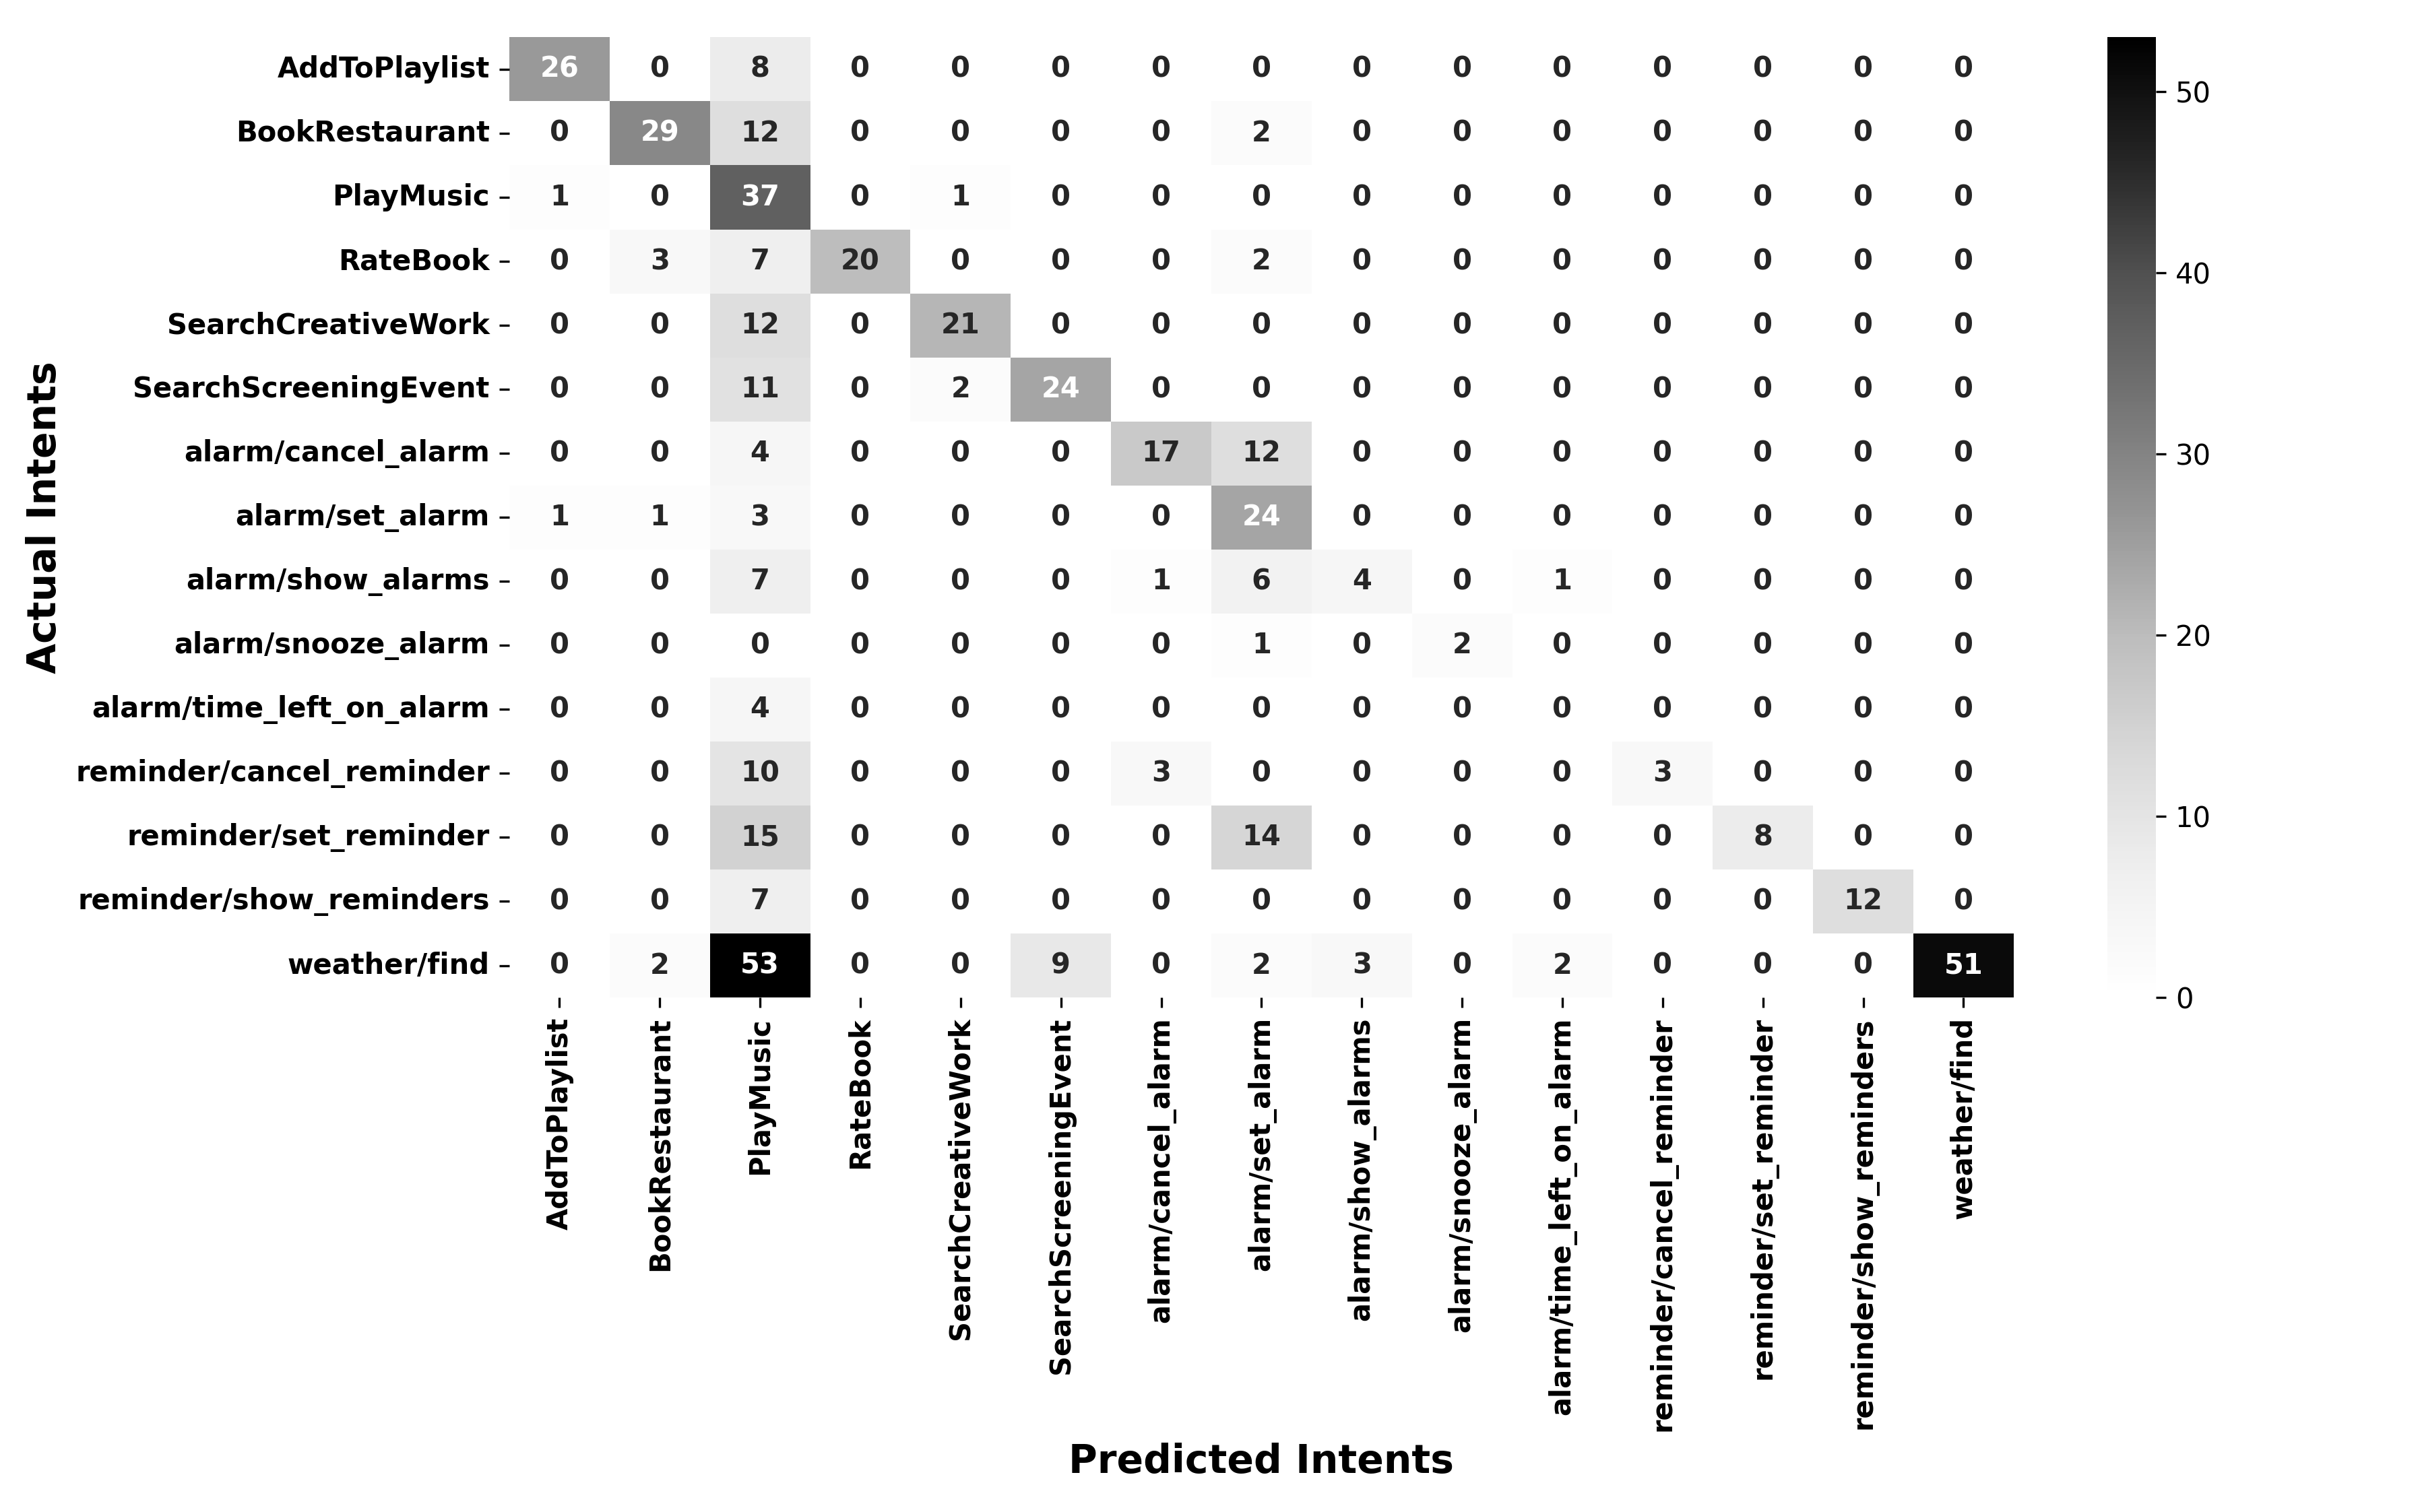
\includegraphics[width=\textwidth]{ma_figures/de-ba_UDxNLU.png}
    \caption{A confusion matrix for the intent classification results of a mDeBERTa model trained on UDxNLU (random-seed=6543) regarding the Bavarian test set created by \citet{winkler-etal-2024-slot-intent} (de-ba).}
    \label{fig:de-ba_UDxNLU}
\end{figure}

\begin{figure}[!ht]
    \centering
    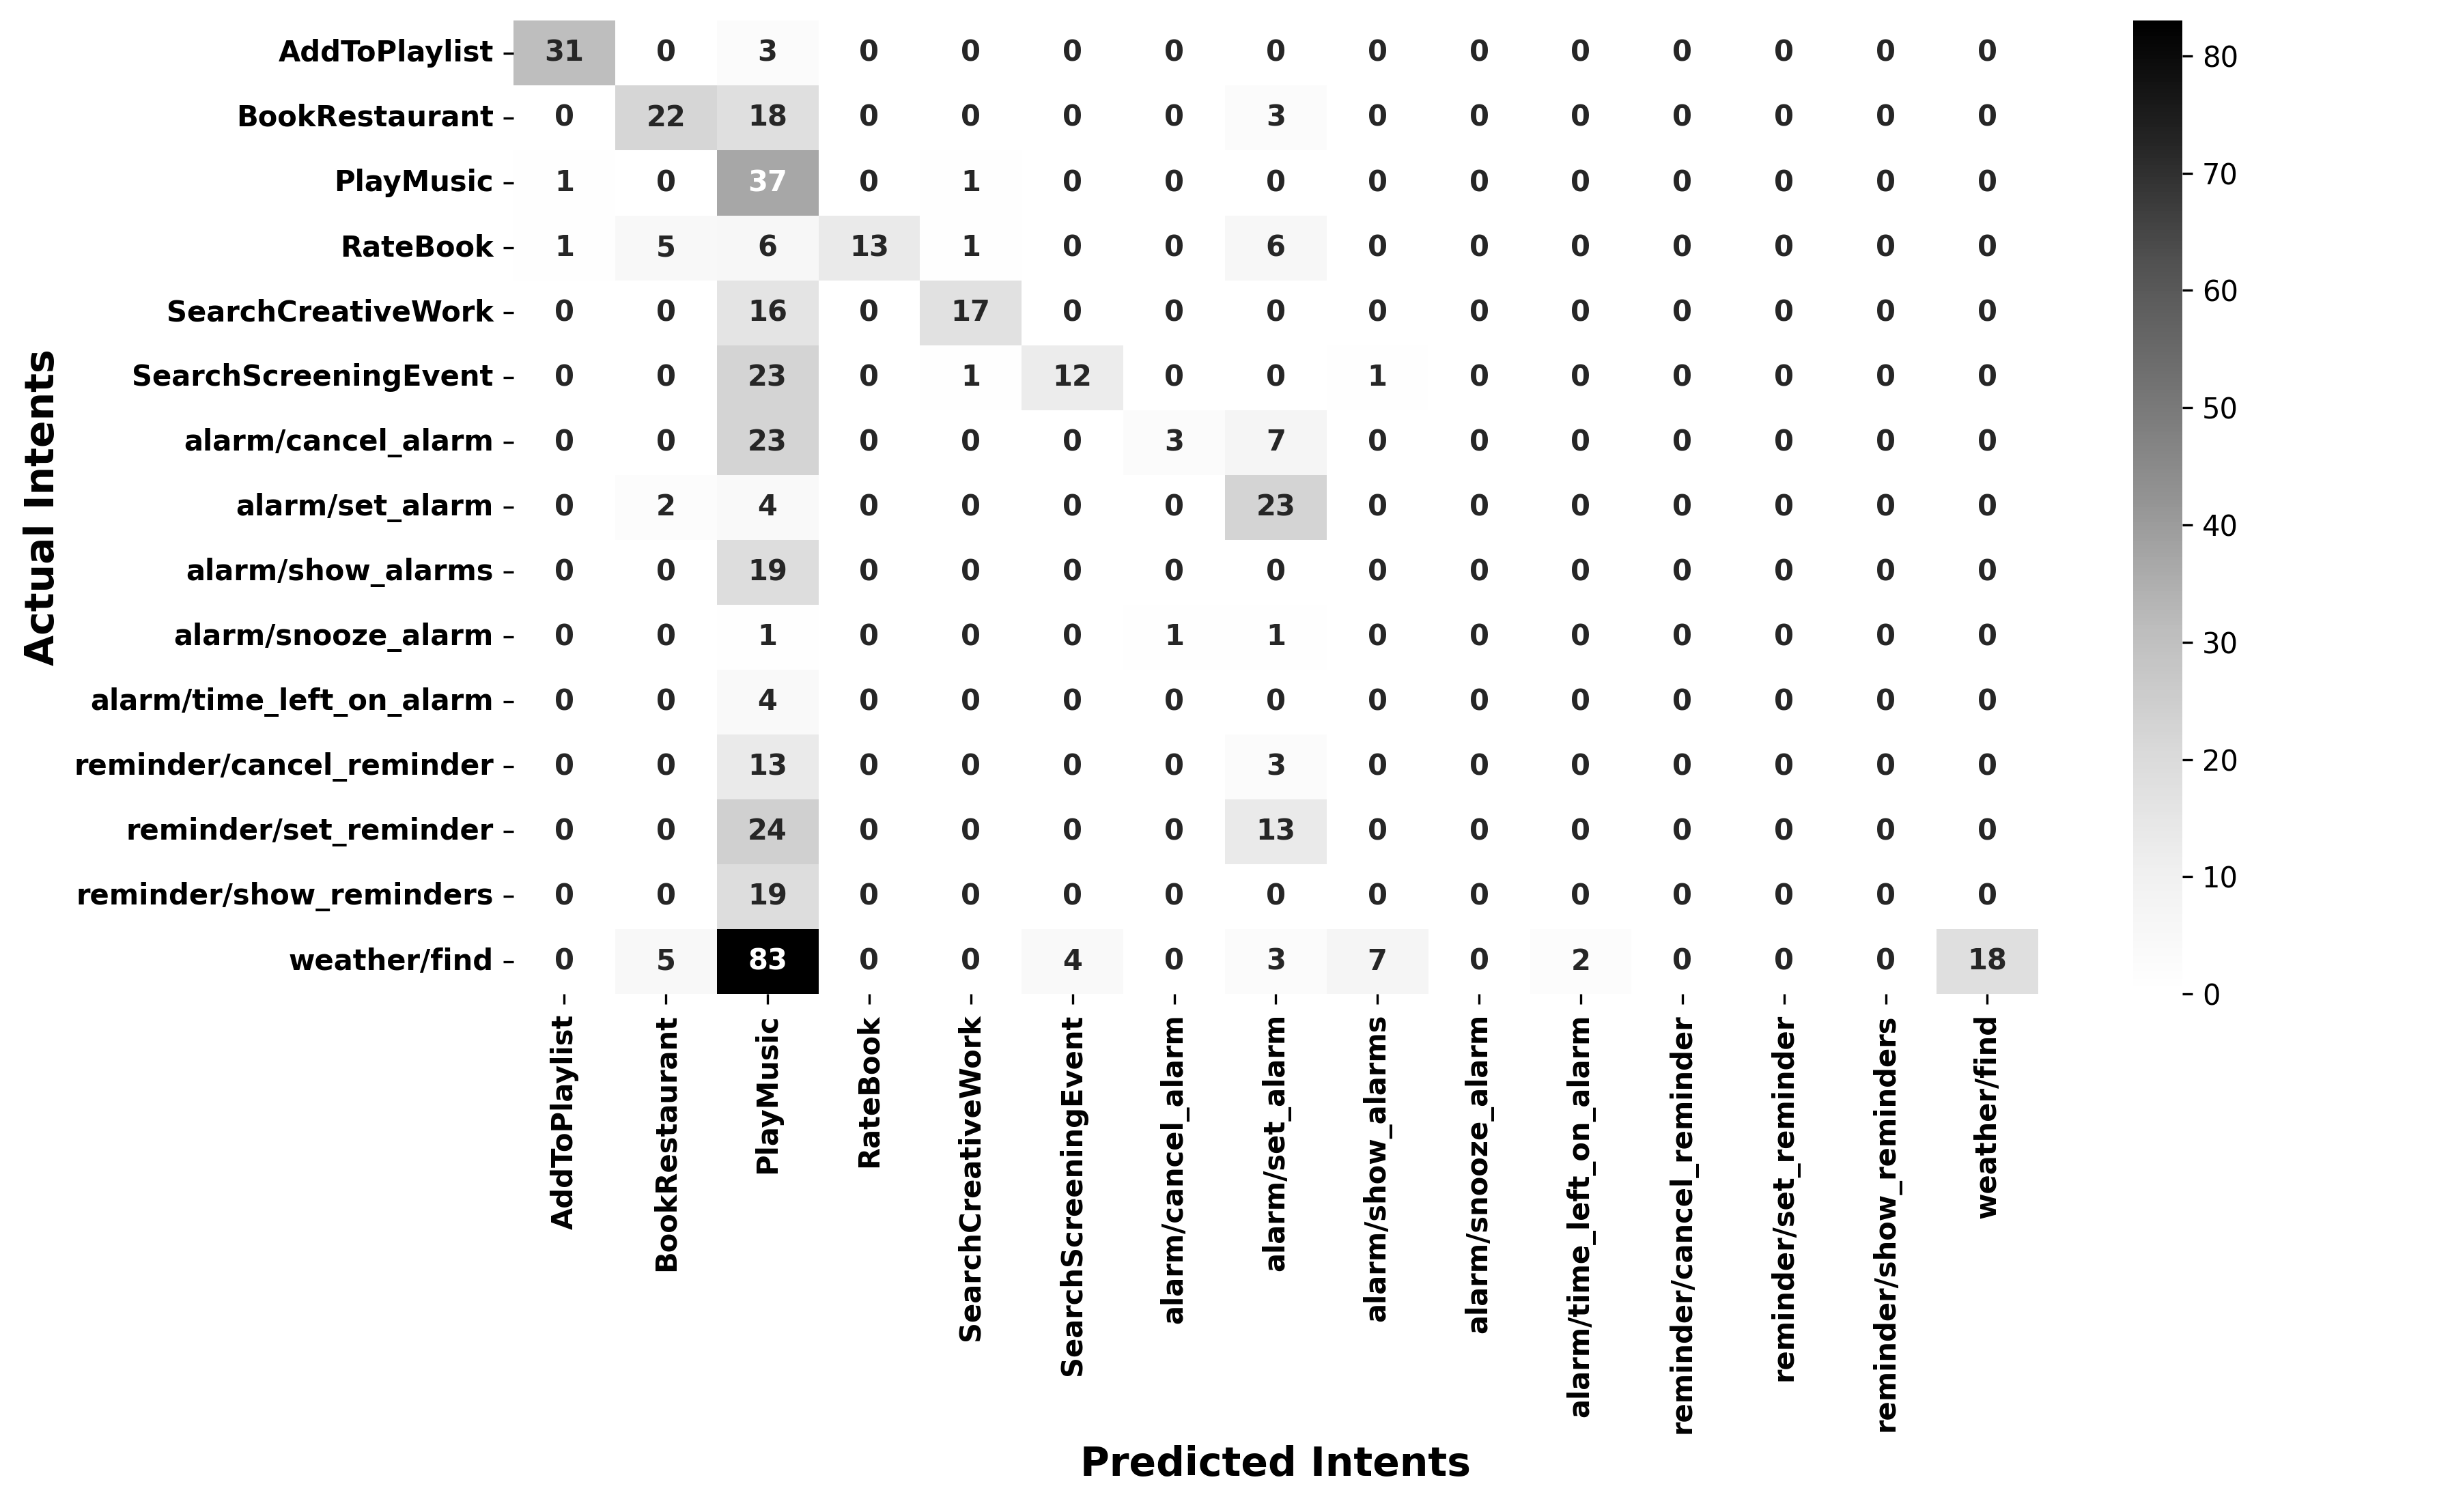
\includegraphics[width=\textwidth]{ma_figures/de-by_UDxNLU.png}
    \caption{A confusion matrix for the intent classification results of a mDeBERTa model trained on UDxNLU (random-seed=6543) regarding the Bavarian test set created in this work (de-by).}
    \label{fig:de-by_UDxNLU}
\end{figure}








\section{Multi-Task Fine-Tuning with Bavarian Named Entity Recognition Data}

This second section on extended experiments shows the results of similarly fine-tuning mDeBERTa in a multi-task setup for zero-shot transfer on slot and intent detection but now with named entity recognition data as an additional task. As outlined in the data chapter, such a corpus is provided for Bavarian named entities by \citet{peng-etal-2024-sebastian-basti} containing two sub-corpora from different sources of Bavarian texts. Based on this, two slightly different tasks for recognising the entities in those sub-corpora could have been made. However, in order to not complicate the fine-tuning process further and to enrich the overall set of entities and examples, NER as only one general task needs to be solved by mDeBERTa in the following. Preliminary attempts have also shown that a the possible diversification of the task rather harms the final SID performance. In order to recreate the two following multi-task settings, access to the second unpublished sub-corpus based on twitter data is necessary. If not available, the experiment can also be run using only the Wikipedia corpus, though. Similarly as for introducing the UD data, NER as an auxiliary task is expected to enhance the performance on slot labelling for Upper German dialects, being a closely related task and introducing this in the target language. From this, the performance on intent classification should also benefit as through the input of this task a lot of general linguistic input in Bavarian is displayed to the model.







\subsection{Basic Sequential Intermediate Setting NER\_NLU}

When adding a new basic configuration file for the NER dataset in which the task type for both sub-datasets is identical as the sequential intermediate setting preceding the NLU configuration, this leads leads to the following results on Upper German dialects averaged over three random seed runs as presented in Table \ref{tab:mDeBERTa_exp2_ner_nlu_dialects}. Training for this setting takes about fifteen minutes longer than for the baseline due to the larger auxiliary dataset. The learning curve on NER reaches a high level after ten epochs already. Slight drops in the following epochs indicate minor generalisation problems. However, as the best results are achieved for the final epochs, training over twenty periods appears suitable. When approaching the average results on the Bavarian and South Tyrolean sets together with their difference to the baseline, an increase in all three metrics can be observed as opposed to the same settings with the UD data. The improvements for slot labelling seem to have made a positive impact on classifying the correct intents as well, though this is probably also rooted in the general contact to Bavarian samples. Similarly, the performance on fully correct examples reaches a new peak for this experiment, carried by the maximum result on the Bavarian test set created in this work. Even more interesting, however, is that this setting led to the highest performance on slot labelling for this Bavarian test set. When thinking back at the dialectal distribution in this corpus which is not well known, Bavarian from the Munich region did not stand out either. However, it appears that the Bavarian Wikipedia or Bavarian tweets are close to this dialectal variety. The low standard deviation on this evaluation set also shows that the models were quite sure on the performance this task. This is not the case concerning the intent classification for the parallel set \textit{de-ba} where more uncertainties seem to prevail. The improved performance on this is thus most likely to be rooted in translations which are closer to the English gold sample structure.

\begin{table}[!ht]
\centering{
\begin{tabular}{l|llllll|ll}
Language      & de   & de-ba & de-by & de-st & en   & gsw  & Avg. & Diff. \\
\hline
slots         & 82.7 & 55.3  & \textbf{53.9}  & 50.2  & 95.4 & 30.1 & 53.1 & 7.8   \\
intents       & 94.2 & 82.8  & 67.7  & 79.1  & 99.2 & 66.2 & 76.6 & 3.1   \\
fully correct & 64.7 & 24.9  & \textbf{21.6}  & 19.6  & 91.0 & 7.9  & 22.0 & 6.9   \\
\hline
sd slots      & 0.6  & 2.3   & 0.5   & 1.4   & 0.3  & 1.4  &  1.3    &  0.2     \\
sd intents    & 0.7  & 3.5   & 0.5   & 1.3   & 0.2  & 3.2  &  1.9   &   -0.3   
\end{tabular}}
\caption{Results for the basic sequential intermediate NER\_NLU experiment with mDeBERTa according to Upper German dialects over three random seeds, Avg. = average on languages without English, German and Swiss German, Diff. = average performance difference to mDeBERTa baseline, sd = standard deviation}
\label{tab:mDeBERTa_exp2_ner_nlu_dialects}
\end{table}





\subsection{Basic Multi-Task Setting NERxNLU}

Training mDeBERTa on a multi-task configuration file containing these NER sets but only one task type together with both SID task types leads to quite similar results as within the sequential experiment before, showcased in Table \ref{tab:mDeBERTa_exp2_nernlu_dialects}. Fine-tuning mDeBERTa on this setting takes one hour and twenty minutes. When analysing the learning curves, which are not as smooth and linear for slot labelling and entity recognition in this configuration, finishing a bit earlier than 20 epochs can be considered too much. In most cases, the maximum level of performance on the development set is already reached by then. In more detail on the results, the overall performance on slot labelling increases slightly whilst the number for intent detection decreases a bit, similarly to the amount of fully correct examples. In order to pre-rank the result of + 8.5 on strict slot F1 score, this is the third highest average across the three Upper German dialects. This effort could be even higher when the performance on Swiss German was part of the average calculation, reaching it's highest result across all other extended multi-task experiments in this setting. Apart from this, the most interesting part of these results is the very low standard deviations for both slots and intents. This shows that these numbers are quite solid against random seed variation, proving the robustness of the multi-task fine-tuned models and their ability to generalise on SID via zero-shot transfer upon low-resource dialects. As opposed to the UD data which leads to confusion in such a multi-task scenario, NER as a closely related auxiliary task to SID further enhances the model's capabilities on this overall target task.

\begin{table}[!ht]
\centering{
\begin{tabular}{l|llllll|ll}
Language      & de   & de-ba & de-by & de-st & en   & gsw  & Avg. & Diff. \\
\hline
slots         & 82.2 & 55.9  & 52.5  & 52.9  & 95.0 & \textbf{33.3} & 53.8 & 8.5   \\
intents       & 94.9 & 82.8  & 66.3  & 79.6  & 99.1 & 65.1 & 76.2 & 2.7   \\
fully correct & 63.5 & 25.6  & 18.5  & 19.6  & 90.3 & 10.1 & 21.2 & 6.1   \\
\hline
sd slots      & 1.1  & 1.1   & 1.8   & 0.9   & 0.2  & 0.1  &  1.0    &  0.5     \\
sd intents    & 1.2  & 1.8   & 1.6   & 1.0   & 0.1  & 1.1  &  1.4    &  0.2    
\end{tabular}}
\caption{Results for the basic multi-task NERxNLU experiment with mDeBERTa according to Upper German dialects over three random seeds, Avg. = average on languages without English, German and Swiss German, Diff. = average performance difference to mDeBERTa baseline, sd = standard deviation}
\label{tab:mDeBERTa_exp2_nernlu_dialects}
\end{table}








\section{(Multi-Task) Continuous Pre-Training with Bavarian Masked-Language-Modeling Data}

A slightly different title needs to be chosen when describing this third section of extended experiments showing the results of fine-tuning mDeBERTa in a multi-task setup with an auxiliary task for zero-shot transfer on slot and intent detection. Using masked language modelling as such an additional task, it is suitable to be talked about continuous pre-training for this approach. As described within the respective section below the data chapter, pre-processed Bavarian data, i.e. medium to large sized sentences, is taken from \citet{artemova-plank-2023-low} where it was created for bilingual lexicon induction and thus of high quality. Since pre-training is generally used to introduce models to linguistic peculiarities of a certain target language or domain, it can be expected that by doing so, both slot and intent detection as successive or side-tasks profit from Bavarian input when being transferred in a zero-shot manner to Upper German dialects in the following. However, \citet{dery2022pretraining} show in their paper on the question whether pre-training should actually be done that on low-resource NLP tasks, a better performance can be reached through multi-task training with similar auxiliary tasks instead of continuous pre-training.






\subsection{Basic Sequential Intermediate Continuous Pre-Training Setting MLM\_ NLU}

Starting with the case of performing continuous pre-training with a language or domain specific corpus to then fine-tune the further pre-trained model in a sequential manner upon the target task, the results of this process for mDeBERTa and the given Upper German evaluation datasets are displayed in Table \ref{tab:mDeBERTa_exp3_mlm_nlu_dialects}. Although the process requires large resources of graphical processing units, continuous pre-training on the 1.250 sentences takes less than five minutes for twenty epochs. When looking at the learning curve, the perplexity drops sharply after around five epochs already. This suggests that only a few epochs are enough. Going through twenty is not further time and resource consuming, though. In each of the five random seed runs, the model then fine-tuned on SID reached it's best result after the twentieth epoch. This suggests that training on more epochs is actually more rewarding after continuous pre-training - a finding that could be a solution to improve the low results obtained in this setting. In all metrics, the baseline is undercut, especially for slot detection. As the results for English and German are still stable, the decline can clearly be drawn upon Upper German dialects. It seems that the multilingual model is rather distracted from it's existing representations through continuous pre-training with Bavarian data regarding this and closely related varieties. In a second step, it is then not capable of capturing the inputs for solving SID anymore. A possible solution could be increasing the number of epochs in order to provide the model with more opportunities to modify it's representations for SID after them being adapted through continuous pre-training. 

\begin{table}[!ht]
\centering{
\begin{tabular}{l|llllll|ll}
Language      & de   & de-ba & de-by & de-st & en   & gsw  & Avg. & Diff. \\
\hline
slots         & 78.7 & 40.8  & 37.4  & 40.5  & 94.8 & 18.1 & 39.6 & -5.7  \\
intents       & 94.4 & 77.8  & 62.5  & 75.0  & 99.3 & 58.9 & 71.8 & -1.7  \\
fully correct & 58.3 & 14.9  & 9.0   & 12.3  & 90.1 & 3.9  & 12.1 & -3.0  \\
\hline
sd slots      & 1.6  & 4.1   & 2.9   & 3.4   & 0.6  & 2.0  &  2.9    &  -1.4     \\
sd intents    & 2.4  & 2.9   & 2.2   & 1.8   & 0.2  & 5.2  &  2.9    &  -1.3   
\end{tabular}}
\caption{Results the for the basic sequential intermediate MLM\_NLU experiment with mDeBERTa according to Upper German dialects over three random seeds, Avg. = average on languages without English, German and Swiss German, Diff. = average performance difference to mDeBERTa baseline, sd = standard deviation}
\label{tab:mDeBERTa_exp3_mlm_nlu_dialects}
\end{table}







\subsection{Basic Mulit-Task Continuous Pre-Training Setting MLMxNLU}

In order to root back the confusions created by continuously pre-training mDeBERTa on a small amount of Bavarian text to the sequential manner of the previous experiment, a further attempt is made using a multi-task configuration that consist of masked language modeling as a task together with the NLU configuration for SID. Similarly in this setting, adding continuous pre-training only increases the time for training and evaluation of a model by five minutes over the baseline duration. Here, the graphical storage requirement is a also a lot higher, though. In each run on three different random seeds, the model extracted after the twentieth training epoch gives the best results. Again, training on more epochs could lead to better results, enabling the model to further adapt it's representations. As can be seen in Table \ref{tab:mDeBERTa_exp3_mlmnlu_dialects}, these get only slightly better as before, especially for slot detection, though still presenting a downgrade on average as opposed to the baseline. A possible reason could be once more that masked language modelling confuses the model when trying to adapt its representations for SID instead of enabling it to understand the structure and orthography of Bavarian to be able to transfer to Upper German dialects in general. Another reason could be that the model is not able to connect both tasks, i.e. to moderate between capturing the new language and similarly solving SID. Finally, another hypothesis could be that knowledge of SID is slightly lost whilst generally knowing Bavarian increases which can not be seen in the performance on SID, though. The actual reason, possibly rooted in these assumptions somewhere, is hard to detect. What can be said, however, is that performing continuous pre-training does make mDeBERTa change it's representations. It is this experiment for which the best slot detection and fully correct results were reached in English. Thus, it can be expected that the reorganisation of some parameters via masked language modelling also may help for a distant and similarly trained target task after all. Whilst approaching this via larger amounts of text or training for more epochs is not pursued due to low-resource computational power, MLM is still incorporated in extended multi-task experiments for zero-shot transfer learning on SID in the following.

\begin{table}[!ht]
\centering{
\begin{tabular}{l|llllll|ll}
Language      & de   & de-ba & de-by & de-st & en   & gsw  & Avg. & Diff. \\
\hline
slots         & 82.2 & 45.5  & 42.0  & 46.3  & \textbf{96.1} & 21.2 & 44.6 & -0.7  \\
intents       & 95.3 & 76.9  & 61.5  & 77.3  & 99.2 & 56.8 & 71.9 & -1.6  \\
fully correct & 63.2 & 16.4  & 11.9  & 14.6  & \textbf{91.9} & 3.8  & 14.3 & -0.8  \\
\hline
sd slots      & 0.7  & 2.0   & 1.4   & 1.6   & 0.2  & 1.8  &  1.5    &  0.0     \\
sd intents    & 1.3  & 2.1   & 2.1   & 0.5   & 0.2  & 3.4  &  1.9    &  -0.3    
\end{tabular}}
\caption{Results for the basic continuous pre-training MLMxNLU experiment with mDeBERTa according to Upper German dialects over three random seeds, Avg. = average on languages without English, German and Swiss German, Diff. = average performance difference to mDeBERTa baseline, sd = standard deviation}
\label{tab:mDeBERTa_exp3_mlmnlu_dialects}
\end{table}







\section{Accumulated Multi-Task Fine-Tuning with Bavarian Data}

This fourth round of experiments now makes use of combinations amongst multiple of the previous tasks and procedures. In other words, several multi-task configurations of such experiments are compiled for this purpose whilst also the single-task configurations used as above will be used for sequential experiments with multiple steps. The main motivation for these accumulated experiments is that all of the previous three auxiliary tasks have contributed to improved results at least in some way. The question that arises from this is whether certain or an overall combination leads to even better results on zero-shot cross-lingual transfer to SID in Upper German dialects. Referring to extended experiments in the following builds only on adding new, extended configuration files or using the existing in further steps. It does not stand for an expansion of the training data or a change in other parameters. At first, two multi sequential and three extended multi-task settings will be tried out. Finally, both of these settings are combined in three additional experiments, resulting in the best overall approach. A closer analysis on the key findings will then be made in the next chapter, addressing the second research question of this thesis.





\subsection{Extended Multi-Sequential Intermediate Setting UD\_NER\_NLU}

In a first extended experiment, it is analysed whether multi-step sequential intermediate tasks training improve the zero-shot transfer performance on SID, the ultimate target task in the sequence, for Upper German dialects. The main insight of the basic experiments of this kind of procedure is that using both UD and NER as intermediate auxiliary task data leads to an improved performance. Since this is larger and more stable for NER, this is set as the task in the middle, further refining the representational changes that are being made through fine-tuning on UD data at the beginning of this experiment. The results of this progression for which no new configuration files need to be created can be seen in Table \ref{tab:mDeBERTa_exp4_ud_ner_nlu_dialects}, averaged again over three random seed runs. Training mDeBERTa on these tasks takes two hours, much longer than for previous attempts. Interestingly, apart from two runs in which the best model on SID resulted from the last epoch, number twenty, one run reaches it's maximum performance on the development set in epoch fifteen already. A detailed analysis shows that this is very close, though, as epoch twenty is close to the top result as well. The learning curves of all tasks follow similar patterns as before. Thus, it is not surprising that this experiment leads to one of the best overall average performances. Especially for slot detection in Bavarian and South Tyrolean, but also for Swiss German, a top-notch result for cross-lingual transfer learning is reached. It has to be mentioned, though, that the standard deviation for slots is slightly higher than in the baseline. Concerning intent detection, a similarly good performance is achieved which is also reflected in the amount of fully correct annotated examples. Fine-tuning sequentially on multiple auxiliary tasks in the target language and finally on the target task thus creates representations in the embeddings which are beneficial for zero-shot cross-lingual transfer on this last task.

\begin{table}[!ht]
\centering{
\begin{tabular}{l|llllll|ll}
Language      & de   & de-ba & de-by & de-st & en   & gsw  & Avg. & Diff. \\
\hline
slots         & 82.3 & 56.4  & 53.6  & 53.0  & 95.4 & 30.7 & 54.3 & 9.0   \\
intents       & 96.3 & 84.3  & 69.9  & 80.7  & 99.1 & 65.4 & 78.3 & 4.8   \\
fully correct & 65.1 & 24.9  & 21.5  & 21.5  & 90.7 & 7.4  & 22.6 & 7.5   \\
\hline
sd slots      & 1.9  & 3.6   & 1.9   & 3.2   & 0.5  & 2.4  &  2.7   &  -1.2     \\
sd intents    & 0.7  & 2.9   & 1.0   & 1.5   & 0.1  & 1.8  &  1.6   &    0.0  
\end{tabular}}
\caption{Results the for extended multi-sequential intermediate UD\_NER\_NLU experiment with mDeBERTa according to Upper German dialects over three random seeds, Avg. = average on languages without English, German and Swiss German, Diff. = average performance difference to mDeBERTa baseline, sd = standard deviation}
\label{tab:mDeBERTa_exp4_ud_ner_nlu_dialects}
\end{table}






\subsection{Extended Multi-Sequential Intermediate Setting MLM\_NER\_NLU}

This present experiment is mainly conducted in order to test whether the negative impact of continuous pre-training on the basic sequential experiment also holds true in a multi-sequential intermediate task setting with MLM as the initial and NER as the middle task. Each run in this setting takes two hours and ten minutes with no differences to previously described learning curves. The best model according to the English SID development set is reached in the nineteenth and one time on the twentieth epoch. Thus, this number of training sessions appears to be suitable. When analysing the results provided in Table \ref{tab:mDeBERTa_exp4_mlm_ner_nlu_dialects}, it becomes apparent that on average an improvement over the baseline is reached, not over the previous experiment, though. Apart from this and especially due to the more costly training time and resources, it is decided to not implement any further experiments in other combinations, successions or in an overall multi-sequential intermediate MLM\_UD\_NER\_NLU setting. In this context, now, MLM does not harm the performance on Upper German dialects. In fact, regarding the intent detection in German, it actually leas to a new maximum performance on this language which is close to Upper German dialects. Similarly striking is the low average standard deviation for both tasks, showcasing that the experiment produces quite robust models for transfer learning on SID.

\begin{table}[!ht]
\centering{
\begin{tabular}{l|llllll|ll}
Language      & de   & de-ba & de-by & de-st & en   & gsw  & Avg. & Diff. \\
\hline
slots         & 80.0 & 53.4  & 51.8  & 49.3  & 95.1 & 29.5 & 51.5 & 6.2   \\
intents       & \textbf{97.3} & 83.3  & 66.7  & 80.5  & 99.2 & 64.3 & 76.8 & 3.3   \\
fully correct & 63.4 & 23.5  & 19.1  & 20.7  & 90.3 & 7.0  & 21.1 & 6.0   \\
\hline
sd slots      & 0.3  & 0.9   & 1.7   & 1.4   & 0.3  & 0.9  &  1.1    &  0.4     \\
sd intents    & 0.5  & 1.6   & 1.0   & 1.1   & 0.2  & 1.9  &  1.3    &  0.3    
\end{tabular}}
\caption{Results the for extended multi-sequential intermediate MLM\_NER\_NLU experiment with mDeBERTa according to Upper German dialects over three random seeds, Avg. = average on languages without English, German and Swiss German, Diff. = average performance difference to mDeBERTa baseline, sd = standard deviation}
\label{tab:mDeBERTa_exp4_mlm_ner_nlu_dialects}
\end{table}




\subsection{Extended Multi-Task Setting UDxNERxNLU}

Instead of performing further sequential experiments which are also quite unhandy regarding storage requirements, extended multi-task experiments are conducted from now on for this and the two following paragraphs. Concretely, this means using two or all three possible additional tasks together in one configuration file with SID. In a first step, equivalently to the sequential approach, UD and NER are chosen as datasets for these tasks. Fine-tuning on them takes only one hour and twenty minutes, much less than for the sequential approach. All top models on the development sets are reached in the final two epochs whose number can thus be enlarged for a possibly even better performance. Whats interesting in the learning curves is now that the performance on the auxiliary tasks only starts to be trained from the second to fifth epoch. Until this, major progress is initially made for SID, which is also rooted in the much larger training set. In contrast to this, however, this attempt leads to contrary results as being displayed in Table \ref{tab:mDeBERTa_exp4_udnernlu_dialects}. Whilst the performance decline on slot labelling is marginally on the average for the core Upper German dialects and the fully correct examples are on a par to the baseline, the decline regarding intent classification accuracy by almost eleven percent is tough, also because the average standard deviation for this task is not unusually large. As can be seen from the strong results on the English evaluation set, this trend is particular to Upper German dialects. Apart from Swiss German, the numbers of the Upper Bavarian evaluation set \textit{de-ba} has suffered a higher performance loss as compared to the test set from this thesis, \textit{de-by}. When aiming to find possible reasons for this picture, a first one is increased confusion being brought in to this fine-tuning process in which five sub-tasks need to be solved by the model simultaneously. In such a larger multi-task setting, introducing distinct tasks like those in the UD set might confuse the rearrangement of representations for the actual target task. Since this is trained via the much larger dataset, however, it rather appears to be a change in the cross-lingual capabilities introduced by the Bavarian auxiliary task data causing the confusion. When considering the learning curves, a final reason could be unfinished training on the auxiliary tasks by the stopping criterion of only twenty epochs.

\begin{table}[!ht]
\centering{
\begin{tabular}{l|llllll|ll}
Language      & de   & de-ba & de-by & de-st & en   & gsw  & Avg. & Diff. \\
\hline
slots         & 78.4 & 45.9  & 44.1  & 44.1  & 95.3 & 25.7 & 44.7 & -0.6  \\
intents       & 93.0 & 65.4  & 54.8  & 67.7  & 99.3 & 46.4 & 62.6 & -10.9 \\
fully correct & 57.4 & 16.7  & 14.0  & 14.7  & 90.7 & 5.9  & 15.1 & 0.0   \\
\hline
sd slots      & 2.4  & 5.1   & 2.6   & 5.3   & 0.4  & 5.0  &  4.2    &  -2.7     \\
sd intents    & 0.9  & 3.5   & 2.4   & 1.1   & 0.1  & 3.1  &  2.2    &  -0.4    
\end{tabular}}
\caption{Results for the extended multi-task UDxNERxNLU experiment with mDeBERTa according to Upper German dialects over three random seeds, Avg. = average on languages without English, German and Swiss German, Diff. = average performance difference to mDeBERTa baseline, sd = standard deviation}
\label{tab:mDeBERTa_exp4_udnernlu_dialects}
\end{table}





\subsection{Extended Multi-Task Setting MLMxNERxNLU}

Although introducing MLM as an additional auxiliary task reduced the performance of zero-shot cross-lingual transfer on SID in the basic multi-task setting and did not enhance it in the sequential approach either, it is tried out in a multi-task configuration combination with NER to attend NLU here again. As can be seen in the averaged results in Table \ref{tab:mDeBERTa_exp4_mlmnernlu_dialects}, the exhausting training time of a little over two hours which should actually be extended as the best model was reached on the development data in the last of the twenty epochs is worth the effort. Regarding slot detection, the average over three random seed runs on this settings reveals a maximum performance for German, Upper Bavarian and South Tyrolean, resulting in the top slot detection average for the three core Upper German dialects. This is rounded of by a low average standard deviation for this task. When turning towards intent classification, this average performance improved to some extent as well. Interestingly, however, this configuration leads to the highest number reached throughout all experiments for intent detection on the English evaluation set. Finally, this experiment achieves the highest amount of fully correct annotated examples in Swiss German. This being a little over ten percent accuracy, however, cannot be seen as a major success. When trying to classify these results, it seems that masked language modeling with Bavarian data in connection with NER, a similar task to SID and similarly in the target language enhances the capabilities of the model in both understanding linguistic specialities of Upper German varieties and, in particular, the task of slot labelling. In a multi-task setting, this works even better as fine-tuning on these tasks sequentially. A similar improve for intent classification leads to the same trend on the amount of fully correct annotated examples.

\begin{table}[!ht]
\centering{
\begin{tabular}{l|llllll|ll}
Language      & de   & de-ba & de-by & de-st & en   & gsw  & Avg. & Diff. \\
\hline
slots         & \textbf{83.0} & \textbf{56.6}  & 53.7  & \textbf{54.2}  & 95.5 & 32.7 & \textbf{54.8} & 9.5   \\
intents       & 95.3 & 84.7  & 67.7  & 81.2  & \textbf{99.4} & 69.1 & 77.9 & 4.4   \\
fully correct & 64.9 & 25.6  & 20.1  & 21.3  & 91.2 & \textbf{10.3} & 22.3 & 7.2   \\
\hline
sd slots      & 0.9  & 0.3   & 1.1   & 1.5   & 0.3  & 0.9  &  1.2    &   0.3    \\
sd intents    & 1.0  & 0.5   & 1.0   & 2.6   & 0.2  & 3.3  &  1.7    &   -0.1   
\end{tabular}}
\caption{Results for the extended multi-task MLMxNERxNLU experiment with mDeBERTa according to Upper German dialects over three random seeds, Avg. = average on languages without English, German and Swiss German, Diff. = average performance difference to mDeBERTa baseline, sd = standard deviation}
\label{tab:mDeBERTa_exp4_mlmnernlu_dialects}
\end{table}





\subsection{Extended Multi-Task Setting MLMxUDxNERxNLU}

Based upon the advances within the previous experiment, a last configuration was created including all auxiliary tasks to stand by SID. Training upon this most extensive setting similarly takes around two hours and twenty minutes. Again, further training on more than twenty epochs could lead to improved results as for all three runs on random seeds, the performance on the development sets is at highest in the last epoch. Considering the results displayed in Table \ref{tab:mDeBERTa_exp4_mlmudnernlu_dialects}, however, investing more time in further fine-tuning is not promising. Whilst a small increase on slot detection can be found on the average, the second largest downgrade of minus fifteen percent in accuracy can be observed for intent classification on the three Upper German dialects. Additionally, the standard deviation for this task is relatively high. A slight improvement for the amount of fully correct annotations also shows the detachment of this metric from intent detection. When searching for reasons for this performance, similarities to the smaller multi-task setting UDxNERxNLU appear where introducing UD data seems to harm the model regarding intent classification as well. Of course, the amount of different tasks that are to be considered by the base mDeBERTa model might be to high to establish respective task and language specific representations in the final embedings.

Due to the poor result, a closer look into confusion matrices for intent detection is made here as well. The first plot in Figure \ref{fig:de-ba_MLMxUDxNERxNLU} for \textit{de-ba} shows that in this experiment, the fine-tuned mDeBERTa model has issues to differentiate the intent \textit{AddToPlaylist}. This is mistaken almost for every other of the fifteen intents in the test set, most frequently by the unrelated intent \textit{weather/find} but also by \textit{reminder/set\_reminder} and intents regarding the domain of setting, showing or cancelling an alarm. Apart from this, no other miss-classifications exist. A similar picture emerges in Figure \ref{fig:de-by_MLMxUDxNERxNLU} for \textit{de-by} where \textit{AddToPlaylist} is even more frequently mistaken for \textit{weather/find}, though. In return, other erroneous classifications are made, most of them for \textit{alarm/set\_alarm} which is again mistaken for cancelling alarms or setting reminders. Overall, however, this leads to the lower accuracy as displayed in Table \ref{tab:mDeBERTa_exp4_mlmudnernlu_dialects}. Using a specific F1 score for intent classification would enable a closer analysis on this matter.

\begin{table}[!ht]
\centering{
\begin{tabular}{l|llllll|ll}
Language      & de   & de-ba & de-by & de-st & en   & gsw  & Avg. & Diff. \\
\hline
slots         & 81.0 & 50.4  & 46.3  & 49.3  & 95.6 & 28.7 & 48.7 & 3.4   \\
intents       & 89.8 & 62.1  & 49.1  & 62.7  & 99.1 & 42.0 & 58.0 & -15.5 \\
fully correct & 58.9 & 19.1  & 15.1  & 16.7  & 91.1 & 7.4  & 17.0 & 1.9   \\
\hline
sd slots      & 0.7  & 2.3   & 1.2   & 1.1   & 0.4  & 0.8  &  1.3    &  0.2     \\
sd intents    & 0.9  & 4.6   & 5.8   & 3.6   & 0.2  & 8.3  &   4.7   &  -3.1   
\end{tabular}}
\caption{Results for the extended multi-task MLMxUDxNERxNLU experiment with mDeBERTa according to Upper German dialects over three random seeds, Avg. = average on languages without English, German and Swiss German, Diff. = average performance difference to mDeBERTa baseline, sd = standard deviation}
\label{tab:mDeBERTa_exp4_mlmudnernlu_dialects}
\end{table}

% figures to show possible issues for intent detection in the Bavarian evaluatio sets
\begin{figure}[!ht]
    \centering
    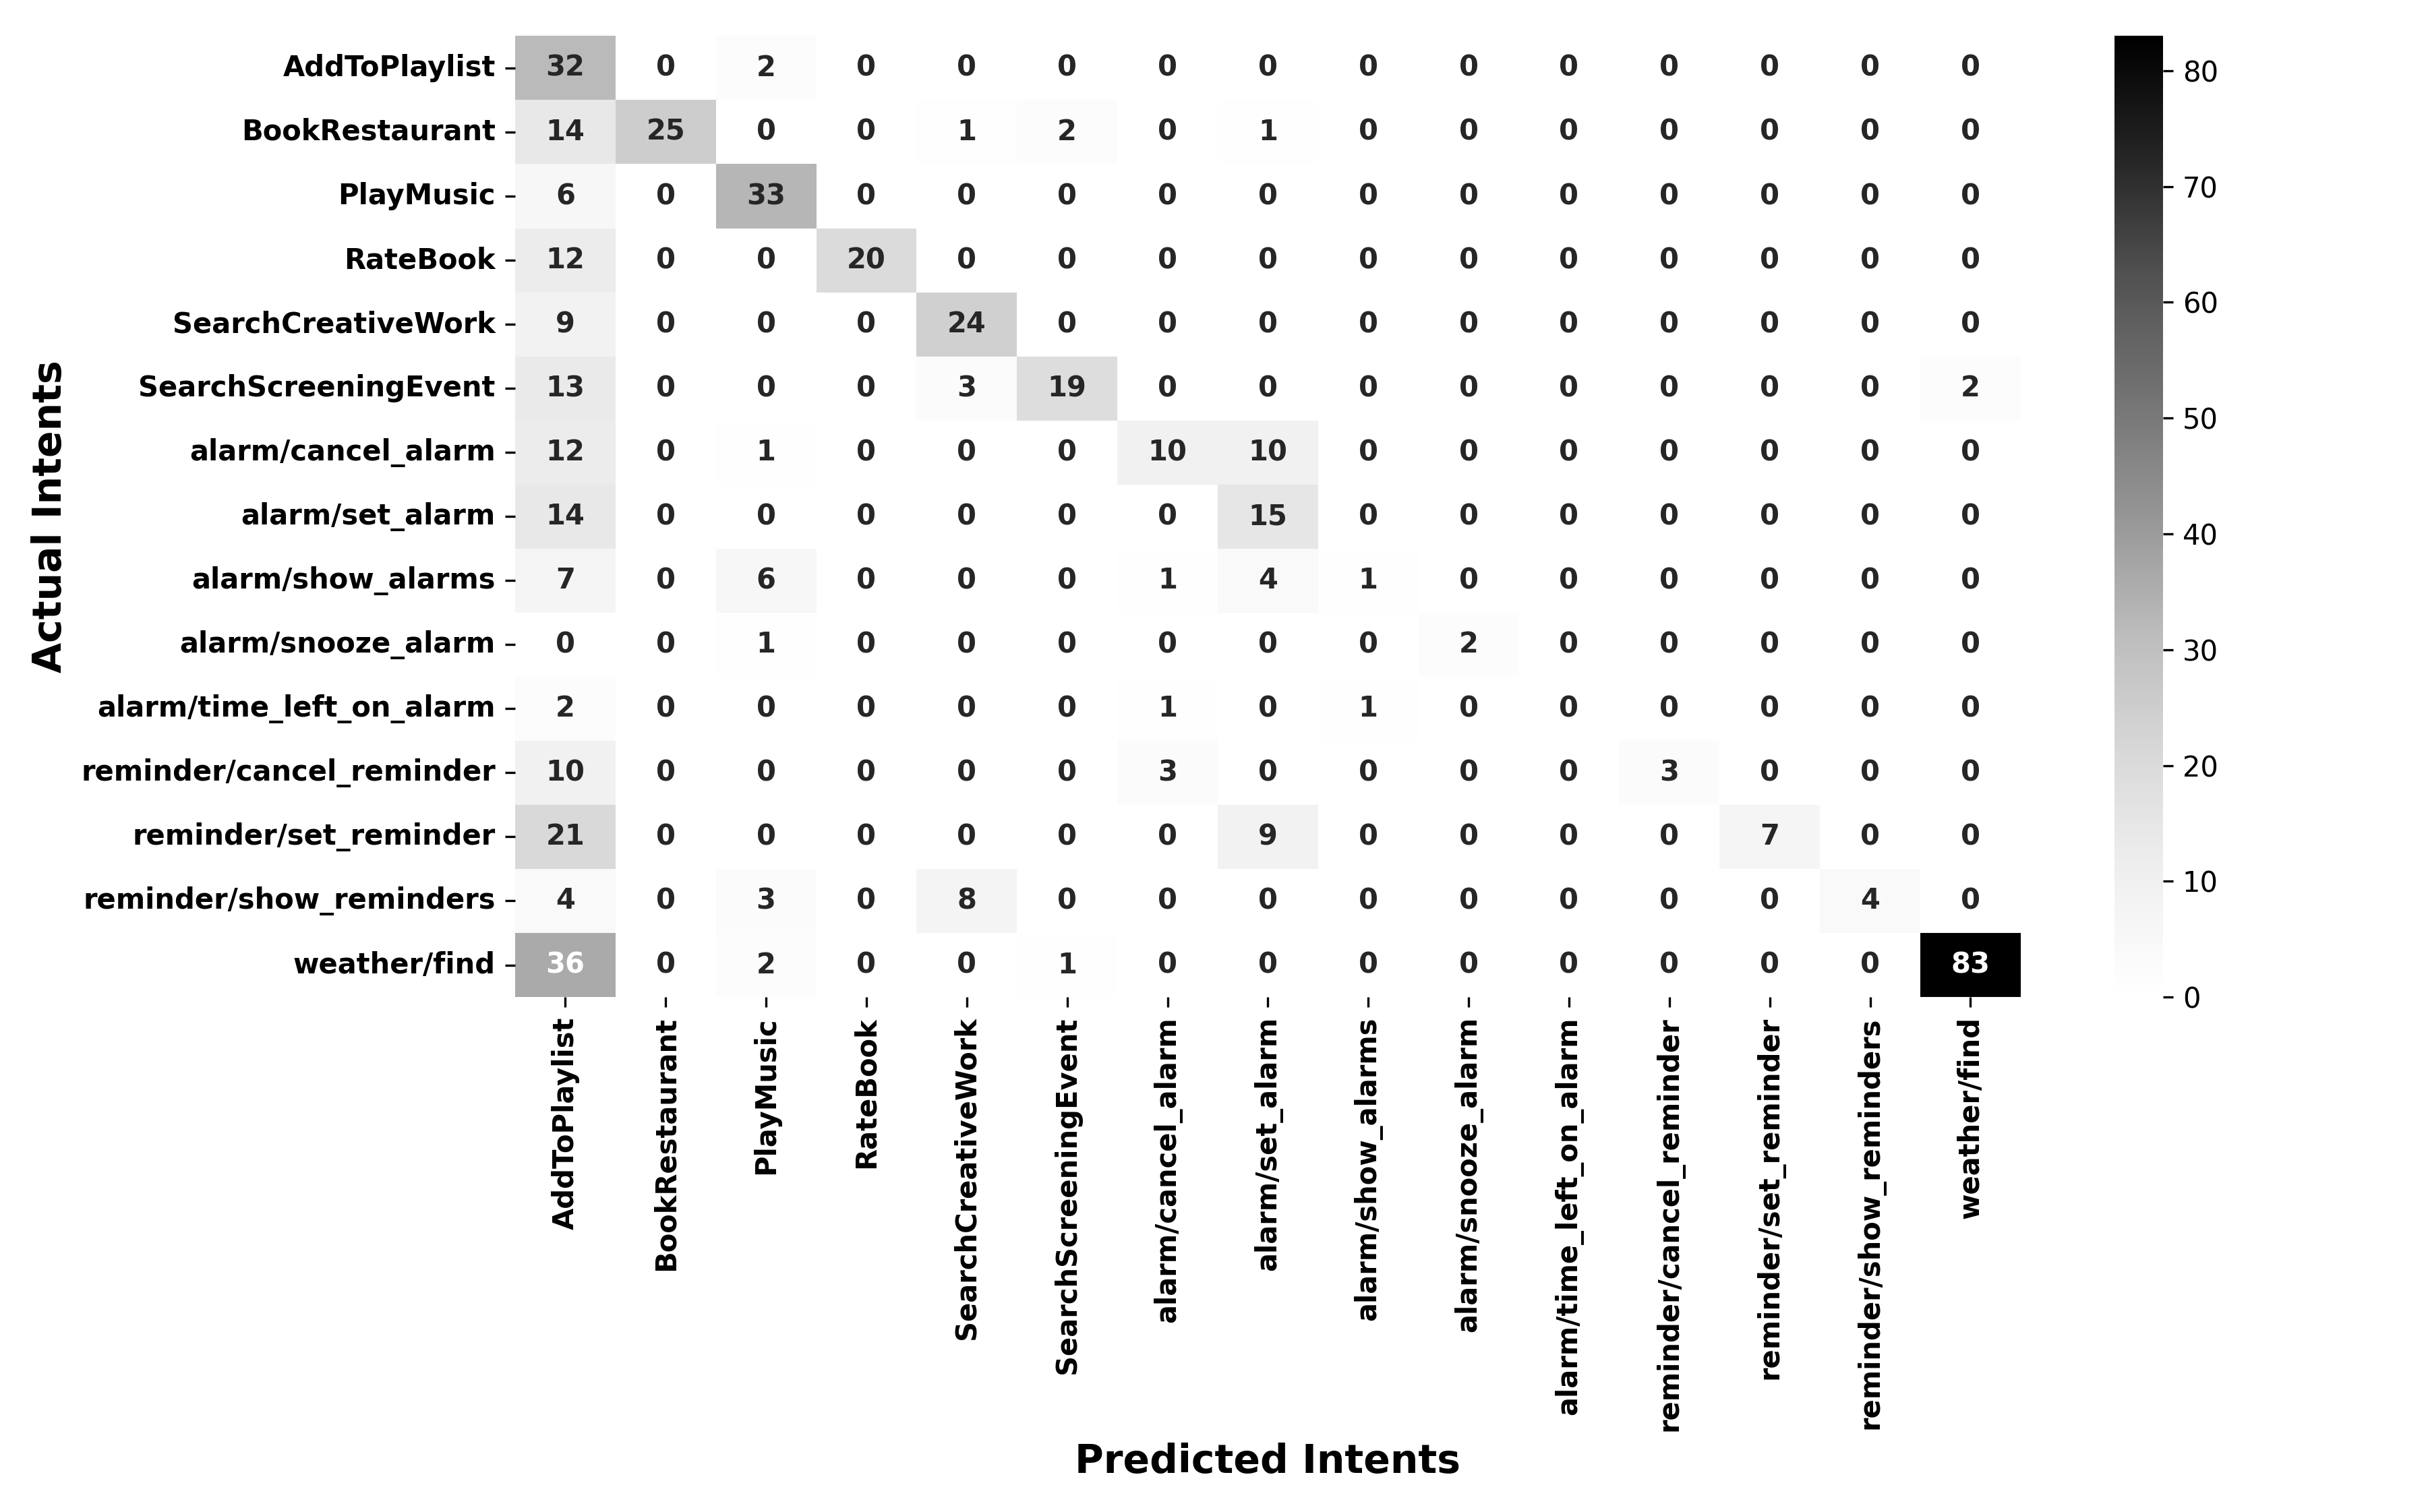
\includegraphics[width=\textwidth]{ma_figures/de-ba_MLMxUDxNERxNLU.png}
    \caption{A confusion matrix for the intent classification results of a mDeBERTa model trained on MLMxUDxNERxNLU (random-seed=6543) regarding the Bavarian test set created in this work (de-ba).}
    \label{fig:de-ba_MLMxUDxNERxNLU}
\end{figure}

\begin{figure}[!ht]
    \centering
    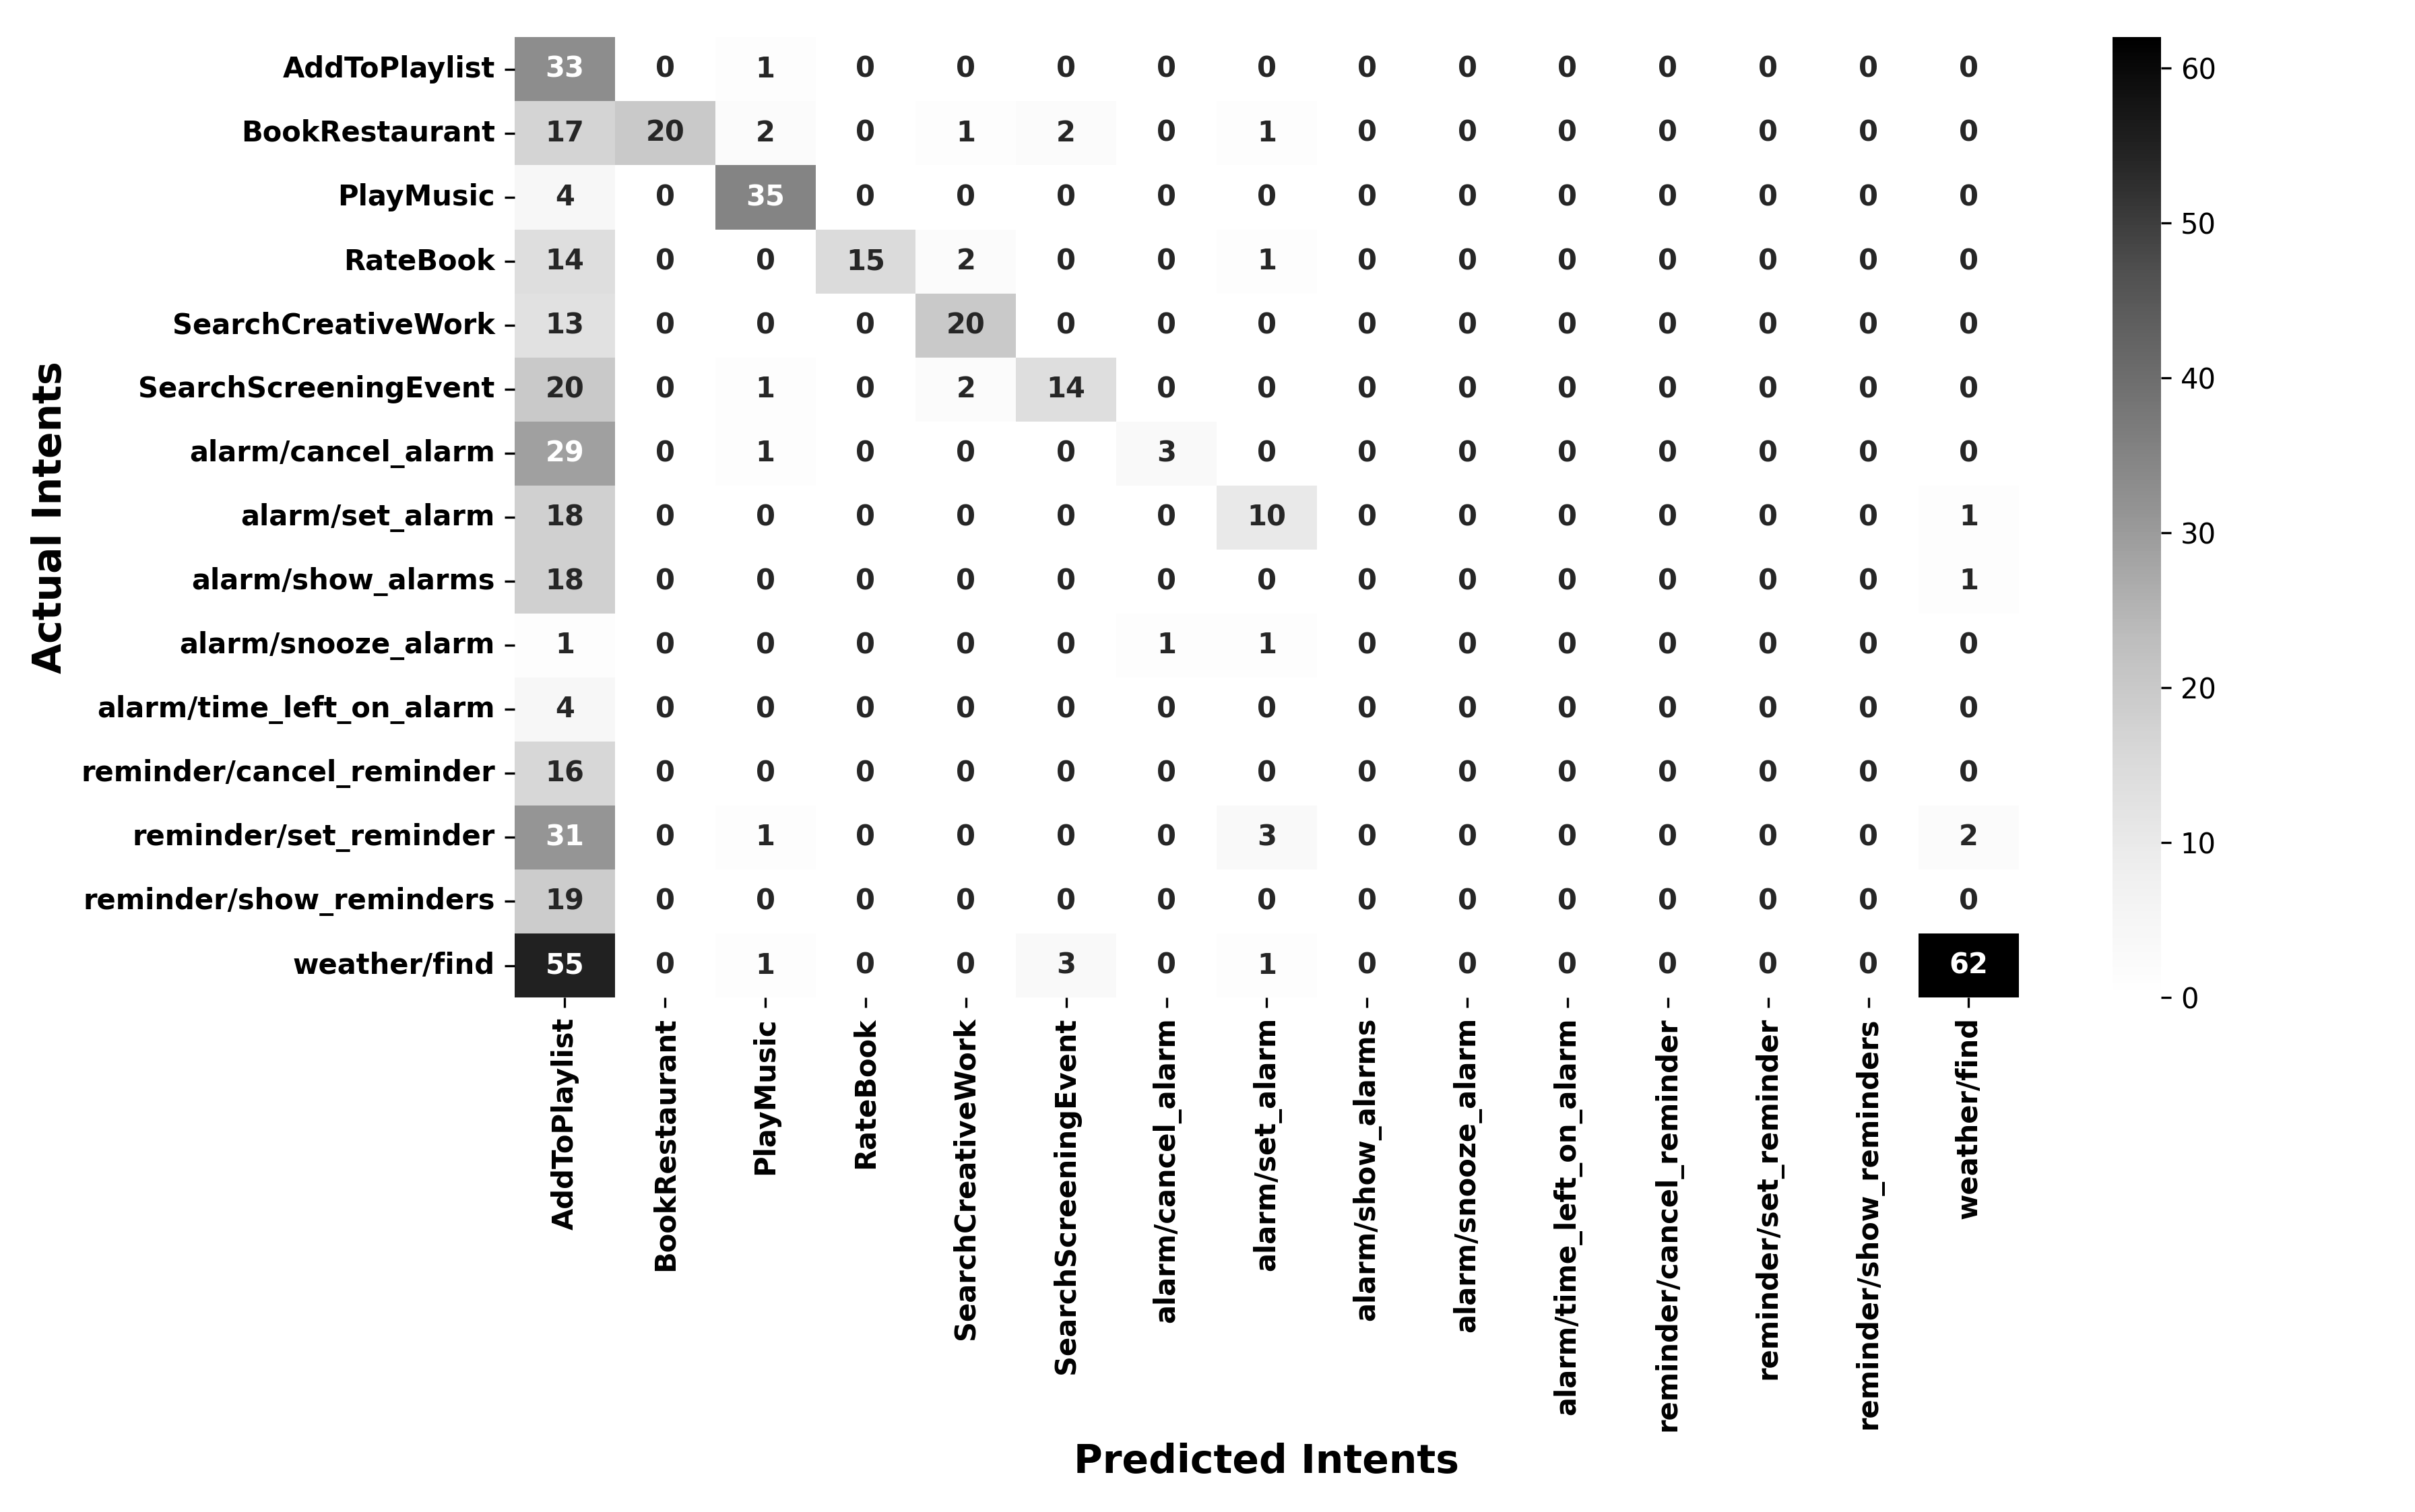
\includegraphics[width=\textwidth]{ma_figures/de-by_MLMxUDxNERxNLU.png}
    \caption{A confusion matrix for the intent classification results of a mDeBERTa model trained on MLMxUDxNERxNLU (random-seed=6543) regarding the Bavarian test set created by \citet{winkler-etal-2024-slot-intent} (de-by).}
    \label{fig:de-by_MLMxUDxNERxNLU}
\end{figure}









\subsection{Extended Sequential Intermediate Multi-Task Setting UDxNER\_NLU}

As mentioned beforehand, the final three experiments introduce a new setting which combines multi-task training on two auxiliary tasks as an intermediate task with a sequential fine-tuning of the resulting model on SID. In a first try, Table \ref{tab:mDeBERTa_exp4_udner_nlu_dialects} reveals the averaged results over mDeBERTa models being fine-tuned jointly on the tasks in the UD and NER datasets and then sequentially on the English SID data. Training this experiment is rather efficient as opposed to the previos multi-task attempts, taking one hour and twenty minutes per run. Interestingly, in the first step, similar learning curves appear for named entity slots and dependency parsing. The curve for POS tagging rises faster and to a higher maximum level, indicating a better performance for this easier sub-task. All three runs vary regarding the best epoch on the development SID data, from this being the fifteenth to the nineteenth and twentieth epoch. A clear statement on the optimal number of epochs can thus hardly be made. Regarding the results, however, two top scores are reached for intent classification on the Bavarian test set from the Munich region (de-by) and the South Tyrolean set. The average performance on Upper German dialects set does not reach the best performance due to slightly lower results on the Upper Bavarian test set. Still, this setting presents the second best attempt on intent detection. Regarding slot labelling, it ranges within the top tries as well, on a par with the best overall model that follows below. A possible explanation for this success can be the detachment between the UD tasks and SID in the fine-tuning process. It appears that here, in combination with the NER data, the models are initially fine-tuned on linguistic characteristics of Bavarian together with solving distinct and similar tasks to SID in this variety. Final training on SID data then enables the model to fully concentrate jointly on these two target tasks, adjusting the representations accordingly. This should leave the previously adjusted parameters for Bavarian task training mostly untouched.

\begin{table}[!ht]
\centering{
\begin{tabular}{l|llllll|ll}
Language      & de   & de-ba & de-by & de-st & en   & gsw  & Avg. & Diff. \\
\hline
slots         & 81.4 & 55.6  & 53.2  & 52.3  & 94.8 & 29.3 & 53.7 & 8.4   \\
intents       & 95.1 & 83.1  & \textbf{70.5}  & \textbf{81.5}  & 99.3 & 64.5 & 78.4 & 4.9   \\
fully correct & 63.1 & 25.5  & 21.1  & 20.4  & 89.9 & 7.3  & 22.3 & 7.2   \\
\hline
sd slots      & 1.3  & 1.7   & 1.6   & 0.5   & 0.7  & 0.4  &  1.2    & 0.3      \\
sd intents    & 2.7  & 1.7   & 1.8   & 1.2   & 0.2  & 3.6  &  2.2    & -0.6     
\end{tabular}}
\caption{Results for the extended sequential intermediate multi-task UDxNER\_NLU experiment with mDeBERTa according to Upper German dialects over three random seeds, Avg. = average on languages without English, German and Swiss German, Diff. = average performance difference to mDeBERTa baseline, sd = standard deviation}
\label{tab:mDeBERTa_exp4_udner_nlu_dialects}
\end{table}






\subsection{Extended Sequential Intermediate Multi-Task Setting MLMxUD\_NLU}

In order to explore whether the assumptions of the previous experiment hold true, this paragraph describes the results of a similar setting in which the intermediate task is now continuous-pre-training in combination with the UD sub-tasks POS tagging and dependency parsing. The exact results on Upper German dialects are presented in Table \ref{tab:mDeBERTa_exp4_mlmud_nlu_dialects}. Obtaining them takes one hour and forty five minutes per run, i.e. longer than for the previous experiment and additionally requiring larger resources due to MLM. As in one run the best performing model results from epoch seventeen on the development data but both others improved until the twentieth, the amount of epochs is in good range but could be enlarged. Whilst the results slightly improve for both tasks and are quite robust across three random seed runs, no exceptional numbers are reached for this rather expensive attempt. For slot labelling, however, this mid range result on the average is surprising as only POS tagging is slightly similar to this task type. Zero-shot cross-lingual transfer for intent classification is not improved over the baseline, though. It thus appears that in this setting, not enough linguistic and task knowledge is induced during the intermediate fine-tuning process to then adjust it to SID in the final model representations. This can be rooted in the small size of both training corpora of the auxiliary tasks. Increasing this would be possible for MLM but require larger computational resources.

\begin{table}[!ht]
\centering{
\begin{tabular}{l|llllll|ll}
Language      & de   & de-ba & de-by & de-st & en   & gsw  & Avg. & Diff. \\
\hline
slots         & 81.1 & 50.2  & 48.4  & 48.9  & 94.7 & 21.8 & 49.2 & 3.9   \\
intents       & 94.7 & 79.3  & 65.9  & 76.6  & 99.1 & 58.8 & 74.0 & 0.5   \\
fully correct & 61.7 & 21.2  & 18.2  & 18.5  & 89.5 & 5.3  & 19.3 & 4.2   \\
\hline
sd slots      & 0.9  & 3.3   & 2.6   & 1.8   & 0.3  & 2.2  &  2.2    &  -0.7     \\
sd intents    & 1.5  & 1.4   & 1.0   & 2.5   & 0.2  & 1.0  &  1.5    &   0.1   
\end{tabular}}
\caption{Results for the extended sequential intermediate multi-task  MLMxUD\_NLU experiment with mDeBERTa according to Upper German dialects over three random seeds, Avg. = average on languages without English, German and Swiss German, Diff. = average performance difference to mDeBERTa baseline, sd = standard deviation}
\label{tab:mDeBERTa_exp4_mlmud_nlu_dialects}
\end{table}






\subsection{Extended Sequential Intermediate Multi-Task Setting MLMxNER\_ NLU}

In a last experiment, it was aimed to overcome the possible shortcomings identified in the previous attempt by combining continuous pre-training with the larger NER set in a multi-task intermediate step before fine-tuning mDeBERTa models on SID. Although this final setting is the most time and resource intensive one, taking over two hours per random seed run, the improvements reached for both tasks as displayed in Table \ref{tab:mDeBERTa_exp4_mlmner_nlu_dialects} are worth the effort. Interestingly, the best performing final SID models upon the development data are reached after the twelfth, fifteenth and twentieth epoch in this setting. Although the results of the last epochs are close to the best numbers reached in the former two runs, this shows that the training time can actually be reduced by using less epochs. When interpreting the results, the average upon the three core Upper German dialects shows a respectable improvement for slot detection, ranging amongst the top four detected over all experiments. For intent classification, a new best result across all approaches is achieved. This is due to the highest performance on the Upper Bavarian test set which is also considerably higher as for the Munich Bavarian set. Apart from that, the best result is also reached for Swiss German intent classification. For both of these tasks, very low standard deviations are observed, lower on average than for the baseline. Thus, these results can also be classified as highly robust. Finally, a new top result is achieved for the averaged Upper German fully correct examples, closely connected to the same trend in Upper Bavarian and South Tyrolean. Similarly, the best result in this metric is gained for German. When aiming to classify these results, one can conclude that as before for UDxNER, the initial fine-tuning on two auxiliary tasks in the target language introduces dialectal characteristics and general task knowledge to the model. In this case, where NER is a task which is similar to slot detection and comes with a larger amount of tokens, this increases the intermediate training success. Additionally, concurrent MLM introduces it's strengths on intent classification, further providing the model with general knowledge on dialectal language structure and orthography. Both of these factors lead to an enhanced cross-lingual performance via zero-shot transfer learning on SID.

Finally, a closer analysis of this best intent classification transfer learning approach is made for both Bavarian datasets. Thus, Figure \ref{fig:de-ba_MLMxNER_NLU} shows the confusion matrix for the evaluation set \textit{de-ba}. It becomes apparent that now most intents are correctly predicted. Miss-classifications of one to five samples per intent are only present across some intents, going along with the top-level accuracy of 85.8. In comparison to this, the confusion matrix for the Bavarian set created in this work, \textit{de-by}, and shown in Figure \ref{fig:de-by_MLMxNER_NLU}, lets emerge a similar picture. As compared to previous figures which show that the model incorrectly classifies one intent for samples from almost all other intents, this pattern is not as predominant anymore. Still, issues for \textit{AddToPlaylist} and \textit{weather/find} exist, albeit much smaller now. More instances of miss-classifications with similarly for up to ten samples also explain the difference to \textit{de-ba}, matching the accuracy level of only 69 percent. Nevertheless, considerable improvements for intent classification can be seen by this multi-task intermediate example using MLM and NER as data and tasks.

\begin{table}[!ht]
\centering{
\begin{tabular}{l|llllll|ll}
Language      & de   & de-ba & de-by & de-st & en   & gsw  & Avg. & Diff. \\
\hline
slots         & 82.5 & 56.5  & 52.5  & 52.1  & 94.4 & 31.8 & 53.7 & 8.4   \\
intents       & 96.0 & \textbf{85.8}  & 69.0  & 81.1  & 99.1 & \textbf{69.4} & \textbf{78.6} & 5.1   \\
fully correct & \textbf{65.5} & \textbf{25.7}  & 20.5  & \textbf{22.6}  & 89.5 & 9.2  & \textbf{22.9} & 7.8   \\
\hline
sd slots      & 0.4  & 0.9   & 1.1   & 1.6   & 0.8  & 1.9  &  1.3    &  0.2     \\
sd intents    & 1.1  & 1.3   & 1.7   & 0.7   & 0.1  & 1.7  &  1.3    &  0.3    
\end{tabular}}
\caption{Results for the extended sequential intermediate multi-task MLMxNER\_NLU experiment with mDeBERTa according to Upper German dialects over three random seeds, Avg. = average on languages without English, German and Swiss German, Diff. = average performance difference to mDeBERTa baseline, sd = standard deviation}
\label{tab:mDeBERTa_exp4_mlmner_nlu_dialects}
\end{table}

% figures to show possible issues for intent detection in the Bavarian evaluatio sets
\begin{figure}[!ht]
    \centering
    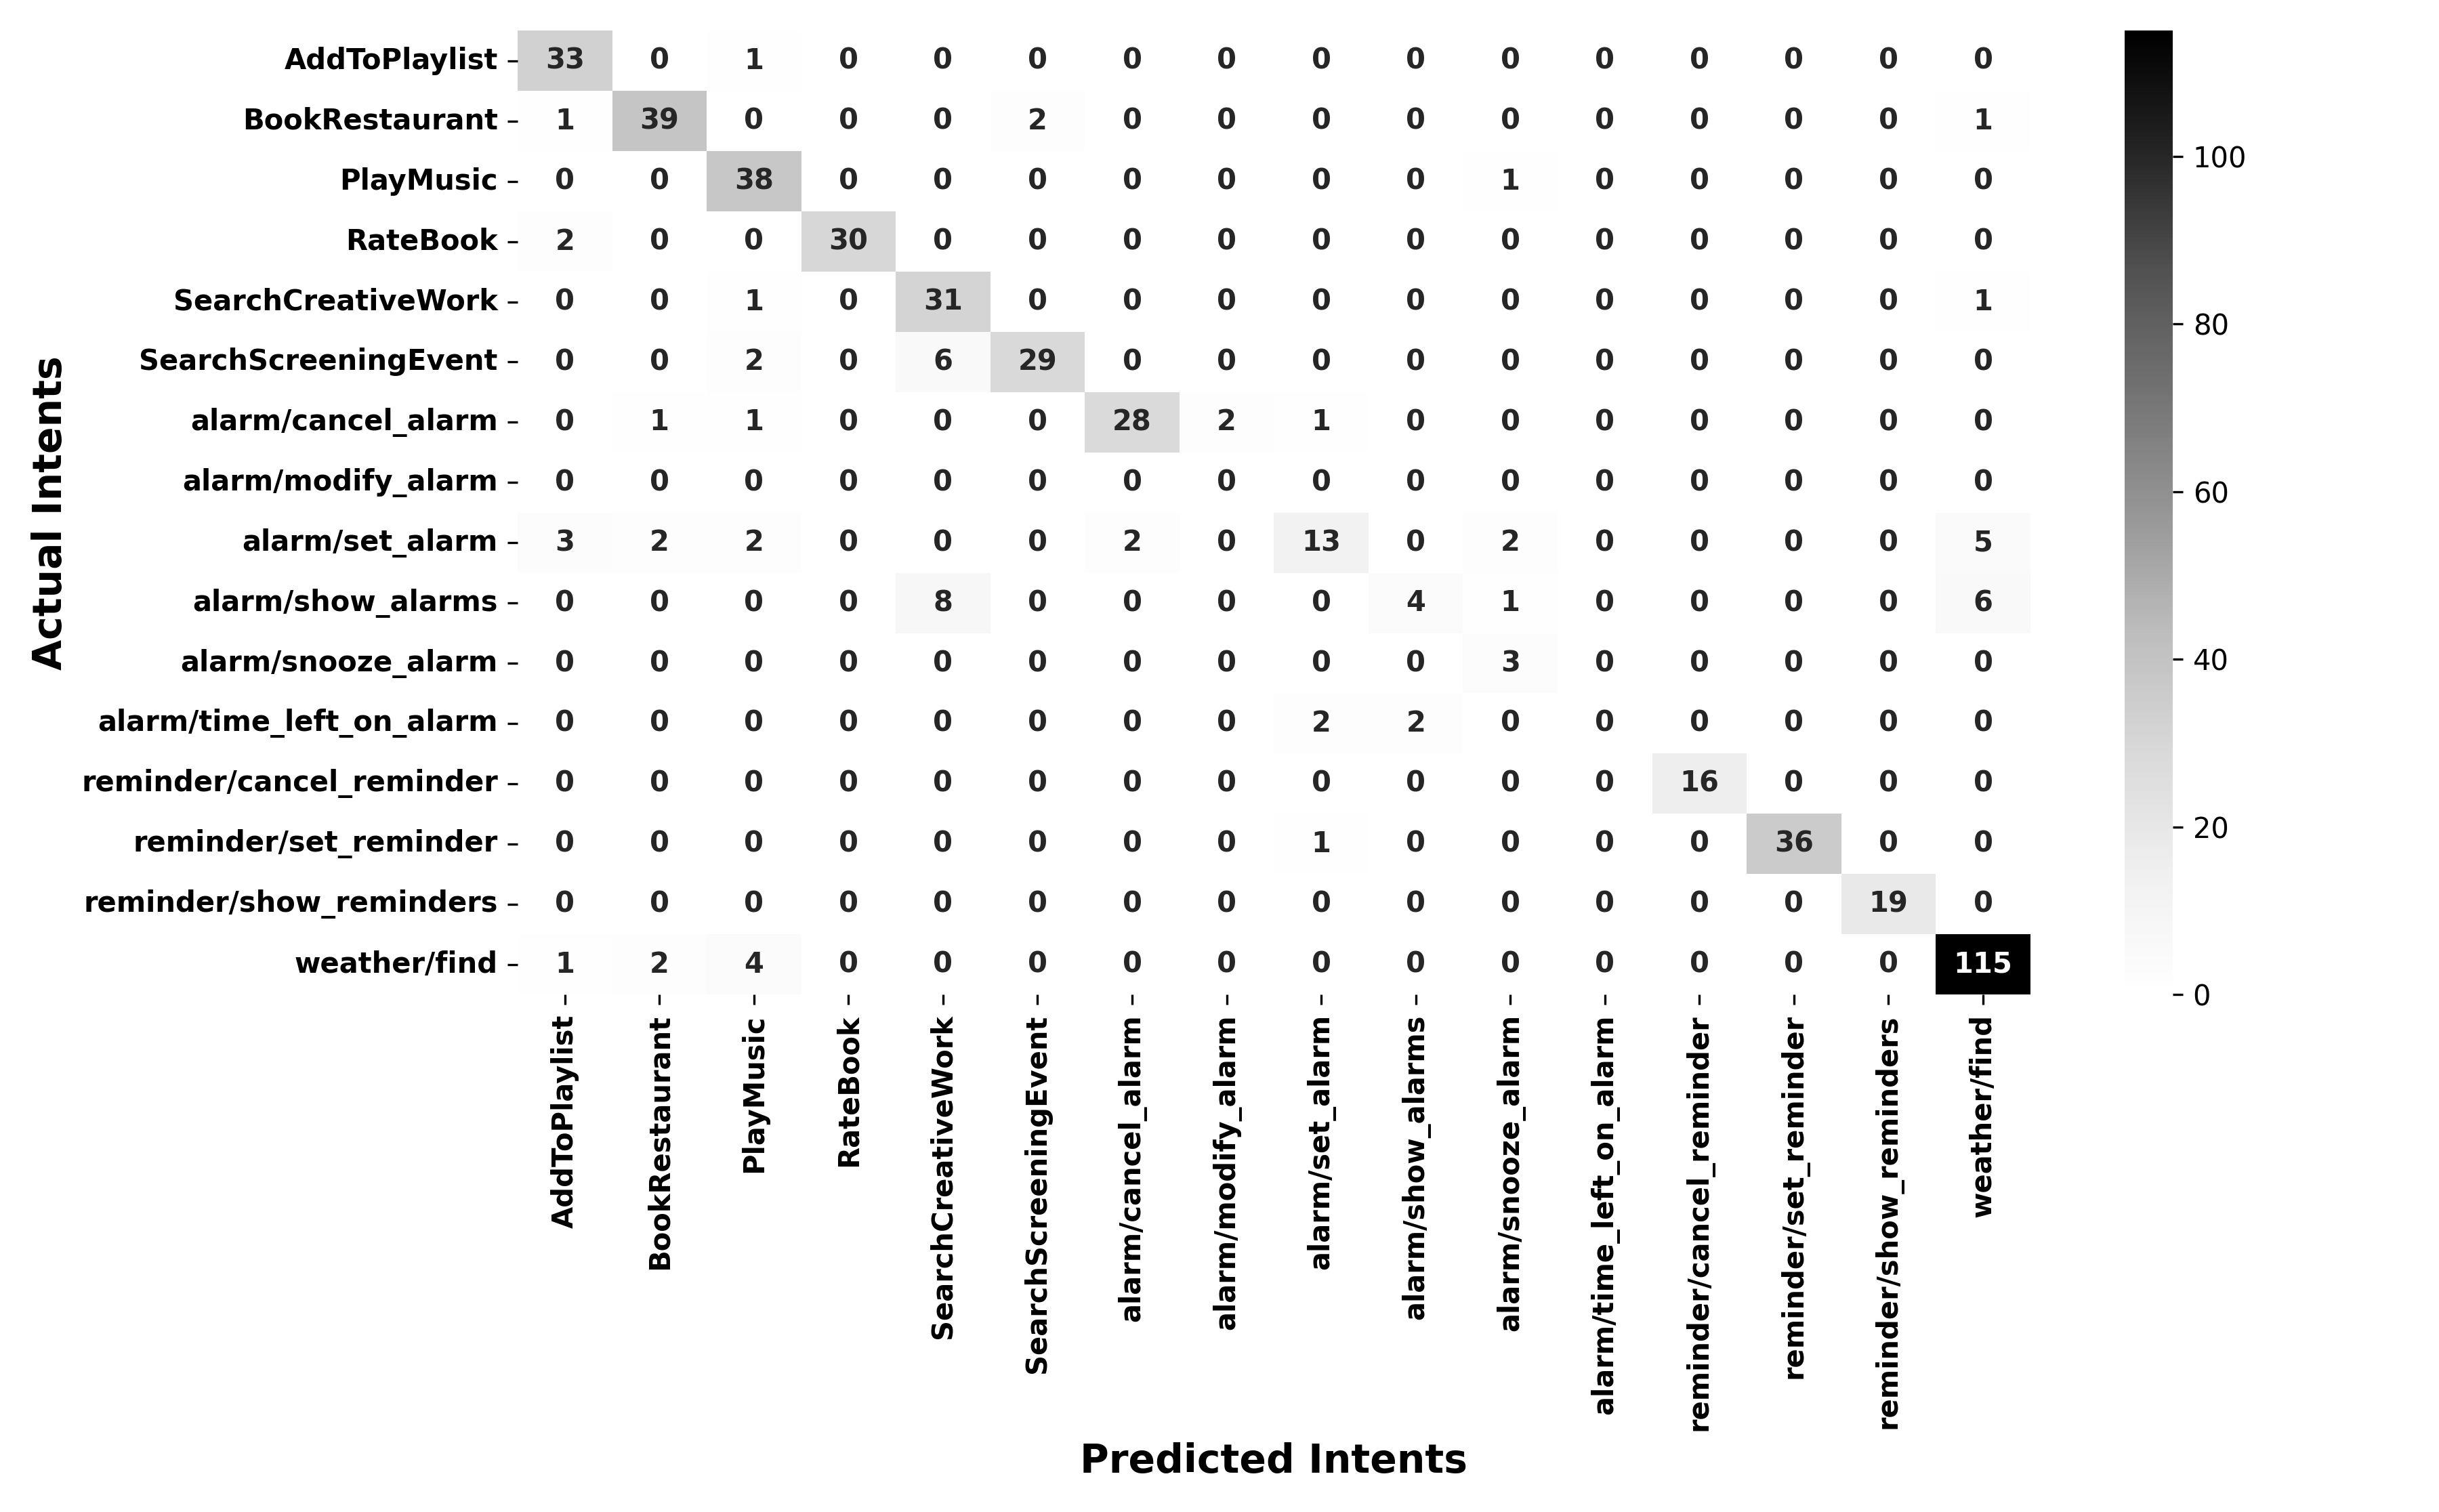
\includegraphics[width=\textwidth]{ma_figures/de-ba_MLMxNER_NLU.png}
    \caption{A confusion matrix for the intent classification results of a mDeBERTa model trained on MLMxNER\_NLU (random-seed=6543) regarding the Bavarian test set created in this work (de-ba).}
    \label{fig:de-ba_MLMxNER_NLU}
\end{figure}

\begin{figure}[!ht]
    \centering
    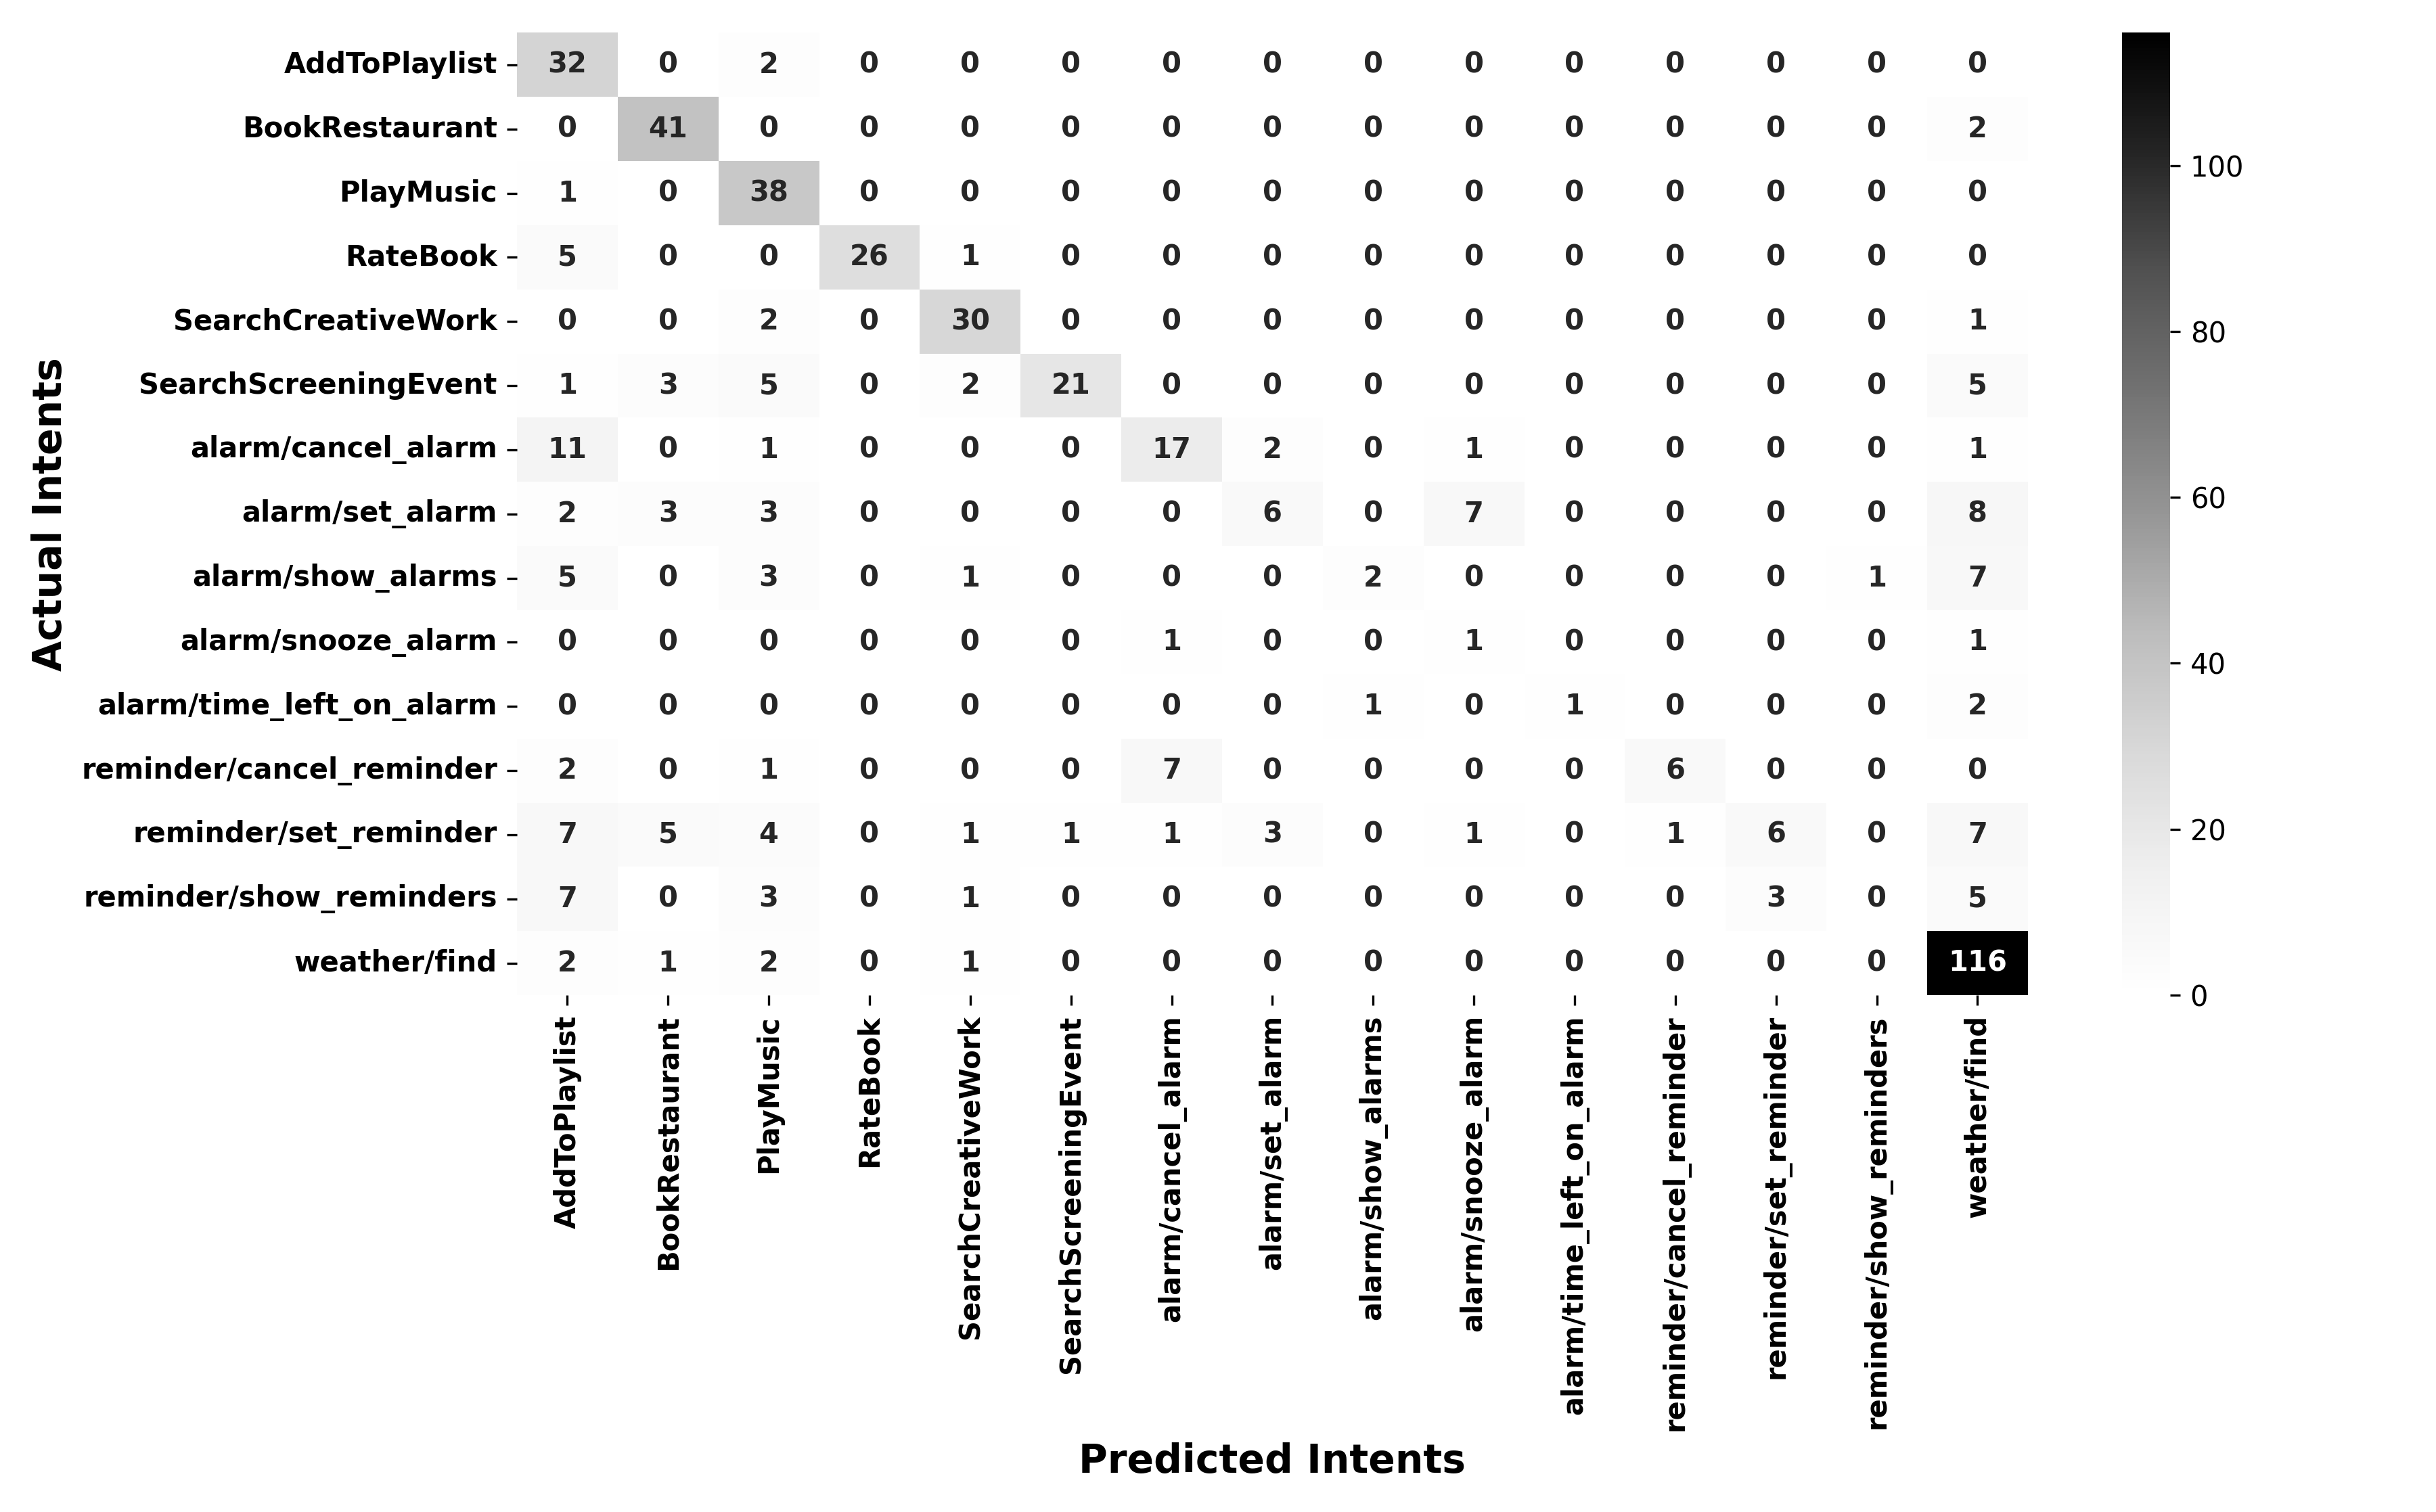
\includegraphics[width=\textwidth]{ma_figures/de-by_MLMxNER_NLU.png}
    \caption{A confusion matrix for the intent classification results of a mDeBERTa model trained on MLMxNER\_NLU (random-seed=6543) regarding the Bavarian test set created by \citet{winkler-etal-2024-slot-intent} (de-by).}
    \label{fig:de-by_MLMxNER_NLU}
\end{figure}

















\chapter{Analysis, Discussion and Future Work} 

In this second to last chapter, a comprehensive analysis of the results from both the baseline and all extended experiments is conducted within a first paragraph. In and on this, both initial research questions will be answered. A second paragraph provides additional insights, examining predicted examples from the Bavarian test set created in this work of the overall best experimental approach in comparison to the respective gold translations. In the course of this analysis, also those examples that were presented earlier as structurally different are again under observation. Similarly, the third paragraph will be related to the analysis of the best models, introducing their results on the natural Bavarian evaluation data. Subsequently, the main results are discussed in contrast to related work in this field. Finally, a last paragraph presents possible future work and fruitful adaptions to the experimental concept.






\section{A Comprehensive Analysis of Key Experimental Findings}

Regarding the baseline experiments, the consistent results of mBERT with those presented in the baseline on the same model by \citet{van-der-goot-etal-2021-masked} show that the overall procedure and approach used for this thesis is suitable for zero-shot cross-lingual transfer learning to low-resource dialects. The decent results for mBERT, an average strict F1 score of 53.6 on slot labelling and an accuracy of 71.7 over the basic xSID evaluation sets proof the model's profound multilinguality as was shown prior analyses like \citet{pires-etal-2019-multilingual} as well. However, on Upper German dialects, these numbers are around ten points lower on average over the two Bavarian and the South Tyrolean sets. Due to the training data which includes Bavarian, they are still better than for XLM-R, though. Still, this refined multilingual model based upon the BERT architecture and trained with more and more sophisticatedly chosen data shows better multilingual capabilities on the diverse xSID languages. When looking at mDeBERTa, a further multilingual model with an again improved BERT-based architecture, the average strict F1 score of 69.6 on slot labelling and an accuracy of 91.8 over the basic xSID evaluation sets indicate top level zero-shot transfer results. The numbers on the Upper German test sets are not that high but still better than for the previous models, keeping in mind that the pre-training data did not include particular dialectal texts. Finally, these results were again slightly improved by 1.9 points on slot detection by the monolingual gBERT model and thus also for the amount of fully correct results. Based on this, the reason for deciding to continue the extended experiments with mDeBERTa seems surprising at first. However, gBERT is behind this model on intent classification for dialects by 3.2 points on accuracy, although this can be seen as the easier task. Similarly, gBERT performed poorly on the diverse set of xSID evaluation languages, not even reaching half the scores on SID compared to mDeBERTa. Thus, also following the generally accepted procedure in research to fine-tune multilingual models for zero-shot cross-lingual transfer learning in low-resource settings mDeBERTa is chosen over gBERT for the extended experiments. It is expected that through multilingual pre-training, more refined adaptions regarding linguistic representations in the model's embedding space can be made which help for dialectal modelling and task-awareness. Finally, regarding the third research question, it can be said that according to the obtained numbers, the choice of the language model does make a difference regarding a transfer to a broad cross-lingual evaluation set. For a more narrow analysis like on Upper German dialects, similarly good results can be reached by a multilingual and a monolingual model with the restriction that the latter model is specially trained on text from the standard language of these dialects. If such a model is not present for even more low-resource variants, choosing a multilingual model is in fact the only option. 

When moving on to the key insights of the extended zero-shot transfer learning experiments performed with mDeBERTa on Upper German dialects that include various combinations and successions of Bavarian auxiliary task training, Table \ref{tab:overview_all_results_dialects} gives a general overview over all their results for slot labelling, intent classification and fully correct annotated samples. Starting with the basic multi-task experiments that include only one auxiliary task in a sequential or real manner, a clear picture emerges. Both sub-tasks in the UD data are not really suited to improve the results in both settings. Whilst slight slot labelling improvements are made through these being an intermediate task, combining them with SID in a real multi-task configuration downgrades the results on SID for all metrics. The main reason for this apart from the small dataset size should be the difference of task types between POS tagging plus dependency parsing and SID. In a sequential setting, this can be mitigated by the final fine-tuning step as opposed to the multi-task take. For NER as a larger dataset including a task much closer to slot labelling, both fine-tuning approaches work equally well as expected, improving the averaged results for both target tasks according to the metrics. Turning towards continuous pre-training, a similar but not as drastic picture emerges as compared to the UD experiments. Here, however, sequentially using the MLM data has more negative effects. Turning towards multi-step sequential approaches, a similar picture as just presented emerges with NER as the best intermediate task taken as the mediate task in these settings. Taking the UD tasks in a first fine-tuning step lifts the performance on slot detection on the second overall spot and similarly intent classification to a high level. In this approach, the pre-trained representations are not changed as by MLM but refined for solving tasks in the target language with rising similarity to SID. Still, the results for first performing continuous pre-training followed by NER and SID fine-tuning is also effective though time and resource intensive. It appears that MLM with Bavarian data changes model representations in a way that they are not really suitable to be adopted for solving sequence labelling and classification tasks anymore. This picture changes when MLM is part of a real multi-task setting. Together with NER and SID, this setting leads to the best overall slot detection result for zero-shot cross-lingual transfer to Upper German dialects. Similarly, intent classification and fully correct example annotation are on a high level in this attempt, rooted in the fact that by training on these closely related tasks that bring in a lot of target language linguistic knowledge, also the models ability to solve target tasks increases. However, in a setting with UD, NER and NLU, too much different task signals are handed to the base model simultaneously which leads to a decreased performance for both target tasks according to the metrics. A similar picture emerges for the multi-task setting that includes all auxiliary tasks. Though this is not bad for slot labelling, it appears to confuse the model too much for intent classification, leading to the second worst result on this task. Finally, only positive improvements can be observed for the combination of the two general settings in the last three experiments. Pairing MLM with the UD tasks as an intermediate task is the least beneficial of these, presenting too little and to diverse signals to the model which has then issues to fully capture SID. Thinks look better for the intermediate combination of UD and NER which fine-tunes the model on enough and mostly similar target language tasks. Being detached from SID training, which is also done by on the largest dataset, appears to enable the model to best adopt its representations to perform zero-shot cross-lingual transfer on SID. Especially within the last experiment, where mDeBERTa is first fine-tuned on the combination of MLM and NER data, it appears that the activation and adjustment to related task knowledge in the target language with a then following final sequential step on SID primes this for the target task by still keeping target language representations. Although slot labelling is better mastered on average by the overall multi-task setting including these auxiliary tasks, it is still amongst the top four performances. Since for intent classification and the total amount of fully correct annotated samples a new maximum is reached, this final setting presents the best overall approach in order to transfer SID in a zero-shot manner to Upper German dialects. 

\begin{table}[!ht]
\centering
\resizebox{\textwidth}{!}{
\begin{tabular}{l|cc|cc|cc}
\fontsize{12pt}{14pt}\selectfont  \textbf{Experiment}     & \textbf{Slots} & \textbf{Diff.  } & \textbf{Intents} & \textbf{Diff.  } & \textbf{Fully Correct} & \textbf{Diff.} \\
\hline
UD\_NLU        & 49.3  & 4.0         & 73.8    & 0.3           & 19.0           & 3.9                 \\
UDxNLU         & 42.1  & -3.2        & 48.9    & -24.6         & 13.0           & -2.1                \\
NER\_NLU       & 53.1  & 7.8         & 76.6    & 3.1           & 22.0           & 6.9                 \\
NERxNLU        & 53.8  & 8.5         & 76.2    & 2.7           & 21.2           & 6.1                 \\
MLM\_NLU       & 39.6  & -5.7        & 71.8    & -1.7          & 12.1           & -3.0                \\
MLMxNLU        & 44.6  & -0.7        & 71.9    & -1.6          & 14.3           & -0.8                \\
UD\_NER\_NLU   & 54.3  & 9.0         & 78.3    & 4.8           & 22.6           & 7.5                 \\
MLM\_NER\_NLU  & 51.5  & 6.2         & 76.8    & 3.3           & 21.1           & 6.0                \\
UDxNERxNLU     & 44.7  & -0.6        & 62.6    & -10.9         & 15.1           & 0.0                 \\
\textbf{MLMxNERxNLU}    & \textbf{54.8}  & \textbf{9.5}         & 77.9    & 4.4           & 22.3           & 7.3                 \\
MLMxUDxNERxNLU & 48.7  & 3.4         & 58.0    & -15.5         & 17.0           & 1.9                 \\
UDxNER\_NLU    & 53.7  & 8.4         & 78.4    & 4.9           & 22.3           & 7.2                 \\
MLMxUD\_NLU    & 49.2  & 3.9         & 74.0    & 0.5           & 19.3           & 4.2                 \\
\textbf{MLMxNER\_NLU}   & 53.7  & 8.4         & \textbf{78.6}    & \textbf{5.1}           & \textbf{22.9}           & \textbf{7.8}                 \\

\end{tabular}}
\caption{Overview over all averaged results on slot and intent detection of all experiments for Upper German dialects, i.e. the two Bavarian and the South Tyrolean test sets. Slot results are strict F1 scores, Intent and Fully Correct results are accuracy as percentage. Diff. = performance difference to the averaged mDeBERTa results on the same test sets in the baseline experiment.}
\label{tab:overview_all_results_dialects}
\end{table}







\section{Insights from Predictions on the Munich-Region Bavarian Test-Set}

This section aims to present concrete insights into the predictions of the overall best model as outlined above on the Bavarian test set created in this work, \textit{de-by}. Specifically, erroneous classifications and missing or incorrect slot labelling is under observation for this test set that depicts Bavarian as spoken in the Munich region. Generally, it has to be said that although this test set was created in a most similar way to the Upper Bavarian set by \citet{winkler-etal-2024-slot-intent} (de-ba), it always falls behind this regarding the performance of both SID tasks in all experiments. The closest result on both sets was actually reached by the baseline experiment with gBERT, in which the performance is yet only moderate, though. It rises in most of the extended experiments by adding auxiliary task data in Bavarian to the fine-tuning process. There, \textit{de-by} is always about three to five points behind regarding strict slot detection F1 scores and around almost fifteen percent in intent classification accuracy. As this is consistent across most experiments, the presented reasons of differences between the two sets made in the data chapter appear to hold true. As similarly no bigger differences on the concrete dialectal variants included in the auxiliary task data can be found, the varying performances are most likely to be rooted in a structurally and orthographically more complex annotation of \textit{de-by}.

In the following, it should thus be show for four predictions of the final experiment's model MLMxNER\_NLU on this Bavarian test set where possible difficulties lie. Therefore, the two examples which were being presented as such that differ structurally from the English gold annotation and orthographically from \textit{de-ba} are shown first. When looking at the prediction in Table \ref{tab:differences_gold_pred_bavarian1}, it is the more surprising that in this extended setting, fine-tuned mDeBERTa was able to deliver a fully correct result on this example. To remember, Tables \ref{tab:dialects_example_1} and \ref{tab:differences_bavarian} presented how this sample is annotated with a more complex structure as opposed to English and the second Bavarian test set as that more tokens need to be classified and labelled with a larger slots span. A possible reason for this is the fact that due to the tokens being numbers, it is easier for the model to detect the slot label for date-time. Moreover, the overall structure is still similar to alarm setting examples in the English training corpus. Whilst the first guess seems to hold true as can be seen in Table \ref{tab:differences_gold_pred_bavarian1.1}, the same but structurally much simpler example in \textit{de-ba} is not completely correctly annotated by the model. Thus, a similar structure to the English gold sentences is not a guarantee for a correct annotation.

Whilst for the second of these examples, already presented earlier in Tables \ref{tab:differences_gold_bavarian} and \ref{tab:dialects_example_2}, the intent for the \textit{de-by} translated sentence is still correctly classified as can be seen in Table \ref{tab:differences_gold_pred_bavarian2}, considerable issues in slot labelling occur for this complex structurally changed example. Whereas the area that includes slots was partly found at the end of the sentence down to the last token, only one slot label was chosen. This would have been correct for the last slot span but is not following the 'BIO' format and the previous slot span is not realised at all. This disturbed slot annotation can be seen as a clear indicator that the model was not able to recognize the structure and meaning of the Bavarian sentence, although it was cared for that this is as close to the English gold sample's meaning as possible. Even for the more logical translation in \textit{de-ba}, the predictions on slot spans and labels are not fully correct. As visible in \ref{tab:differences_gold_pred_bavarian2.1}, the initial slot label is found correctly but then the model just continues with this in an overall span, missing the intermediate date slot and out-of-slot tokens.

When analysing a random but much simpler example consisting just of three tokens and one slot, shown in Table \ref{tab:differences_gold_pred_bavarian3}, it becomes apparent that even in such simple and short examples, several mistakes are made by the model on the translated version in \textit{de-by}. Since the structure is clearly the same as in English here, the reason for the completely mistaken intents and two slot spans is to be rooted in the orthography or choice of words for this example. Whilst admittedly the translation of the initial token is debatable, the other two tokens are regularly translated, also in comparison to \textit{de-ba}. This can be deduced from considering Table \ref{tab:differences_gold_pred_bavarian3.1} in which the gold translation and prediction for the same simple example in \textit{de-ba }are shown. For this version, the model annotates and classifies the sample fully correct. The difference in orthography to the translation in \textit{de-by} is only marginally, though.

In a last example displayed in Table \ref{tab:differences_gold_pred_bavarian4}, it becomes apparent that the model also misses to predict any slots for \textit{de-by} in some cases. This is surprising as almost all training examples include at least one slot and especially regarding the first slot which is related to the intent, detecting is expected to be possible. Thus, this example shows that in some cases, the model has not learned close connections between intents and matching slot labels. Interestingly, the same issue happens for the prediction on the same example in \textit{de-ba} as well as can be seen in Table \ref{tab:differences_gold_pred_bavarian4.1}. This translation varies only in one token to the version in \textit{de-by} and is just a little different in structure, not carrying the temporal adverbial at sentence final position. Thus it seems to be the intent or choice of words for which the model has not encountered enough training signals for slots.


% differences between de-by gold and de-by predicted for MLMxNER\_NLU random_seed=6543
\begin{table}[!ht]
\centering
\resizebox{\textwidth}{!}{
\begin{tabular}{llll||llll}
\multicolumn{4}{l||}{\textbf{Bavarian gold (de-by):}}     & \multicolumn{4}{l}{\textbf{Bavarian predicted (de-by):}} \\
\hline
\multicolumn{4}{l||}{\# id: 156}                & \multicolumn{4}{l}{\# id: 156}            \\
\multicolumn{4}{l||}{\# text-en: Set an alarm for 6:50 pm}      & \multicolumn{4}{l}{\# text-en: Set an alarm for 6:50 pm}       \\
\multicolumn{4}{l||}{\# text: Stei an wecka fia 6:50 aufd nocht} & \multicolumn{4}{l}{\# text: Stei an wecka fia 6:50 aufd nocht} \\
\multicolumn{4}{l||}{\# intent: alarm/set\_alarm}                & \multicolumn{4}{l}{\# intent: alarm/set\_alarm}                 \\
1 & Stei      & alarm/set\_alarm & O          & 1 & Stei  & alarm/set\_alarm & O          \\
2 & an        & alarm/set\_alarm & O          & 2 & an    & alarm/set\_alarm & O          \\
3 & wecka     & alarm/set\_alarm & O          & 3 & wecka & alarm/set\_alarm & O          \\
4 & fia       & alarm/set\_alarm & O          & 4 & fia   & alarm/set\_alarm & O          \\
5 & 6         & alarm/set\_alarm & B-datetime & 5 & 6     & alarm/set\_alarm & B-datetime \\
6 & :         & alarm/set\_alarm & I-datetime & 6 & :     & alarm/set\_alarm & I-datetime \\
7 & 50        & alarm/set\_alarm & I-datetime & 7 & 50    & alarm/set\_alarm & I-datetime \\
8 & aufd      & alarm/set\_alarm & I-datetime & 8 & aufd  & alarm/set\_alarm & I-datetime \\
9 & nocht     & alarm/set\_alarm & I-datetime & 9 & nocht & alarm/set\_alarm & I-datetime
\end{tabular}}
\caption{A comparison of a previously mentioned Bavarian (de-by) gold test example and its predicted result by the mDeBERTa model trained on the setting MLMxNER\_NLU with random\_seed=6543. Being fully correct annotated, this structurally more complex example is amongst the 20.4 percent that were completely correct predicted in this run. (The average on all runs is 20.5 percent correct examples for this setting)}
\label{tab:differences_gold_pred_bavarian1}
\end{table}

% differences between de-ba gold and de-ba predicted for MLMxNER\_NLU random_seed=6543
\begin{table}[!ht]
\centering
\resizebox{\textwidth}{!}{
\begin{tabular}{llll||llll}
\multicolumn{4}{l||}{\textbf{Bavarian gold (de-ba):}}     & \multicolumn{4}{l}{\textbf{Bavarian predicted (de-ba):}} \\
\hline
\multicolumn{4}{l||}{\# id: 155}                & \multicolumn{4}{l}{\# id: 154}            \\
\multicolumn{4}{l||}{\# text-en: Set an alarm for 6:50 pm}      & \multicolumn{4}{l}{\# text-en: Set an alarm for 6:50 pm}       \\
\multicolumn{4}{l||}{\# text: Setz an Wegga füa 6:50 nammiddog} & \multicolumn{4}{l}{\# text: Setz an Wegga füa 6:50 nammiddog} \\
\multicolumn{4}{l||}{\# intent: alarm/set\_alarm}                & \multicolumn{4}{l}{\# intent: alarm/set\_alarm}                 \\
1 & Setz      & alarm/set\_alarm & O          & 1 & Setz        & alarm/set\_alarm & O          \\
2 & an        & alarm/set\_alarm & O          & 2 & an          & alarm/set\_alarm & O          \\
3 & Wegga     & alarm/set\_alarm & O          & 3 & Wegga       & alarm/set\_alarm & O          \\
4 & füa       & alarm/set\_alarm & O          & 4 & füa         & alarm/set\_alarm & O          \\
5 & 6:50      & alarm/set\_alarm & B-datetime & 5 & 6:50        & alarm/set\_alarm & B-datetime \\
6 & nammiddog & alarm/set\_alarm & I-datetime & 6 & nammiddog   & alarm/set\_alarm & O 
\end{tabular}}
\caption{A comparison of a previously mentioned Bavarian (de-ba) gold test example and its predicted result by the mDeBERTa model trained on the setting MLMxNER\_NLU with random\_seed=6543. In fact, this is the respective parallel example to the one for \textit{de-by} presented in Table \ref{tab:differences_gold_pred_bavarian1}. Whilst the intent is still correctly annotated, the final slot label is missing in the model's prediction although this example is structurally much closer to the English gold annotation.}
\label{tab:differences_gold_pred_bavarian1.1}
\end{table}


% differences between de-by gold and de-by predicted for MLMxNER\_NLU random_seed=6543
\begin{table}[!ht]
\centering
\resizebox{\textwidth}{!}{
\begin{tabular}{llll||llll}
\multicolumn{4}{l||}{\textbf{Bavarian gold (de-by):}}     & \multicolumn{4}{l}{\textbf{Bavarian predicted (de-by):}} \\
\hline
\multicolumn{4}{l||}{\# id: 92}                & \multicolumn{4}{l}{\# id: 92}            \\
\multicolumn{4}{l||}{\# text-en: remind me to set alarms for morning}      & \multicolumn{4}{l}{\# text-en: remind me to set alarms for morning}       \\
\multicolumn{4}{l||}{\# text: erinnad mi dass i fia in da fria wecka stei} & \multicolumn{4}{l}{\# text: erinnad mi dass i fia in da fria wecka stei} \\
\multicolumn{4}{l||}{\# intent: reminder/set\_reminder}                & \multicolumn{4}{l}{\# intent: reminder/set\_reminder}   \\
1 & erinnad   & reminder/set\_reminder & O                  & 1  & erinnad  & reminder/set\_reminder & O          \\
2 & mi        & reminder/set\_reminder & O                  & 2  & mi       & reminder/set\_reminder & O          \\
3 & dass      & reminder/set\_reminder & O                  & 3  & dass     & reminder/set\_reminder & O          \\
4 & i         & reminder/set\_reminder & O                  & 4  & i        & reminder/set\_reminder & O          \\
5 & fia       & reminder/set\_reminder & O                  & 5  & fia      & reminder/set\_reminder & O           \\
6 & in        & reminder/set\_reminder & B-datetime         & 6  & in       & reminder/set\_reminder & I-reminder/todo \\
7 & da        & reminder/set\_reminder & I-datetime         & 7  & da       & reminder/set\_reminder & I-reminder/todo \\
8 & fria      & reminder/set\_reminder & I-datetime         & 8  & fria     & reminder/set\_reminder & I-reminder/todo \\
9 & wecka     & reminder/set\_reminder & B-reminder/todo    & 9  & wecka    & reminder/set\_reminder & I-reminder/todo \\
10 & stei     & reminder/set\_reminder & I-reminder/todo    & 10 & stei     & reminder/set\_reminder & O
\end{tabular}}
\caption{A comparison of a previously mentioned Bavarian (de-by) gold test example and its predicted result by the mDeBERTa model trained on the setting MLMxNER\_NLU with random\_seed=6543. Whilst having detected the intent correctly, this example reveals considerable issues for slot labelling for a structurally different to the English gold annotation and thus to the structure used in the English SID training set.}
\label{tab:differences_gold_pred_bavarian2}
\end{table}

% differences between de-ba gold and de-ba predicted for MLMxNER\_NLU random_seed=6543
\begin{table}[!ht]
\centering
\resizebox{\textwidth}{!}{
\begin{tabular}{llll||llll}
\multicolumn{4}{l||}{\textbf{Bavarian gold (de-ba):}}     & \multicolumn{4}{l}{\textbf{Bavarian predicted (de-ba):}} \\
\hline
\multicolumn{4}{l||}{\# id: 92}                & \multicolumn{4}{l}{\# id: 92}            \\
\multicolumn{4}{l||}{\# text-en: remind me to set alarms for morning}      & \multicolumn{4}{l}{\# text-en: remind me to set alarms for morning}       \\
\multicolumn{4}{l||}{\# text: Erinner mi Wegga für moang zum stein} & \multicolumn{4}{l}{\# text: Erinner mi Wegga für moang zum stein} \\
\multicolumn{4}{l||}{\# intent: reminder/set\_reminder}                & \multicolumn{4}{l}{\# intent: reminder/set\_reminder}   \\
1 & Erinner   & reminder/set\_reminder & O                  & 1  & Erinner  & reminder/set\_reminder & O          \\
2 & mi        & reminder/set\_reminder & O                  & 2  & mi       & reminder/set\_reminder & O          \\
3 & Wegga     & reminder/set\_reminder & B-reminder/todo    & 3  & Wegga    & reminder/set\_reminder & B-reminder/todo  \\
4 & füa       & reminder/set\_reminder & O                  & 4  & füa      & reminder/set\_reminder & I-reminder/todo \\
5 & moang     & reminder/set\_reminder & B-datetime         & 5  & moang    & reminder/set\_reminder & I-reminder/todo \\
6 & zum       & reminder/set\_reminder & O                  & 6  & zum      & reminder/set\_reminder & I-reminder/todo \\
7 & stein     & reminder/set\_reminder & B-reminder/todo    & 7  & stein    & reminder/set\_reminder & I-reminder/todo 
\end{tabular}}
\caption{A comparison of a previously mentioned Bavarian (de-ba) gold test example and its predicted result by the mDeBERTa model trained on the setting MLMxNER\_NLU with random\_seed=6543. In fact, this is the respective parallel example to the one for \textit{de-by} presented in Table \ref{tab:differences_gold_pred_bavarian2}. Whilst the intent is still correctly annotated again, the slot spans and one label are not correctly found. The prediction starts with the correct label but then just continues a span with this.}
\label{tab:differences_gold_pred_bavarian2.1}
\end{table}


% differences between de-by gold and de-by predicted for MLMxNER\_NLU random_seed=6543
\begin{table}[!ht]
\centering
\resizebox{\textwidth}{!}{
\begin{tabular}{llll||llll}
\multicolumn{4}{l||}{\textbf{Bavarian gold (de-by):}}     & \multicolumn{4}{l}{\textbf{Bavarian predicted (de-by):}} \\
\hline
\multicolumn{4}{l||}{\# id: 93}                & \multicolumn{4}{l}{\# id: 93}            \\
\multicolumn{4}{l||}{\# text-en: delete all alarms}      & \multicolumn{4}{l}{\# text-en: delete all alarms}       \\
\multicolumn{4}{l||}{\# text: streich olle wecka} & \multicolumn{4}{l}{\# text: streich olle wecka} \\
\multicolumn{4}{l||}{\# intent: alarm/cancel\_alarm}                & \multicolumn{4}{l}{\# intent: AddToPlaylist}   \\
1 & streich   & alarm/cancel\_alarm & O                  & 1  & streich  & alarm/cancel\_alarm & B-entity\_name          \\
2 & olle      & alarm/cancel\_alarm & B-reference        & 2  & olle     & alarm/cancel\_alarm & I-reminder/todo          \\
3 & wecka     & alarm/cancel\_alarm & O                  & 3  & wecka    & alarm/cancel\_alarm & O          
\end{tabular}}
\caption{A comparison of a random Bavarian (de-by) gold test example and its predicted result by the mDeBERTa model trained on the setting MLMxNER\_NLU with random\_seed=6543. In this rather simple example, neither detecting the intent nor the slot was achieved correctly.}
\label{tab:differences_gold_pred_bavarian3}
\end{table}

% differences between de-ba gold and de-ba predicted for MLMxNER\_NLU random_seed=6543
\begin{table}[!ht]
\centering
\resizebox{\textwidth}{!}{
\begin{tabular}{llll||llll}
\multicolumn{4}{l||}{\textbf{Bavarian gold (de-ba):}}     & \multicolumn{4}{l}{\textbf{Bavarian predicted (de-ba):}} \\
\hline
\multicolumn{4}{l||}{\# id: 93}                & \multicolumn{4}{l}{\# id: 93}            \\
\multicolumn{4}{l||}{\# text-en: delete all alarms}      & \multicolumn{4}{l}{\# text-en: delete all alarms}       \\
\multicolumn{4}{l||}{\# text: Lösch alle Wegga} & \multicolumn{4}{l}{\# text: Lösch alle Wegga} \\
\multicolumn{4}{l||}{\# intent: alarm/cancel\_alarm}                & \multicolumn{4}{l}{\# intent: alarm/cancel\_alarm}   \\
1 & Lösch     & alarm/cancel\_alarm & O                  & 1  & Lösch    & alarm/cancel\_alarm & O          \\
2 & alle      & alarm/cancel\_alarm & B-reference        & 2  & alle     & alarm/cancel\_alarm & B-reference         \\
3 & Wegga     & alarm/cancel\_alarm & O                  & 3  & Wegga    & alarm/cancel\_alarm & O          
\end{tabular}}
\caption{A comparison of the same random Bavarian (de-ba) gold test example and its predicted result by the mDeBERTa model trained on the setting MLMxNER\_NLU with random\_seed=6543 as in Table \ref{tab:differences_gold_pred_bavarian3}. For the translation of this example, both detecting the intent and the slot was achieved correctly.}
\label{tab:differences_gold_pred_bavarian3.1}
\end{table}


% differences between de-by gold and de-by predicted for MLMxNER\_NLU random_seed=6543
\begin{table}[!ht]
\centering
\resizebox{\textwidth}{!}{
\begin{tabular}{llll||llll}
\multicolumn{4}{l||}{\textbf{Bavarian gold (de-by):}}     & \multicolumn{4}{l}{\textbf{Bavarian predicted (de-by):}} \\
\hline
\multicolumn{4}{l||}{\# id: 91}                & \multicolumn{4}{l}{\# id: 91}            \\
\multicolumn{4}{l||}{\# text-en: How hot will it get today?}      & \multicolumn{4}{l}{\# text-en: How hot will it get today?}       \\
\multicolumn{4}{l||}{\# text: Wia hoaß werds heid wern?} & \multicolumn{4}{l}{\# text: Wia hoaß werds heid wern?} \\
\multicolumn{4}{l||}{\# intent: weather/find}                & \multicolumn{4}{l}{\# intent: weather/find}                 \\
1 & Wia       & weather/find & O                    & 1 & Wia   & weather/find & O          \\
2 & hoaß      & weather/find & B-weather/attribute  & 2 & hoaß  & weather/find & O          \\
3 & werds     & weather/find & O                    & 3 & werds & weather/find & O          \\
4 & heid      & weather/find & B-datetime           & 4 & heid  & weather/find & O          \\
5 & wern      & weather/find & O                    & 5 & wern  & weather/find & O            \\
6 & ?         & weather/find & O                    & 6 & ?     & weather/find & O 
\end{tabular}}
\caption{A comparison of a random Bavarian (de-by) gold test example and its predicted result by the mDeBERTa model trained on the setting MLMxNER\_NLU with random\_seed=6543. Whilst having detected the intent correctly, this example reveals considerable issues for slot labelling regarding not having detected any of the two slots in this example.}
\label{tab:differences_gold_pred_bavarian4}
\end{table}

% differences between de-by gold and de-by predicted for MLMxNER\_NLU random_seed=6543
\begin{table}[!ht]
\centering
\resizebox{\textwidth}{!}{
\begin{tabular}{llll||llll}
\multicolumn{4}{l||}{\textbf{Bavarian gold (de-ba):}}     & \multicolumn{4}{l}{\textbf{Bavarian predicted (de-ba):}} \\
\hline
\multicolumn{4}{l||}{\# id: 91}                & \multicolumn{4}{l}{\# id: 91}            \\
\multicolumn{4}{l||}{\# text-en: How hot will it get today?}      & \multicolumn{4}{l}{\# text-en: How hot will it get today?}       \\
\multicolumn{4}{l||}{\# text: Wia hoaß wirds heid?} & \multicolumn{4}{l}{\# text: Wia hoaß wirds heid?} \\
\multicolumn{4}{l||}{\# intent: weather/find}                & \multicolumn{4}{l}{\# intent: weather/find}                 \\
1 & Wia       & weather/find & O                    & 1 & Wia   & weather/find & O          \\
2 & hoaß      & weather/find & B-weather/attribute  & 2 & hoaß  & weather/find & O          \\
3 & wirds     & weather/find & O                    & 3 & wirds & weather/find & O          \\
4 & heid      & weather/find & B-datetime           & 4 & heid  & weather/find & O          \\
5 & ?         & weather/find & O                    & 5 & ?     & weather/find & O 
\end{tabular}}
\caption{A comparison of the same random Bavarian (de-ba) gold test example and its predicted result by the mDeBERTa model trained on the setting MLMxNER\_NLU with random\_seed=6543 as in Table \ref{tab:differences_gold_pred_bavarian4}. For the translation of this example, detecting the intent was correct but none of the two slots were recognized correctly.}
\label{tab:differences_gold_pred_bavarian4.1}
\end{table}




\section{Performance of Top SID Approaches on Natural Bavarian Evaluation Data}

Having encountered various differences in predicted annotations for both Bavarian evaluation sets, it suggests itself to test this model's performance on the natural Bavarian evaluation data provided by \citet{winkler-etal-2024-slot-intent}, presented in more detail within the data chapter above. At first, in order to be able to classify these results, Table \ref{tab:baseline_natural_results} shows the results of the natural data on the baseline models. Interestingly, the results on the Bavarian test set which is only based upon natural utterances from native speakers (de-ba-nat) performs best for both slot and intent detection as well as on the fully correct annotated examples, of course. As opposed to the baseline performance on the two Bavarian xSID translated evaluation sets, however, the result is far behind. This becomes even more clear when combining the results on the \textit{de-ba-MAS} set. The findings on this large similarly translated set are even poorer. Since these rise in combination with the \textit{de-ba} test set in \textit{de-ba-xMAS}, it can clearly be said that this is due to the different sample structure, meaning and other factors that differentiate the cleaned xSID examples from those taken and translated in their raw shape from the MASSIVE corpus.

When analysing the numbers of the natural sets evaluated for the auxiliary task fine-tuned model which provided the best result for slot detection, MLMxNERxNLU, a similar improvement becomes visible in Table \ref{tab:mlmxnerxnlu_natural_results}. The strict slot labelling F1 score rises by over 10 points on the natural evaluation set. Similar trends are visible for the two other, larger sets and on average. However, no improvement and in fact an averaged slight decrease is visible for intent detection over all sets, a considerable difference to the xSID data which would be even stronger if this data was not present in \textit{de-ba-xMAS}. Based on this low performance, the amount of fully correct annotated examples also drops. 
Table \ref{tab:mlmxner_nlu_natural_results} finally shows the results of natural data being evaluated on the best intent classification approach, MLMxNER\_NLU. As expected, the performance on this task increases for all three datasets. The trend is even larger than on the Upper German xSID evaluation sets. However, what is even more interesting is the fact that for the models trained on this multi-task intermediate setting, also the results on slot detection are almost on par with those reached by the slot-specific approach before. Thus, on average, this final attempt provides clearly the best setting on SID for natural Bavarian utterances.

\begin{table}[!ht]
\centering{
\begin{tabular}{l|lll|l}
Evaluation Set & de-ba-nat & de-ba-MAS & de-ba-xMAS & Avg. \\
\hline
slots          & 31.7      & 22.1      & 30.3       & 28.0 \\
intents        & 60.8      & 55.2      & 60.3       & 58.8 \\
fully correct  & 12.9      & 6.7       & 9.1        & 9.6  \\
\hline
sd slots       & 2.3       & 1.4       & 0.9        & 1.5     \\
sd intents     & 1.4       & 3.5       & 1.0        & 2.0    
\end{tabular}}
\caption{Overview of the averaged results for the natural Bavarian evaluation datasets provided by the mDeBERTa baseline models trained on three different random seeds. Avg. is the average over all three datasets, sd = standard deviation.}
\label{tab:baseline_natural_results}
\end{table}

\begin{table}[!ht]
\centering{
\begin{tabular}{l|lll|ll}
Evaluation Set & de-ba-nat & de-ba-MAS & de-ba-xMAS & Avg. & Diff. \\
\hline
slots          & 42.3      & 30.3      & 39.7       & 37.4 & 9.4   \\
intents        & 61.0      & 53.8      & 60.8       & 58.5 & -0.3  \\
fully correct  & 20.3      & 10.6      & 14.9       & 15.3 & 5.7   \\
\hline
sd slots       & 2.1       & 0.9       & 0.7        &  1.2    &  0.3     \\
sd intents     & 3.9       & 2.5       & 1.7        &  2.8    &  -0.8    
\end{tabular}%
}
\caption{Overview of the averaged results for the natural Bavarian evaluation datasets provided by the mDeBERTa MLMxNERxNLU models trained on three different random seeds. Avg. is the average over all three datasets, Diff. is the difference to the average performance of the natural data on mDeBERTa baseline, sd = standard deviation.}
\label{tab:mlmxnerxnlu_natural_results}
\end{table}

\begin{table}[!ht]
\centering{
\begin{tabular}{l|lll|ll}
Evaluation Set & de-ba-nat & de-ba-MAS & de-ba-xMAS & Avg. & Diff. \\
\hline
slots          & 41.4      & 32.0      & 39.8       & 37.7 & 9.7   \\
intents        & 67.5      & 60.1      & 66.2       & 64.6 & 5.8   \\
fully correct  & 20.2      & 12.4      & 16.1       & 16.2 & 6.6   \\
\hline
sd slots       & 2.5       & 1.4       & 1.1        &  1.7    &   -0.2    \\
sd intents     & 1.3       & 1.2       & 0.3        &  0.9    &    1.1  
\end{tabular}}
\caption{Overview of the averaged results for the natural Bavarian evaluation datasets provided by the mDeBERTa MLMxNER\_NLU models trained on three different random seeds. Avg. is the average over all three datasets, Diff. is the difference to the average performance of the natural data on mDeBERTa baseline, sd = standard deviation.}
\label{tab:mlmxner_nlu_natural_results}
\end{table}






\section{A Broad Discussion of Main Results Regarding Related Work}

This section aims to discuss the main results of this thesis in the light of related work. Overall, it can be said that using the model approach of \citet{van-der-goot-etal-2021-masked} to introduce auxiliary tasks in the target language or rather language variety helps to improve zero-shot cross-lingual transfer to other (low-resource) languages and dialects. However, based on the kind and amount of auxiliary task data available in Bavarian as a target dialect, not all of the approaches in \citet{van-der-goot-etal-2021-masked} could be carried out or performed on a reasonable amount of data. Thus, the finding of UD data leading to a performance increase in cases where Bavarian is not seen during pre-training cannot fully be supported here. Both tasks which are annotated in the small Bavarian UD set used here seem to rather intimidate the model as they only really help in scenarios where they were not part in a real multi-task setting. The same applies to MLM which could not be performed in a reasonable scope here and thus, instead of leading to most stable improvements in performance as reported by \citet{van-der-goot-etal-2021-masked}, rather impaired the final results. However, the authors also state that MLM is only viable when enough training time and computational resources are available. Regarding Upper German dialects, the authors show that using a small amount of South Tyrolean, a dialect which they find not being present in multilingual embeddings, MLM increased the performance on both tasks. The amount of text that was scraped for this is still considerably more than was used here for Bavarian. Due to missing resources on parallel data to integrate experiments using machine translation as data augmentation, this approach which especially outperformed all other proposed settings in \citet{van-der-goot-etal-2021-masked} could not be tried out. On slot detection, though, this method also has drawbacks. An issue that is present throughout all attempts being made to reason the performance of different settings is the fact that probably in all models, differences between the pre-trained features and those necessary for the target domain exist \citep{hedderich-etal-2021-survey}. This becomes most visible in the actually good results provided by gBERT. In as far these would improve by using auxiliary tasks is doubtful as the model is primarily trained on German text. The model's drawbacks on the diverse set of xSID evaluation languages needs to be considered even when the target is just Upper German dialects. \citet{xu-etal-2020-end} state this as a main factor to illustrate possible strengths and weaknesses for models being used in cross-lingual transfer learning settings. Finally fine-tuning BERT with character level noise for zero-shot transfer could have increased the performance on Upper German dialects as well, following \citet{srivastava-chiang-2023-fine} and a more enhanced version of introducing noise to BERT via using noise-trained encoder layers in the stack of the architecture \citep{srivastava-chiang-2023-bertwich}. This latter work has shown to effectively reduce the embedding space between regular and noisy tokens and is thus especially useful in transfer-learning settings to dialectal variants. In the present work, it can be argued that at least word-level noise in the sense of different orthographies was introduced via Bavarian target task data. Thus, this should have made a similar impact during model training. The second option \citet{srivastava-chiang-2023-fine} use, namely including linguistic or task data from unrelated languages is also partly done here when the results of transfer learning are analysed for those dialects that are not Bavarian. Since for these a similar performance increase could be found, this option is also viable.






\section{A Final Presentation of Future Work and Potential Conceptual Adaptions}

This last section aims to provide an overview on possible future work on zero-shot cross-lingual transfer learning for SID to Upper German dialects and similar varieties in general. Thus, this will present potential conceptual adaptions that are similarly based upon concepts from related work. At first, a different approach that can be used in order to enhance slot labelling in cases where domains are present in the sufficiently available high-resource training data but not in the low-resource target language is developed by \citet{razumovskaia-etal-2023-transfer}. This work, based on turning multilingual standard sentence encoders into independent slot labelers, makes performing zero-shot transfer learning unnecessary, though. The authors argument that their transfer-free process is in fact more natural since English high-resource slots are not always similar to the slots and spans in the target languages. Slot labelling in such scenarios can, however, also be improved by using task specific models instead of, as presented, multilingual models \citep{louvan-magnini-2020-recent}. Such embeddings contain advanced task-specific representations of which knowledge on NER and additional semantic features is especially beneficial for slot filling. In order to improve cross-lingual transfer learning for sentence classification and thus for intent detection, \citet{liu-etal-2023-crosslingual-transfer} present an approach that makes use of multilingual colexification, a phenomenon that describes the condition in which one lexical form conveys more than one lexical meanings. Introducing this knowledge could be especially useful in dialectal circumstances where often synonymous terms are used as in the example given in Tables \ref{tab:differences_gold_pred_bavarian3} and \ref{tab:differences_gold_pred_bavarian3.1}. Another option for future work that could be implemented more easily is to use a non-English development set as proposed by \citet{keung-etal-2020-dont}. However, \citet{van-der-goot-etal-2021-masked} also state that then, no clear zero-shot transfer learning is done anymore when this is a collection of the target languages. Thus, this option could only help in circumstances where sufficient development data is available and using zero-shot methods is not required. 

A whole new paragraph is appropriate to present the amount of using data augmentation techniques in future work in order to improve zero-shot transfer learning to dialects. Apart from learning on SID, this has been investigated qualitatively and quantitatively for dialectal NER by \citet{peng-etal-2024-sebastian-basti}. Beyond that, both works in \citet{2023-findings-vardial}, i.e. \citet{kwon-etal-2023-sidlr} and \citet{srivastava-chiang-2023-fine} have shown to reach higher performances on South Tyrolean and Swiss German by using the given datasets which include translations from English to other high resource languages. A further multi-sentence data augmentation method that can be combined with layer aggregation procedures as presented by \citet{razumovskaia-etal-2022-data} could be used in future work on this topic. Additional training data, though mostly for few-shot settings, is collected and automatically labelled from monolingual corpora. The latter method helps in selecting and combining the most useful information across the layers of BERT-based transformer models and is thus suitable for zero-shot learning. Using more training data has been shown to be beneficial in works on the MASSIVE dataset by \citet{fitzgerald-etal-2023-massive} and \citet{jhan-etal-2022-c5l7}. Still, slot filling appears as the harder task in these transfer learning settings, resulting from lower performances on German, for example. Similarly, augmenting the training data via machine translation based on a generated parallel corpus boosted the results on SID significantly, especially when a multilingual training corpus was chosen \citep{jhan-etal-2022-c5l7}. Using neural machine translation to train a multilingual model has also been shown to be useful for settings with language variants as the model has learned patterns from the languages used during training \citep{Zampieri_Nakov_Scherrer_2020}. However, these benefits can partly be rooted in the sharing of sub-word vocabularies, allowing the model to learn spelling as well as morphological variations. Although machine translation data is lacking for Upper German dialects, sets from German or other Germanic languages could help and be tried out in future work. However, there is also critical voices that assign machine translated augmentation data a lack of natural language style and cultural specificity \citep{majewska-etal-2023-cross}. Thus, these authors propose a different annotation process for task-oriented dialogue datasets that is outline-based, i.e. an abstract domain-specific dialogue schema is mapped into the outlines of natural language to guide target language native-speaker annotators to write dialogues based on these instructions and including intents and slots. However, this approach would require large amounts of annotating resources to be featured in future work.

Finally, an interesting extension of the presented framework in this thesis would be to perform analyses on the low-resource colloquial dialectal test set as crafted for German varieties to evaluate task oriented SID dialogue systems by \citet{artemova-etal-2024-exploring}. This work shows that general task-oriented dialogue system exhibit a a significant decrease in transfer learning performance to low-resource varieties, especially for slot detection and in similar but slighter manner for intent classification.
Similarly interesting would be an incorporation of the approach presented just recently by \citet{abboud-oz-2024-equitable}. These authors aim to debias NLU models or systems trained on standard language datasets for dialectal inputs by proposing a framework that includes a dialect identification model which obtains augmented target training data for under-represented dialects. Tested on German, this method provided detailed insights into this dialect-rich high-resource language and was able to narrow the performance gap of NLU models between standard and dialectal varieties for speakers of these. 
%A last possible conceptual adaption for future work is based on the findings made in \citet{dery2022pretraining} which show that models fine-tuned on tasks that are similar to the target task provide better results than just performing any kind of task-agnostic pre-training. Although, of course, the landscape of tasks annotated in any Upper German dialect and still similar to SID is sparsely populated, such sets could be released in the future. Otherwise, also using German task data to augment dialectal sets could be an approach worth giving a try.









\chapter{Conclusion}

In order to conclude this work, a final overview of the findings related to the three main research questions of this thesis is provided in the following. Starting with the third of these which was already addressed within the baseline experiments, it can be noted that the choice of the language model, be it a multilingual or monolingual one, makes a difference regarding zero-shot transfer capabilities to SID in Upper German dialects. A closer analysis of the inspected model's pre-training data has shown that evident presence of target dialects in the training corpus improves the results on transferred SID in these. However, as became visible through the German monolingual model, pre-training only on the standard language of a dialect leads to equivalently good results as in multilingual scenarios. Nevertheless, this latter approach is used for further attempts, promising a linguistically advanced representational embedding space to incorporate target-language unspecific task knowledge. In several further experiments that extend the baseline by including one, two or three datasets with auxiliary tasks, it can be concluded regarding the second research question that training on auxiliary tasks in Bavarian successfully introduced the final model to Upper German dialects and to Bavarian in specific. This is based upon the increased performance of several experiments over the baseline. This diversity of approaches being tested also displays that the kind of auxiliary task makes a difference. POS tagging and dependency parsing as two sub-tasks being annotated in a Bavarian UD dataset did not account for the highest improvements but rather lead to a downgrade in performance for multi-task approaches due to their task-related difference to SID. This can be verified when looking at the higher performances of almost any approach in which Bavarian NER data was introduced for training on the same task. As this is a very similar task to slot detection, performance increases on slot labelling but also on intent detection can be observed. Especially in combination with Bavarian MLM data as a third auxiliary task, the best performing models were trained. However, continuous pre-training as a auxiliary or preceding task to SID alone did not surpass the baseline, most probable due to the small corpus and base models that were used. Eventually, a multi-task combination of MLM, NER and SID or using both previous ones in sequential a multi-task intermediate setting provided the best models for zero-shot transfer learning on SID in Upper German dialects. A closer analysis of these but also all other model's results on the dialects that make up the Upper German set in this work enables to finally address the first research question. On this, it can be concluded that their zero-shot performance is not consistent across Upper German dialects. The best results for SID and on a third metric measuring the amount of fully correct answered examples are spread over several experimental settings. Whilst the two best performing models hold most of these, top results are also reached in approaches that are less good on average. However, as was shown in a detailed analysis of some evaluation data examples, the translations that were being made to the respective dialects vary considerably regarding syntactic structure, orthography and spelling. Thus, the varying performance is explainable but still provides an opportunity for further improvement. Before concluding, it has to be mentioned, though, that all results are reached by using the models in their base versions and by averaging over three random seed runs. Regarding the UD and MLM data, these auxiliary task datasets are of small size as compared to NER and especially the SID training data. Moreover, no further hyper-parameter tuning was performed on the carefully chosen default parameters. Whilst some adaptions regarding the amount of epochs or introducing different loss weighting according to the importance of auxiliary tasks may be suitable for the presented tasks, using such a low-resource scenario can actually be desirable. Given the respective computational resources, fine-tuning an Upper German dialectal SID 'expert' model by using these auxiliary tasks, improvements on a simple baseline can be made in a reasonable time and within low storage requirements. Thus, using the final model as a pre- or post-processor to classify or control the dialectal inputs to and outputs of large generative models is highly feasible, working like a dialogue state tracker, a method which was presented by \citet{mrksic-etal-2017-neural} already long before the breakthrough of generative methods. Using small and handy BERT-based models to collect information from dialectal inputs that is useful within a pipeline to better prompt generative models is thus a further and novel component on the motivation of analysing SID via zero-shot transfer learning to dialectal speech for task-oriented dialogue systems. As such digital assistants or chat-bots are the most highly favoured language technology for dialectal speakers as well, the results of this thesis provide a first step to bring this language technology to everyday users apart from only aiming to set new benchmarks on natural language understanding tasks. 






\newpage

%Bibliography with Bibtex bibl_ma.bib
\bibliography{bibl_ma}
\bibliographystyle{plainnat}


% here was tables and figures register

%\addchap{Contents of the Enclosed CD}
% not necessary anymore




\end{document}
